\documentclass[useAMS,usenatbib]{mn2e}
\usepackage{epsfig,rotate,graphicx}
\usepackage[fleqn]{amsmath}
\usepackage{subfigure}
\usepackage{lscape}
\usepackage{bm}
\usepackage{paralist}

\newcommand{\p}{\partial}
\newcommand{\mnras}{MNRAS}
\newcommand{\apj}{ApJ}
\newcommand{\na}{New A}
\newcommand{\aap}{A\&A}
\newcommand{\apjl}{ApJL}
\newcommand{\araa}{ARAA}
\newcommand{\dd}{\delta}
\newcommand{\adot}{\dot{a}}
\newcommand{\be}{\begin{equation}}
\newcommand{\ee}{\end{equation}}
\newcommand{\gtrsim}{\;\raisebox{-.8ex}{$\buildrel{\textstyle>}\over\sim$}\;}
\newcommand{\lesssim}{\; \raisebox{-.8ex}{$\buildrel{\textstyle<}\over\sim$}\;}
\newcommand{\anrev}{{\it ARA\&A, }}
\newcommand{\apjs}{{\it ApJS, }}
\newcommand{\icar}{{\it Icarus, }}
\newcommand{\mnr}{{\it MNRAS, }}
\newcommand{\nat}{{\it Nature, }}
\newcommand{\sci}{{\it Sci, }}
\newcommand{\ana}{{\it A\&A, }}
\newcommand{\anas}{{\it A\&AS, }}
\newcommand{\aaps}{{\it A\&AS, }}
\newcommand{\anar}{{\it A\&AR, }}
\newcommand{\prd}{{\it Phys. Rev. D }}
\newcommand{\qjl}{{\it QJRAS, }}
\newcommand{\sbar}{\bar{\sigma}}
\newcommand{\avg}[1]{\langle #1 \rangle}
%%\newcommand{\max}{\mathrm{max}}
%% \newcommand{\min}{\mathrm{min}}
\newcommand{\aziavg}[1]{\langle #1 \rangle_\phi}
\newcommand{\init}[1]{#1^{(0)}}
\newcommand{\bu}{\bm{u}}
\newcommand{\bv}{\bm{v}}
\newcommand{\rin}{r_\mathrm{in}}
\newcommand{\rout}{r_\mathrm{out}}
\newcommand{\dampin}{r_\mathrm{d,in}}
\newcommand{\dampout}{r_\mathrm{d,out}}
\newcommand{\psid}{\psi_\mathrm{d}}
\newcommand{\psitr}{\psi_\mathrm{tr}}
\newcommand{\psimax}{\psi_\mathrm{max}}
\newcommand{\Rtr}{R_\mathrm{tr}}
\newcommand{\lmax}{l_\mathrm{max}}
\newcommand{\mmax}{m_\mathrm{max}}
\newcommand{\trel}{t_\mathrm{rel}}
\newcommand{\zeus}{{\tt ZEUS-MP }}
\newcommand{\pluto}{{\tt PLUTO }}
\newcommand{\ii}{\mathrm{i}}
%\newcommand{\avg}[1]{\langle{#1}\rangle}
\DeclareMathOperator{\erf}{erf}
\DeclareMathOperator{\erfc}{erfc}



\title[Vortices in viscous discs]{Testing large-scale 
  vortex formation against viscous layers in three-dimensional discs}

%% \author[Lin]{ Min-Kai Lin
%%   \thanks{E-mail: mklin924@cita.utoronto.ca} \\ 
%% Canadian Institute for Theoretical Astrophysics,  
%% 60 St. George Street, Toronto, ON, M5S 3H8, Canada \\
%% }

\author[Lin]{Min-Kai Lin%$^1$
  \thanks{E-mail: mklin924@cita.utoronto.ca} \\%and Orkan M. Umurhan $^2$ \thanks{E-mail:TBC} \\
%  $^1$ 
Canadian Institute for Theoretical Astrophysics,
  60 St. George Street, Toronto, ON, M5S 3H8, Canada %\\
%  $^2$ TBC
}

\begin{document}

\maketitle
\begin{abstract}
  Vortex formation through the Rossby wave 
  instability (RWI) in protoplanetary discs has been invoked to play a
  role in planet formation theory, and suggested to explain
  the observation of large dust asymmetries in {\bf several} transitional discs.   
  However, whether or not vortex formation operates in layered
  accretion discs, i.e. models of protoplanetary discs including dead
  zones {\bf near the disc midplane --- regions that are magnetically
    inactive and the effective viscosity greatly reduced ---}   
  has not been verified. As a first step toward testing the robustness of
  vortex formation in layered discs, we present 
  non-linear hydrodynamical 
  simulations of global 3D protoplanetary discs with an imposed kinematic
  viscosity that increases away from the disc midplane. Two sets of numerical 
  experiments are performed:
  \begin{inparaenum}[(i)]
  \item non-axisymmetric instability of artificial
    {\bf radial} density bumps in viscous discs;\label{exp1}  
  \item vortex-formation at planetary gap edges in layered discs.%; and 
%  \item vortex-formation in discs with a radial viscosity transition.
  \end{inparaenum}\,
   Experiment (\ref{exp1}) shows that the linear instability is
   largely unaffected by viscosity and remains dynamical.   
   %However, this assumes that a steady-state viscous disc with a
   %density bump can be constructed in the first place.  
   The disc-planet simulations  
   also show the initial development of vortices at gap edges, but in
   layered discs the vortices are transient structures which disappear  
    well into the non-linear regime. We suggest that {\bf the long term survival of 
     columnar vortices, such as those formed via the RWI, 
     requires low effective viscosity throughout the vertical extent
     of the disc, so such vortices do not persist in layered discs.  
   }
%
% columnar vortices may not survive in 
%their long term presistence 
%This implies that a layered vertical structure is 
%{\bf The current results indicate
%to be applicable to columnar vortices of other origins}
\end{abstract}

\begin{keywords}
planetary systems: formation --- planetary systems:
protoplanetary discs
\end{keywords}


\section{Introduction}\label{intro}

%\begin{itemize}
%\item transitional disk observations. ALMA. large-scale
%  structures. %planet interpretation 
%\item planet(estimal) formation %alread invoked in planetestimal
%                                %formation (barge sommeria 95)
%\end{itemize}

Recent observations have revealed a class of transition discs ---
circumstellar discs which are dust poor in its inner regions ---  
with non-axisymmetric dust distributions in its outer 
regions \citep{brown09,mayama12,marel13,isella13}.  
One interpretation of such a non-axisymmetric structure is the presence of
a large-scale disc vortex, which is known to act as a dust trap
\citep{barge95,inaba06,birnstiel13,ataiee13,lyra13}.  
Because of its occurrence adjacent to the inner dust
hole, i.e. a cavity edge, it has been suggested that such a vortex is
a result of the Rossby wave instability (RWI): a hydrodynamical instability
that can develop in radially structured discs. 
%\citep{varniere06,regaly12}.   
%2D results and relation to PPI
%linear stability analysis
%nonlinear simulations
%dust capture 

Modern work on the RWI began with two-dimensional (2D) linear
stability analysis \citep{lovelace99,li00}. These studies show that a
disc with radially localized 
structure, such as a surface density enhancement of $\gtrsim 10\%$ over a
radial length scale of order the local disc scale-height, is unstable to
non-axisymmetric perturbations, which grow on dynamical (orbital)
timescales. Early 2D non-linear hydrodynamic simulations showed that
the RWI leads to multi-vortex formation, followed by vortex merging into
a single large vortex in quasi-steady state \citep{li01,inaba06}. 

While these studies consider disc models with artificial radial
structure, it has recently been established that a natural site for
the RWI is the edge of gaps induced by disc-planet interaction 
\citep{koller03,li05,valborro07,li09,lyra09b,lin10,lin11a}. Indeed, this has
been the proposed explanation for the lopsided dust distribution
observed in the Oph IRS 48 transition disc system
\citep{marel13}. %Another site for the RWI is a radial density bump
%caused by differences in accretion rate through the disc
%\citep{varniere06,lyra09,regaly12}. 

%3D results
An important extension to the aforementioned studies is
the generalization of the RWI to three-dimensional (3D) 
discs. Both non-linear 3D hydrodynamic simulations 
\citep{meheut10,meheut12b,lin12b,lyra12,richard13b} and 3D linear stability calculations
\citep{umurhan10,meheut12,lin12,lin13} have been carried out. 
These studies reveal that the RWI is a 2D instability,
in that there is negligible difference between growth rates obtained
from 2D and 3D linear calculations. The associated density and
horizontal velocity perturbations have weak vertical dependence; and  
vertical velocities are small. In non-linear hydrodynamic simulations,
the vortices are columnar and extend throughout the vertical extent of
the disc \citep{richard13b}.  

%relevance to layered disc models
The RWI therefore appears to be a global instability in the direction
perpendicular to the disc midplane: the vortical perturbation involves
the entire fluid column. Thus conditions away
from the disc midplane may have important effects on vortex formation
via the RWI. For example, \cite{lin13a} only found linear
instability for certain upper disc boundary conditions. This issue is
relevant to protoplanetary disc models including `dead zones'.   

%the question 
It is believed that mass accretion in protoplanetary discs is driven by
magneto-hydrodynamic (MHD) turbulence as a result of the
magneto-rotational instability \citep[MRI,][]{balbus91,balbus98}. However, it
is not clear if the MRI operates throughout the vertical extent of the
disc, because the midplane of protoplanetary 
disc is dense and cold \citep{armitage11}. As a result, \cite{gammie96}
proposed the layered disc model: accretion due to MHD turbulence
is small near the midplane (the dead zone), while MHD
turbulence-driven accretion  
operates near the disc surface (the active zone). The layered
accretion disc model has been subject to numerous studies 
\citep[e.g.,][]{fleming03,terquem08,oishi09,dzy10,kretke10,okuzumi11,flaig11,landry13}.      
If MRI-driven accretion can be modeled through an effective 
viscosity \citep{balbus99}, this corresponds to a low viscosity midplane and 
high viscosity atmosphere. It is therefore valid to ask how such a
vertical disc structure would affect large-scale vortex formation via
the RWI.  

This problem is partly motivated by viscous disc-planet
simulations which show that  gap-edge vortex formation only
occurs when the viscosity is sufficiently small
\citep{valborro06,valborro07,edgar08}. %and edgar 'vertical structure of gaps'
What happens if the effective viscosity near the midplane is
sufficiently low for the development of Rossby vortices, 
but is too high away from the midplane? 
%Does the
%instability, and therefore vortex formation, still take place? 

In this work we examine vortex formation through the RWI in
layered discs. As a first study, we take an
experimental approach through customized numerical hydrodynamic
simulations. We simulate global 3D protoplanetary discs with an imposed
kinematic viscosity that varies with height above the disc
midplane. %because most simulations use a NS viscosity. full mri
          %simulation too expensive. comparison to previous 
The central question is whether or not applying a viscosity only in the upper
layers of the disc damps the RWI and subsequent vortex formation.   
The purpose of this paper is to demonstrate, through selected 
simulations, the potential importance of layered disc structures on
vortex formation. We defer a detailed parameter survey to a future
study.  

 
This paper is organised as follows. The accretion disc model is 
set up in \S\ref{model} and the numerical simulation method described
in \S\ref{sims}. Results are presented in \S\ref{density_bump} for 
viscous discs initialised with a density bump. These 
simulations employ a special setup such that the density bump is not
subject to axisymmetric viscous diffusion. This allows one to
focus on the effect of layered viscosity on the linear
non-axisymmetric instability. \S\ref{disc-planet} revisits vortex
formation at planetary gap edges, but in 3D layered discs, 
where it will be seen that vortex formation can be suppressed by
viscous layers. \S\ref{summary} concludes this work with a discussion
of important caveats of the present disc models.   

\section{Governing equations}
We consider a three-dimensional, strictly isothermal, non-self-gravitating fluid disc orbiting a central
star of mass $M_*$. We use both spherical co-ordinates $\bm{r}=(r,\theta,\phi)$ and cylindrical co-ordinates 
$\bm{r}=(R, \phi, z)$ centred on the star and 
adopt a non-rotating frame. We also define $\psi \equiv \pi/2 -
\theta$ as the angular displacement from the disc midplane. For
convenience, we will sometimes refer to $\psi$ as the vertical
direction. The governing
equations are: 
\begin{align}
&\frac{\p\rho}{\p t} + \nabla\cdot\left(\rho\bm{v}\right) = 0,\label{cont_eq}\\
&\frac{\p\bm{v}}{\p t} + \bm{v}\cdot\nabla\bv = -\frac{1}{\rho}\nabla p -\nabla{\left(\Phi_*+\Phi_p\right)} 
 +\bm{f}_\nu + \bm{f}_d, 
\end{align}
where $\rho$ is the density, $\bv$ is the velocity field and 
$p=c_s^2\rho$ is the pressure. The isothermal sound speed is written
as $c_s = hr_0\Omega_k(r_0)$, where $h$ is the aspect-ratio at the reference radius $r_0$, 
$\Omega_k(R) = \sqrt{GM_*/R^3}$ is the Keplerian frequency and $G$ is the gravitational constant. 
$\Phi_*(r) = -GM_*/r $ is the stellar potential and $\Phi_p$ is a
planetary potential. Details of $\Phi_p$ are described in Section
\ref{planet}. 

Two dissipative terms are included in the momentu, equations: viscous
damping $\bm{f}_\nu$ and frictional damping $\bm{f}_d$. The viscous
force is 
\begin{align}
  \bm{f}_\nu = \frac{1}{\rho}\nabla\cdot\bm{T},
\end{align}
where 
\begin{align}
  \bm{T} = \rho\nu \left[\nabla\bv + \left(\nabla\bv\right)^\dagger
    - \frac{2}{3}\left(\nabla\cdot\bv\right)\bm{1} \right]
\end{align}
is the viscous stress tensor and $\nu$ is the kinematic viscosity 
(`$^\dagger$' denotes the transpose). The frictional force is
\begin{align}
  \bm{f}_d = -\gamma\left(\bv - \bv_\mathrm{ref}\right),
\end{align}
where $\gamma$ is the damping coefficient and the reference velocity field is taken 
to be the initial velocity field, $\bv_\mathrm{ref}=\bm{v}(t=0)$. %where $\init{\phantom{a}}$ denotes evaluation at $t=0$. 
$\nu$ and $\gamma$ are prescribed functions of position only, and are
specified later.   

\subsection{Disc model and initial conditions}\label{IC}
The numerical disc model occupies $r\in[\rin,\rout]$, $\theta\in[\theta_\mathrm{min},
  \pi/2]$ and $\phi\in[0,2\pi]$ in spherical co-ordinates. 
Only the upper disc is considered explicitly 
($\psi>0$), by assuming symmetry across the midplane. The maximum
angular height is $\psimax \equiv \pi/2 - \theta_\mathrm{min}$. 
The extent of the vertical domain is parametrized by $n_h\equiv
\tan{\psimax}/h$, i.e. the number of scale-heights at the reference 
radius.   

The disc is initially axisymmetric with zero cylindrical vertical
velocity: $\rho(t=0)\equiv\rho_i(R,z)$ and
$\bm{v}(t=0)\equiv(v_{Ri}\,, R\Omega_i\,, 0)$ in cylindrical
co-ordinates. The initial density field is set by assuming vertical
hydrostatic balance between gas pressure and stellar gravity:
\begin{align}\label{vert_balance}
  0 = \frac{1}{\rho_i}\frac{\p p_i}{\p z} + \frac{\p \Phi_*}{\p z},
\end{align}
where $p_i=c_s^2\rho_i$ is the initial pressure field. We write 
\begin{align}\label{init_den}
  \rho_i = \frac{\Sigma_i(R)}{\sqrt{2\pi}H(R)}
  \exp{\left\{\frac{1}{c_s^2}\left[\Phi_*(R) - \Phi_*(r)\right]\right\}},
\end{align}
where $H = c_s/\Omega_k$ is the pressure scale-height. The initial
surface density $\Sigma_i(R)$ is chosen as  
\begin{align}
  \Sigma_i(R) = \Sigma_0\left(\frac{R}{r_0}\right)^{-\sigma}\times B(R),
  %\left(1 - \sqrt{\frac{R_\mathrm{in}}{R + H_\mathrm{in}}}\right)\times B(R),
\end{align}
where $\sigma$ is the power-law index and the surface density scale $\Sigma_0$ 
is arbitrary for a non-self-gravitating disc. 
The bump function $B(R)$ is
\begin{align}
B(R) = 1 + \left(A - 1\right)\exp{\left[-\frac{(R-r_0)^2}{2\Delta R^2}\right]},
\end{align}
where $A$ is the bump amplitude and $\Delta R$ is the bump width. The initial surface 
density has bump if $A>1$ and is smooth if $A=1$. 

The initial angular velocity is chosen
to 
satisfy centrifugal balance with pressure and stellar gravity: 
\begin{align}\label{init_vphi}
  R\Omega^2_i = \frac{1}{\rho_i}\frac{\p p_i}{\p
    R} + \frac{\p\Phi_*}{\p R},  
\end{align}
so $\Omega_i=\Omega_i(R)$ for a strictly isothermal equation of
state. %% Note that Eq. \ref{init_den} and Eq. \ref{init_vphi} are the
%% vertical and cylindrical radial momentum equations assuming a steady
%% state and negligible viscosity. 

The initial cylindrical radial velocity $v_{Ri}$ and the viscosity
profile $\nu$ depends on the numerical experiment, and will be
described along with simulation results. Note that $v_{Ri}$ and $\nu$
are not independent if one additionally requires a steady-state, as
discussed below (see also \S\ref{density_bump}).   

\subsubsection{Viscous equilibria for a radially structured
  disc}\label{visc_eq} 
The RWI is a linear instability. That is, non-axisymmetric
disturbances grow exponentially with respect to a time-independent
axisymmetric background. A convenient way to simulate the RWI is to
initialize an inviscid disc with a density bump \citep{li00}. 

%%Complications arise when trying to extend RWI simulations 
However, in a viscous disc, a density bump will undergoe viscous
spreading \citep{lyndenbell74}, meaning a linear instability cannot be
defined in the usual way. 
%% The viscous time-scale
%% associated with a density bump of characteristic width $H$ is 
%% $t_\nu=H^2/\nu = O(10P_0)$ for the maximum viscosity values
%% we consider. This is still longer than the expected RWI  
%% linear growth time-scale, $t_\mathrm{RWI}=O(P_0)$, but $t_\nu$ can be
%% shorter than our simulation time-scales,
%% $t_\mathrm{sim}=O(100P_0)$. 
Therefore, if a density bump is set as initial conditions for the RWI
in a viscous disc, they should correspond to a
steady-state. 
%Otherwise, the density bump will undergo both
%axisymmetric viscous evolution and the non-axistymmetric instability.   

In choosing $\rho_i$ and $\Omega_i$, we have neglected radial
velocities and viscous forces in the steady-state vertical and
cylindrical radial momentum equations (Eq. \ref{vert_balance} and
Eq. \ref{init_vphi}, respectively). This is standard practice for
accretion disc modelling \citep[e.g.][]{takeuchi02}.   

However, $v_{Ri}$ and $\nu$ cannot be ignored in the azimuthal
momentum equation. Indeed, if a stead-state is desired, then the
conservation of angular momentum in a viscous disc implies special
relations between the viscosity, cylindrical radial velocity and
density field. We do this for simulations in \S\ref{density_bump}.   


\subsection{Damping}
Frictional damping is often used in hydrodynamical simulations in order
to reduce reflections from boundaries
\citep[e.g.][]{bate02,valborro07}. We employ it for this  
purpose in the radial direction. The damping coefficient $\gamma$ is only 
non-zero within the `damping zones', here taken to be $r\leq \dampin,\, 
r\geq \dampout$, 
\begin{align}
  \gamma = \hat{\gamma}\Omega_i\times
  \begin{cases}
    \xi_\mathrm{in}(r) & r\leq\dampin \\
    \xi_\mathrm{out}(r) & r\geq\dampout \\
  \end{cases},
\end{align}
where $\hat{\gamma}$ is the dimensionless damping rate. We choose
\begin{align}
\xi_\mathrm{in}(r) = \left(\frac{\dampin - r}{\dampin - \rin}\right)^2 \text{ and } \quad
\xi_\mathrm{out}(r) = \left(\frac{r - \dampout}{\rout- \dampout}\right)^2
\end{align}
for the inner and outer radial zones, respectively. 

\subsection{Planet potential}\label{planet}
Our disc model has the option to include a planet potential $\Phi_p$,
\begin{align}
  \Phi_p(\bm{r},t) = -\frac{GM_p}{\sqrt{|\bm{r}-\bm{r}_p(t)|^2 + \epsilon^2_p}},
\end{align}
where $M_p$ is the planet mass,
$\bm{r}_p(t)~=~(r_0,\,\pi/2,\,\Omega_k(r_0)t+\pi)$ its position in
spherical co-ordinates, $\epsilon_p = \epsilon_{p0}r_h$ is a
softening length, and $r_h=(M_p/3M_*)^{1/3}r_0$ is the Hill radius. 
For the purpose of our study $\Phi_p$ is considered as a 
fixed external potential. That is, orbital migration is neglected.  

\section{Numerical experiments}\label{sims}
The necessary condition for the RWI --- a potential vorticity 
extremum \citep{li00} --- is either set as an initial condition
via a density bump, or obtained from a smooth disc by evolving it
under disc-planet interaction. The setup of each experiment is
detailed in subsequent sections.    

We adopt units such that $G=M_*=1$, and the reference radius $r_0=1$.    
We set $\sigma=0.5$ for the initial surface density profile and apply 
frictional damping within the shells $r<r_\mathrm{d,in} = 1.25\rin$
and $r>r_\mathrm{d,out}=0.84\rout$.

The fluid equations are evolved using the \pluto code \citep{mignone07} with 
the FARGO algorithm enabled \citep{mignone12}. We employ a static
spherical grid with $(N_r, N_\theta, N_\phi)$ zones uniformly spaced
in all directions. For the present simulations the code was configured
with piece-wise linear reconstruction, a Roe solver and second order
Runge-Kutta time integration.   

Boundary conditions are imposed through ghost zones.   
Let the flow velocity parallel and normal to a boundary be
$v_\parallel$ and $v_\perp$, respectively. Two types of numerical 
conditions are considered for the $(r,\theta)$ boundaries:
\begin{inparaenum}[(a)]
\item \emph{reflective}: $\rho$ and $v_\parallel$ are symmetric with
  respect to the boundary while $v_\perp$ is anti-symmetric;  
\item \emph{unperturbed}: ghost zones retain their initial values
\end{inparaenum}. 
The boundary conditions adopted for all simulations is unperturbed in
$r$, reflective in $\theta$ and periodic in $\phi$. 


\subsection{Diagnostics}
We list several quantities calculated from simulation data for use in
results visualization and analysis.  
 
\subsubsection{Density perturbations}
The relative density perturbation $\delta\rho$ and 
and the non-axisymmetric density fluctuation $\Delta\rho$ are defined as 
\begin{align}
  \delta\rho(\bm{r},t) \equiv \frac{\rho - \rho_i}{\rho_i}, \quad
  \Delta\rho(\bm{r},t) \equiv \frac{\rho -
    \aziavg{\rho}}{\aziavg{\rho}}, 
\end{align} 
where $\avg{\cdot}_\phi$ denotes an azimuthal average.  
In general $\Delta\rho$ accounts for the time evolution of 
the axisymmetric part of the density field, but if
$\p_t\avg{\rho}_\phi=0$ then $\Delta\rho$ is identical to
$\delta\rho-\avg{\delta\rho}_\phi$.    

\subsubsection{Vortical structures}
The Rossby number
\begin{align}
  Ro \equiv
  \frac{\hat{\bm{z}}\cdot\nabla\times\bv-\avg{\hat{\bm{z}}\cdot\nabla\times\bv}_\phi}{2\aziavg{\Omega}},   
\end{align} 
can be used to quantify the strength of vortical structures and to
visualize it. $Ro<0$ signifies anti-cyclonic motion with respect to
the background rotation. Note that while for thin discs 
the rotation profile is Keplerian, the shear is non-Keplerian for radially  
structured discs (i.e. $\Omega\simeq\Omega_k$ but the epicycle
frequency $\kappa\neq\Omega$). 

\subsubsection{Potential vorticity}
The potential vorticity (PV, or vortensity) is 
$  \bm{\eta}_\mathrm{3D} = \nabla\times~\bm{v}/\rho$. 
%Since we are considering geometrically thin discs, 
However, it will be convenient to work with vertically averaged
quantities. We define  
\begin{align}
  \eta_z = \frac{1}{\Sigma}\int \hat{\bm{z}}\cdot\nabla\times\bv dz
\end{align}
as the PV in this paper, where $\Sigma = \int\rho dz$ and the
integrals are confined to the computational domain. 
We recall for a 2D disc the vortensity is defined as 
$\eta_\mathrm{2D} \equiv \hat{\bm{z}}\cdot\nabla\times\bv/\Sigma$, and
extrema in $\eta_\mathrm{2D}$ is necessary for the RWI in
2D \citep{lovelace99,lin10}. If the velocity field is independent of 
$z$ then $\eta_z$ is proportional to $\eta_\mathrm{2D}$ (at fixed
cylindrical radius).    

\subsubsection{Perturbed kinetic energy density}  
We define the perturbed kinetic energy as
$W\equiv\rho|\bm{v}|^2/[\rho_i|\bm{v}(t~=0)|^2] - 1$, and its Fourier transform 
$W_m\equiv\int_0^{2\phi} W\exp{(-\mathrm{i}m\phi)}d\phi$. We will examine
$|W_m(r,\theta)|$ averaged over sub-portions of the $(r,\theta)$
plane. 

\section{Non-axisymmmetric instability of artificial density bumps in
  layered discs}\label{density_bump} 
We first consider strictly isothermal discs ($q=0$) initialised with a
density bump ($A>1$). Our aim here
is to examine the effect of (layered) viscosity on the RWI 
\emph{through the linear perturbation}. 
In general a density bump in a viscous disc will undergo viscous
spreading \citep{lyndenbell74}, but we can circumvent this 
by choosing the viscosity profile $\nu$ and initial cylindrical radial
velocity $v_{Ri}$ appropriately. 
Although artificial, this setup avoids 
the simultaneous evolution of the density bump subject to
axisymmetric viscous spreading and growth of
non-axisymmetric disturbances; only the latter of which is our focus. 


\subsection{Viscous equilibria for a radially structured
  disc}\label{visc_eq}  
In choosing $\rho_i$ and $\Omega_i$, we neglected radial
velocities and viscous forces in the steady-state vertical and
cylindrical radial momentum equations (Eq. \ref{vert_balance} and
Eq. \ref{init_vphi}, respectively). This is standard practice for
accretion disc modelling \citep[e.g.][]{takeuchi02}.   

However, $v_{R}$ and $\nu$ cannot be ignored in the azimuthal
momentum equation. Indeed, if a steady-state is desired, then the
conservation of angular momentum in a viscous disc implies special
relations between the viscosity, cylindrical radial velocity and
density field. 

\subsubsection{Initial cylindrical radial velocity}
For axisymmetric flow with $\Omega=\Omega(R)$, the azimuthal momentum
equation reads  
\begin{align}\label{ang_mom_cons}
  R\rho v_R\frac{\p}{\p R}\left(R^2\Omega \right) = \frac{\p}{\p
    R}\left(R^3\rho\nu\frac{\p\Omega}{\p R}\right). 
\end{align}
Note that the viscous term due to vertical shear ($\partial_z\Omega$) 
is absent because in this experiment we are considering barotropic
discs. Assuming a steady state with $v_z=0$, mass
conservation (Eq. \ref{cont_eq}) implies that the mass flux  
$\dot{M}\equiv R\rho v_R$ is independent of $R$. In this case,
Eq. \ref{ang_mom_cons} can 
be integrated once to yield 
\begin{align}\label{temp}
  \dot{M}R^2\Omega = R^3\rho\nu\Omega^\prime + C(z) \quad \text{if $\p_R\dot{M}$} = 0, 
\end{align}
where $^\prime$ denotes $d/dR$ and $C(z)$ is an arbitrary function of
$z$. Eq. \ref{temp} motivates the simple choice
\begin{align}\label{init_vr} 
  v_{Ri} = \frac{\nu}{R}\frac{d\ln{\Omega_i}}{d\ln{R}} 
\end{align}
for the initial cylindrical radial velocity. Next, we choose the
viscosity profile $\nu$ to make $\dot{M}$ independent of
cylindrical radius.  

\subsubsection{Viscosity profile for a steady state}\label{visc_model}
If the initial conditions corresponds to a steady state, then
$R \rho_i v_{Ri}$ can only be a function of $z$. With $v_{Ri}$ chosen
by Eq. \ref{init_vr}, this implies 
$R\rho_i\nu\Omega_i^\prime/\Omega_i$ is only a function of $z$. We are
therefore free to choose the vertical dependence of viscosity.   

Let $\nu = \hat{\nu}r_0^2\Omega_k(r_0)$, where
$\hat{\nu}=\hat{\nu}(R,z)$ is a dimensionless function describing
the magnitude and spatial distribution of the axisymmetric kinetmatic
viscosity. We choose $\hat{\nu}$ such that   
\begin{align}\label{visc_profile}
  \hat{\nu}\rho_i(R,z)\frac{d\ln{\Omega_i}}{d\ln{R}} =
  \hat{\nu}_0\left[1+Q(z/H_0)\right]\rho_i(r_0,z)\left.\frac{d\ln{\Omega_i}}{d\ln{R}}\right|_{r_0}, 
\end{align}
where $\nu_0$ is a constant dimensionless floor viscosity and   
\begin{align}\label{step}
  Q(\zeta) = \frac{\left(A_\nu - 1\right)}{2}
  \left[  2 + \tanh{\left(\frac{\zeta - \zeta_\nu}{\Delta\zeta_\nu}\right)}
    %  \left. 
    - \tanh{\left(\frac{\zeta +
        \zeta_\nu}{\Delta\zeta_\nu}\right)}\right]
\end{align}
is a generic function describing a step of magnitude
$A_\nu-1$. The position and width of the step is described by
$\zeta_\nu$ and $\Delta\zeta_\nu$, respectively. 
In Eq. \ref{visc_profile} we have set the dimensionless co-ordinate
$\zeta=z/H_0$ where $H_0=H(r_0)$. %We have specified
%the kinematic viscosity directly, but 
We can translate $\hat{\nu}$ to an alpha viscosity 
using $\nu = \alpha c_s H$ \citep{shakura73} so that $\alpha =
\hat{\nu}/h^2$ at $R=r_0$.  This gives $\alpha\sim 10^{-2}$ for
$h=0.1$ and $\hat{\nu}=10^{-4}$. 

Eq. \ref{visc_profile} implies that at the fixed cylindrical radius
$R=r_0$, the dimensionless viscosity increases from $\hat{\nu} =
\hat{\nu}_0$ at the midplane to $\hat{\nu} = A_\nu\hat{\nu}_0$ for
$z > \zeta_\nu H_0$. An example of such a layered viscosity profile
profile is depicted in Fig. \ref{visc2d}. 
 

\begin{figure}
  \centering
  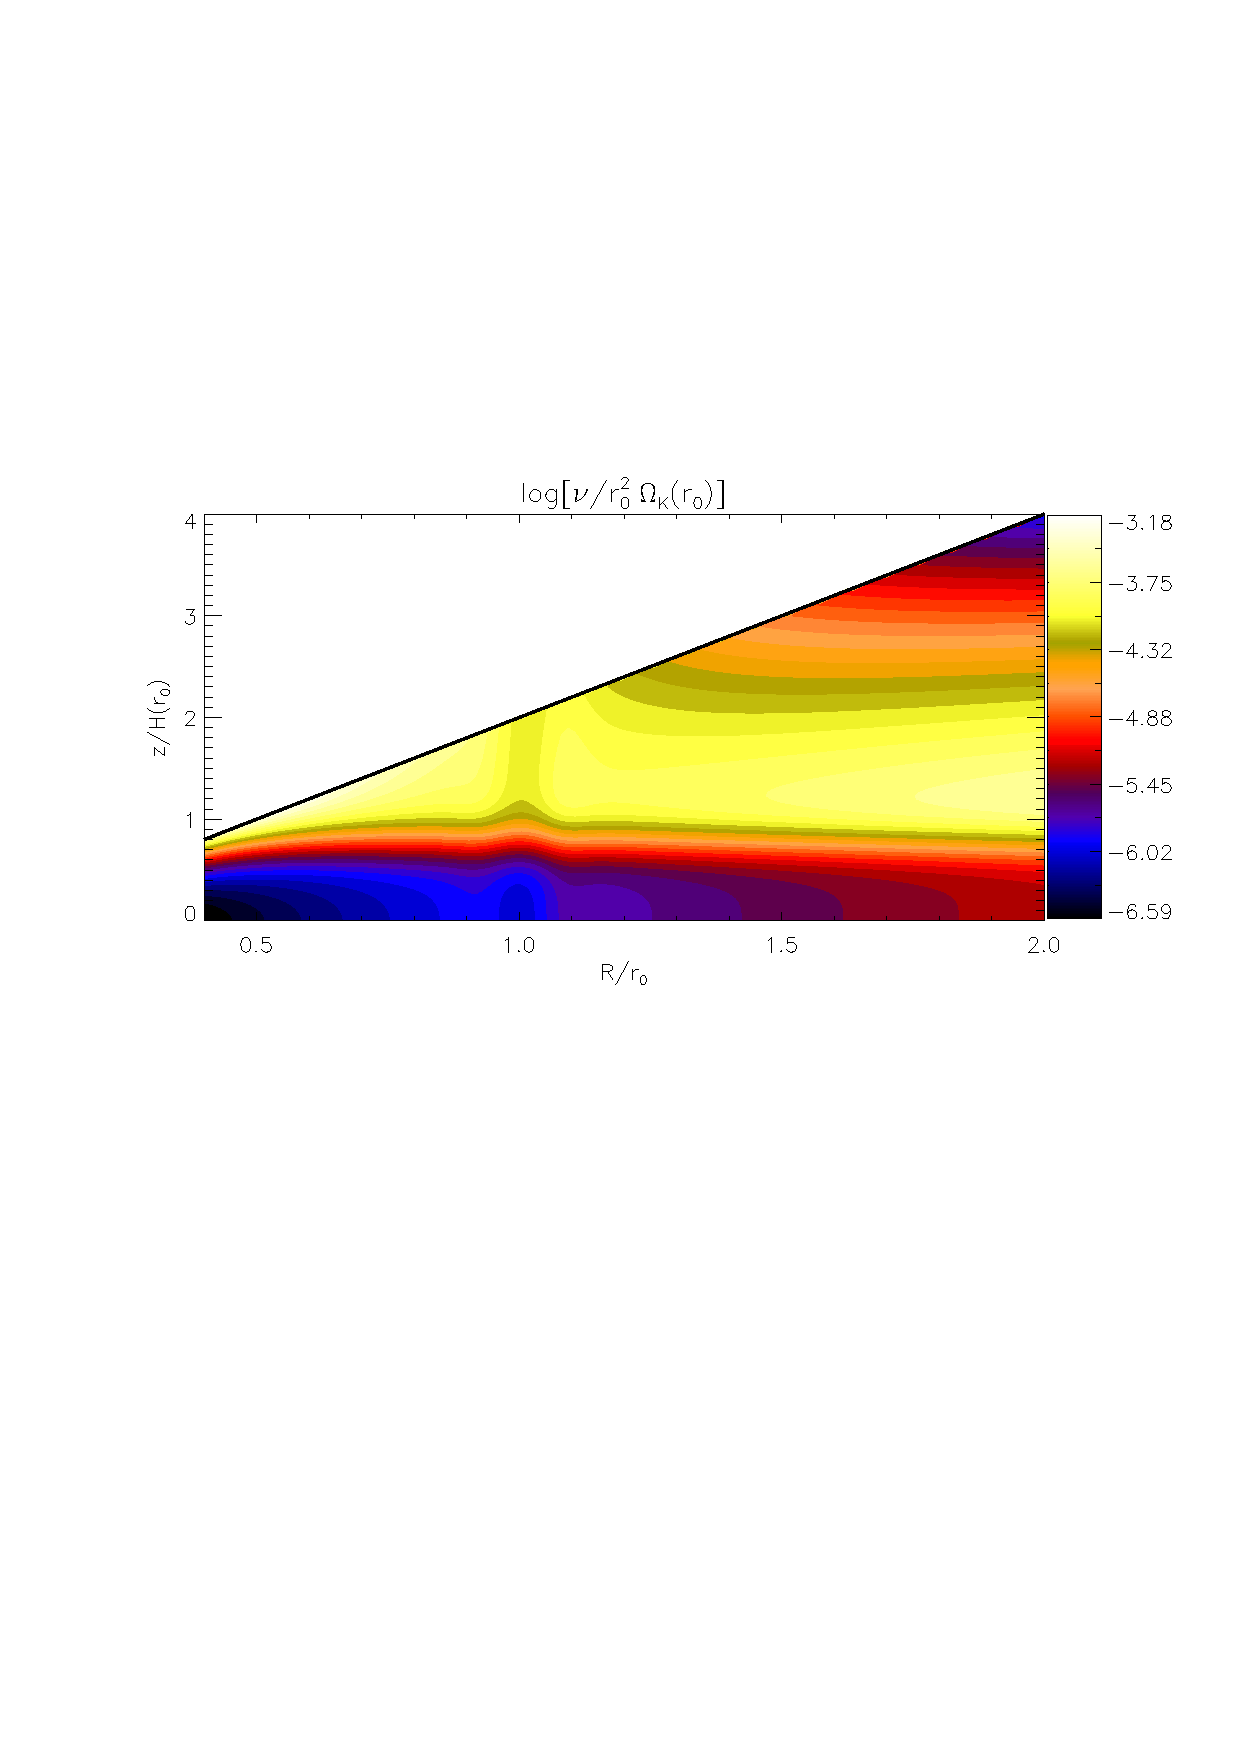
\includegraphics[width=\linewidth]{figures/pdisk_visc2d_layer2}
  \caption{Example of a two-layered kinematic viscosity profile
    resulting from Eq. \ref{visc_profile}. This specific plot
    corresponds to case V2. The solid line
    delineates the upper boundary of the computational domain.
    \label{visc2d}}
\end{figure}


\subsection{Simulations}
We consider discs with radial extent $[\rin,\rout]=[0.4,2.0]r_0$,
vertical extent $n_h=2$ scale-heights and aspect-ratio $h=0.1$ at
$R=r_0$. We use $(N_r, N_\theta,
N_\phi)=(256,64,512)$ grid points. 
The resolution at the reference radius is then
$16,\,32,\,8$ cells per scale-height in $(r,\theta,\phi)$ directions,
respectively. The planet potential is disabled for these runs
($M_p\equiv 0$). We apply a damping rate $\hat{\gamma}=1$ with the
reference velocity $\bm{v}_\mathrm{ref}=\bm{v}(t=0)$.     

The bump parameters are set to $A=1.25$ and $\Delta R = 0.05r_0$ for
all runs in this section. The spherical radial velocity is subject 
to random perturbations of magnitude $10^{-4}c_s$ 
a few time-steps after initialisation. 

\subsubsection{Inviscid run}
For reference we simulate an effectively inviscid disc, case B0,
with the viscosity parameters $\hat{\nu}_0=10^{-9}$ and $A_\nu = 1$.  
Thus viscosity is independent of $z$ at $R=r_0$.   
Inviscid setups similar to case B0 have previously been simulated
both in the linear and non-linear regimes  \citep{meheut12, lin13}. 
%So, %in addition to a control run, case B0 also serves to test the \pluto
%code in simulating the RWI.    

\subsubsection{Viscous runs}
In these runs the floor viscosity is 
$\hat{\nu}_0=10^{-6}$. The control run case V0 has $A_\nu =
1$. Thus, case V0 is the viscous version of case B0.  
We then consider models where the kinematic viscosity increases by
a factor $A_\nu=100$ for $z>\zeta_\nu H_0$ at the bump radius. We
choose $\zeta_\nu=1.5,\,1.0$ for cases V1 and V2, respecively.  This
gives a upper 
viscous layer of thickness $0.5H$ and $H$ at $R=r_0$. (See
Fig. \ref{visc2d} for a plot of the kinematic viscosity profile for case V2.) 
For case V1 and V2 the transition thickness is fixed to
$\Delta\zeta_\nu=0.2$.  
 
Finally, we consider a high viscosity run, case V3, 
with $\hat{\nu}_0=10^{-4}$ and $A_\nu=1$.  This is equivalent to
extending the viscous layer in case V1/V2 to the entire vertical
domain.  

\subsubsection{Linear growth rates and frequencies}
The present setup allows us to define a linear instability in the
usual way: exponential growth of perturbations measured with respect
to an axisymmetric steady equilibrium. A proper linear
stability analysis, including the full viscous stress tensor, is
beyond the scope of this paper, but we can nevertheless extract linear 
mode frequences from the non-linear simulations.  

The $m^\mathrm{th}$ Fourier component of the density field is  
\begin{align}
\hat{\rho}_m(r,\theta,t) \equiv \int_0^{2\pi} \rho(\bm{r},t)\exp{(-\ii
  m\phi)}d\phi. 
\end{align} 
The magnitude of a Fourier mode is measured by 
\begin{align} 
a_m(t)\equiv \frac{b_m(t)}{b_0(0)},\quad b_m(t)\equiv \avg{|\hat{\rho}_m|}_r,
\end{align} 
where $\avg{\cdot}_r$ denotes averaging over a spherical shell (to be
chosen later). 
The complex frequency $\sigma_m$ associated with the $m^\mathrm{th}$ component 
is defined through 
\begin{align}\label{sigma}
  \frac{\p\hat{\rho}_m}{\p t} \equiv -\ii\sigma_m\hat{\rho}_m. 
\end{align}
The time derivative in Eq. \ref{sigma} can be computed implicitly by 
Fourier-transforming the continuity equation \citep[as done
  in][]{lin13}. 

In a linear stability problem $\sigma_m$ is a constant eigenvalue. 
However, when extracted numerically from a non-linear simulation, 
we will generally obtain $\sigma_m=\sigma_m(r,\theta,t)$. Thus, we compute 
$\avg{\sigma_m}_r = m\omega_m + \ii q_m$    
where $\omega_m$ is the mode frequency and $q_m$ is the growth rate.
We normalise the linear frequencies by
$\Omega_0\equiv\Omega_i(r_0)\simeq\Omega_k(r_0)$. 

\subsection{Results}
Table \ref{artificial_bump} summarises the simulations presented in
this section. Linear mode frequencies are measured at 
$t=10P_0$ (when $|\delta\rho|\ll 1$) and averaged over 
$r\in[0.8,1.2]r_0$. The second set of measurements is made well into
the non-linear regime at $t=100P_0$. 
The minimum Rossby number is measured at
the midplane.  

\begin{table*}
  \centering
  \caption{Summary of hydrodynamic simulations initialized with a
    density bump. 
    $\hat{\nu}_0=10^{-4}$ and $A_\nu=1$. \label{artificial_bump}}
  \begin{tabular}{lcccccl @{\extracolsep{0.1cm}} ccc}
    \hline\hline
    \multicolumn{4}{c}{\phantom{stuff}} &
    \multicolumn{3}{c}{$t = 10P_0$ (linear phase)}&
    \multicolumn{3}{c}{$t=100P_0$}\\
    \cline{5-7}\cline{8-10}
    Case  & $\log{\hat{\nu}_0}$ & $A_\nu$ &$\zeta_\nu$ & $m$ &
    $\omega_m/\Omega_0$ &
    $q_m/\Omega_0$ &  
    $m$ & $10^2a_m$ & $\mathrm{min}[Ro(z=0)]$ \\ 
    \hline
    B0 &-9 & 1 &n/a & 4 & 0.985  & 0.199  %omit = 3
    &  1 & 8.5  & -0.15   \\  
    
    V0  &-6 & 1 &n/a &  4 & 0.985  & 0.199   
    & 1 & 6.8 &  -0.11  \\
    
    V1  &-6 & 100 & 1.5  & 4 & 0.986  & 0.191
    &  1 & 7.8 &  -0.19 \\
    
    V2  & -6 & 100 & 1.0  &  4  & 0.986  & 0.182  
    &  1 & 4.9 &  -0.21 \\
    
    V3  & -4 & 1 & n/a  &  4  & 0.986  &  0.131  
    &  3 &  3.7  &  -0.25 \\
   \hline
  \end{tabular}
\end{table*}

\subsubsection{Inviscid reference case}
Fig. \ref{bump0_bump1} 
shows the density fluctuation and Rossby number for
case B0. The dominant linear mode is $m=4$ with a growth rate
$0.2\Omega_0$, consistent with recent 3D linear calculations 
\citep{meheut12,lin13}. 
%Fig. \ref{bump0_bump1} shows that the
%linear phase consists of non-axisymmetric vorticity perturbations on
%either side of the density bump \citep{umurhan10}, i.e. vorticity
%waves propagating along the PV gradients.     
The non-linear outcome of the RWI is vortex formation
\citep{li00}. Four vortices develop initially, then 
merge on a dynamical timescale into  
a single vortex. Case B0 evolves similarly to previous simulations of
the RWI in an inviscid disc 
\citep[e.g.][where more detailed analyses are 
given]{meheut10,meheut12b}. This, together with the agreement with
linear calculations, demonstrates the ability of the \pluto
code to capture the RWI. 

\begin{figure}
  \centering
  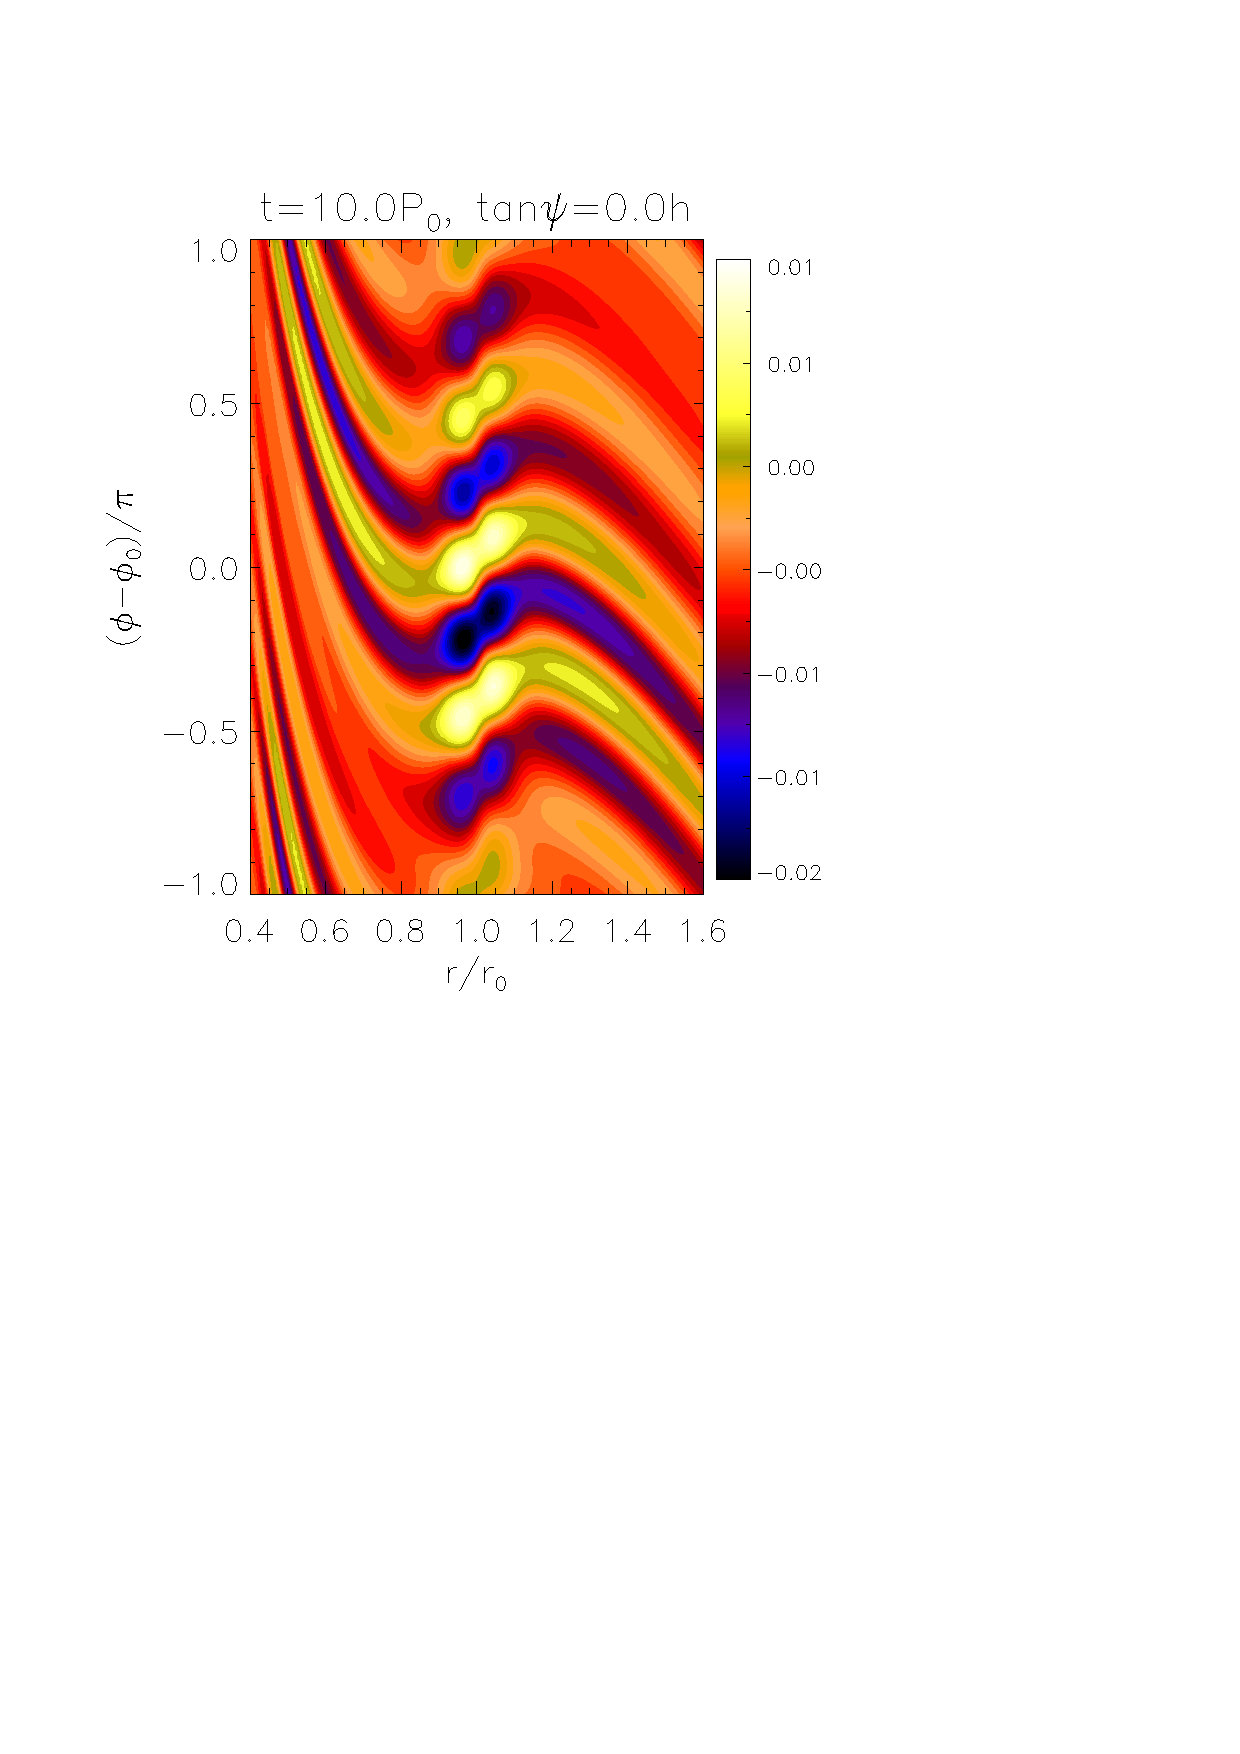
\includegraphics[scale=.27,clip=true,trim=0cm 0.9cm 0cm
    0cm]{figures/bump0_pdisk001}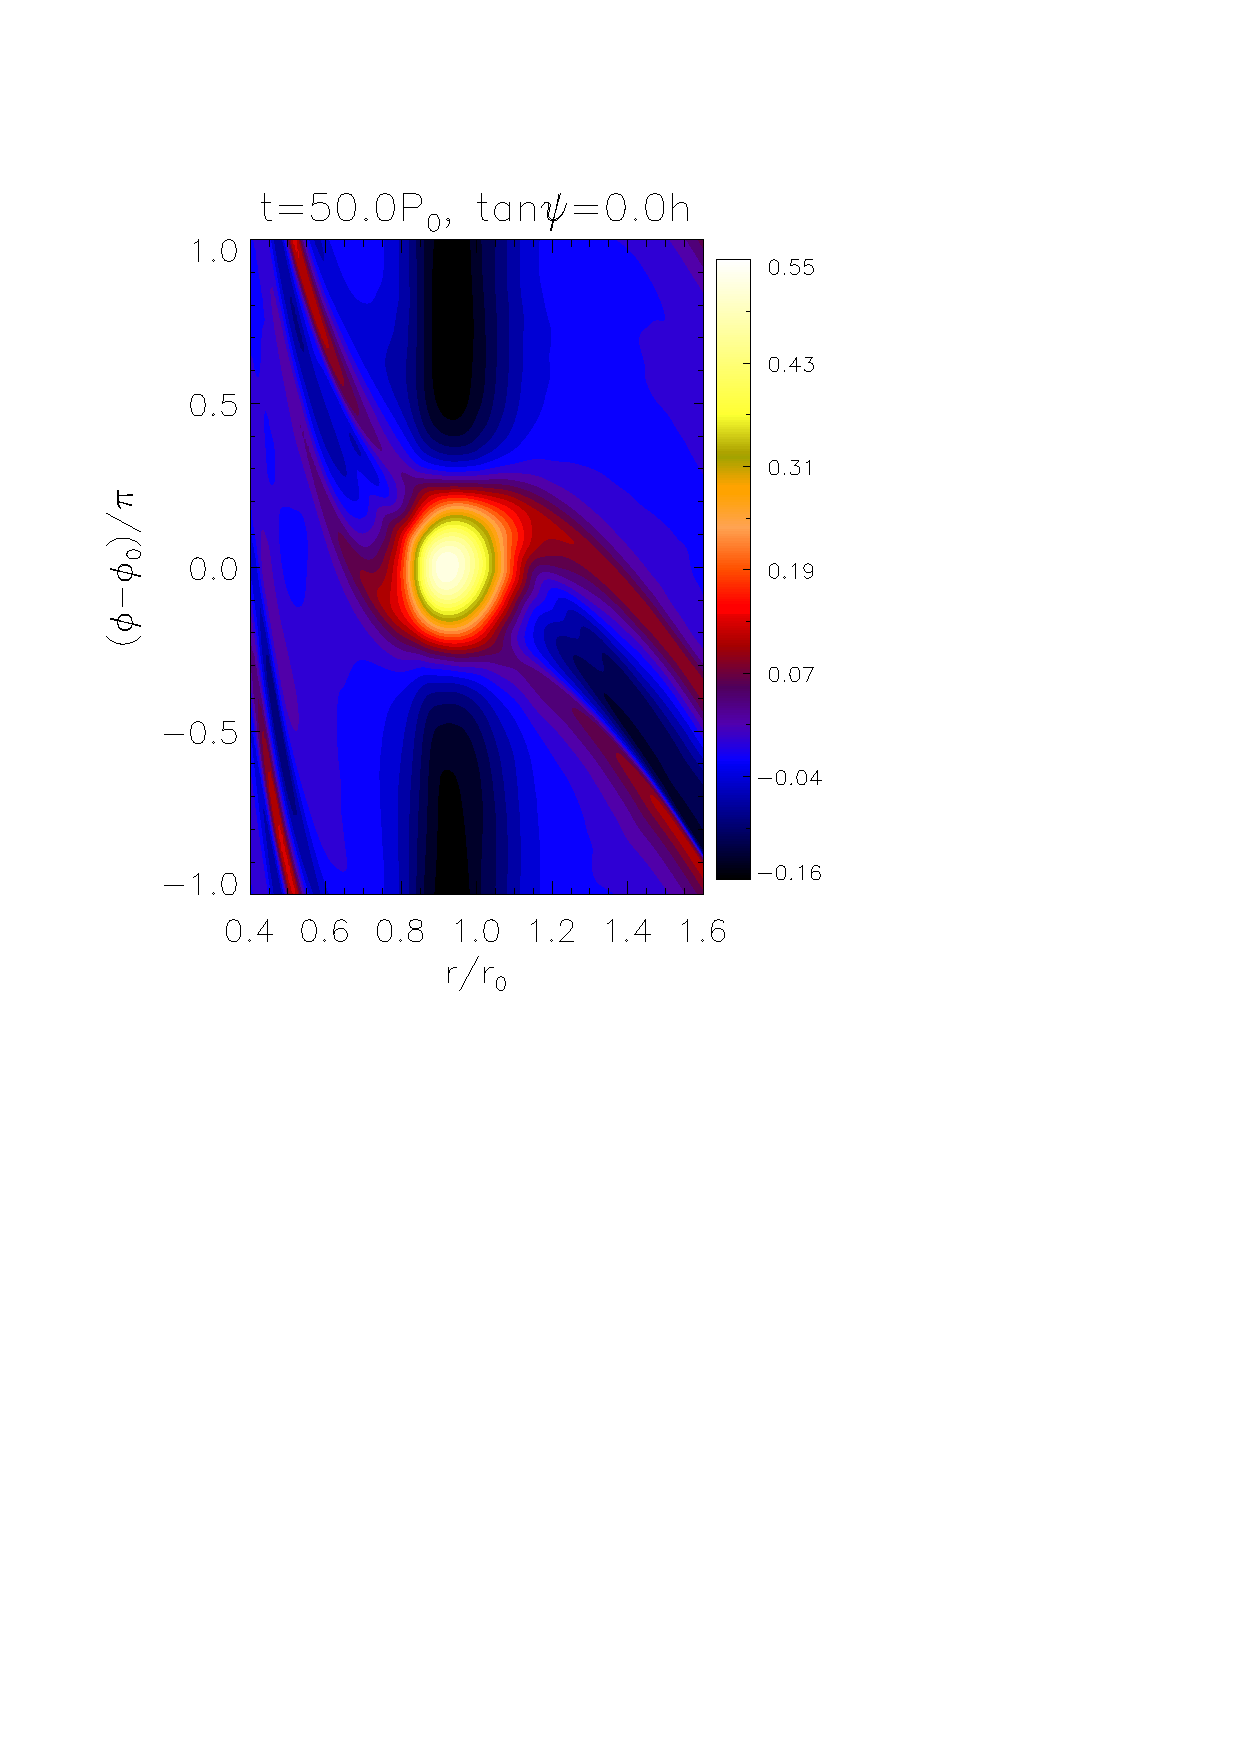
\includegraphics[scale=.27,clip=true,trim=2.3cm
    0.9cm 0cm
    0cm]{figures/bump0_pdisk005}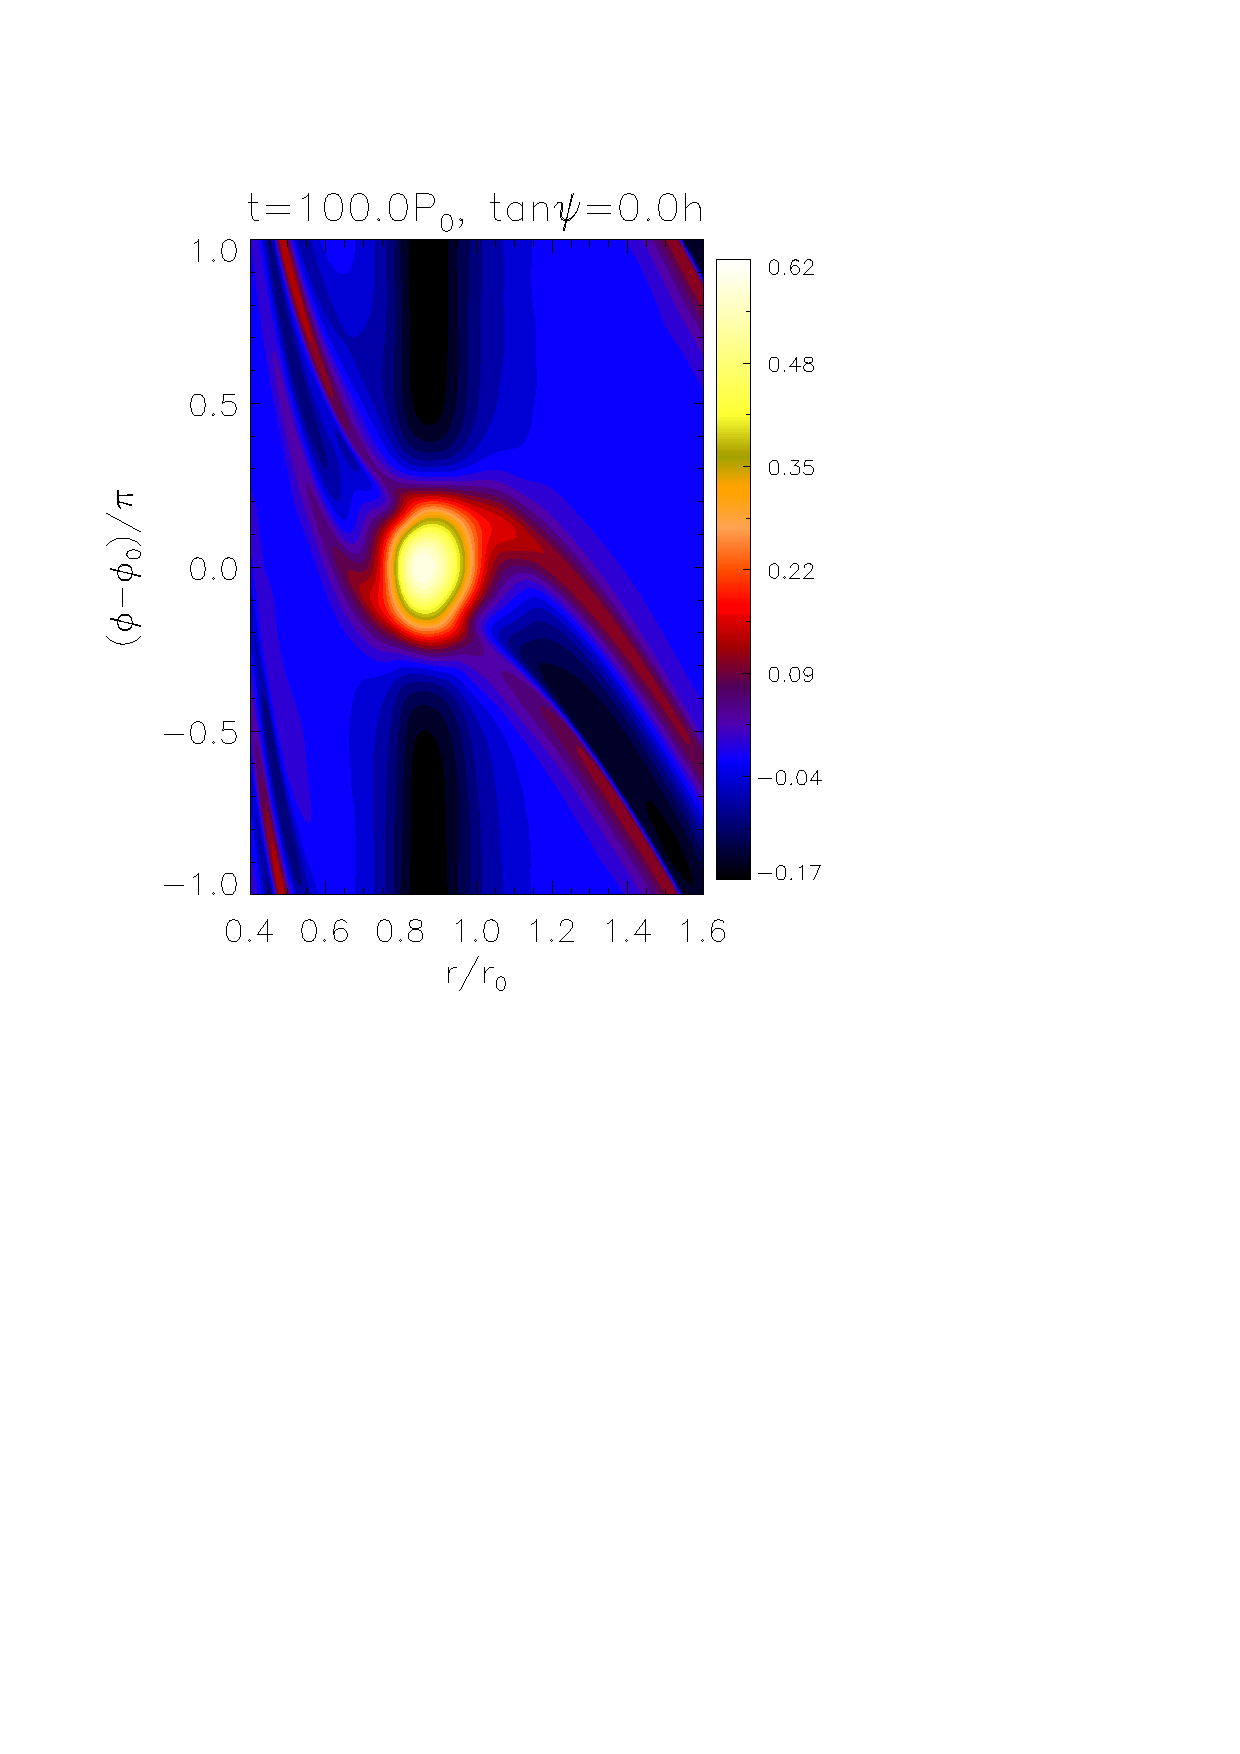
\includegraphics[scale=.27,clip=true,clip=true,trim=2.3cm
    0.9cm 0cm
    0cm]{figures/bump0_pdisk010}
   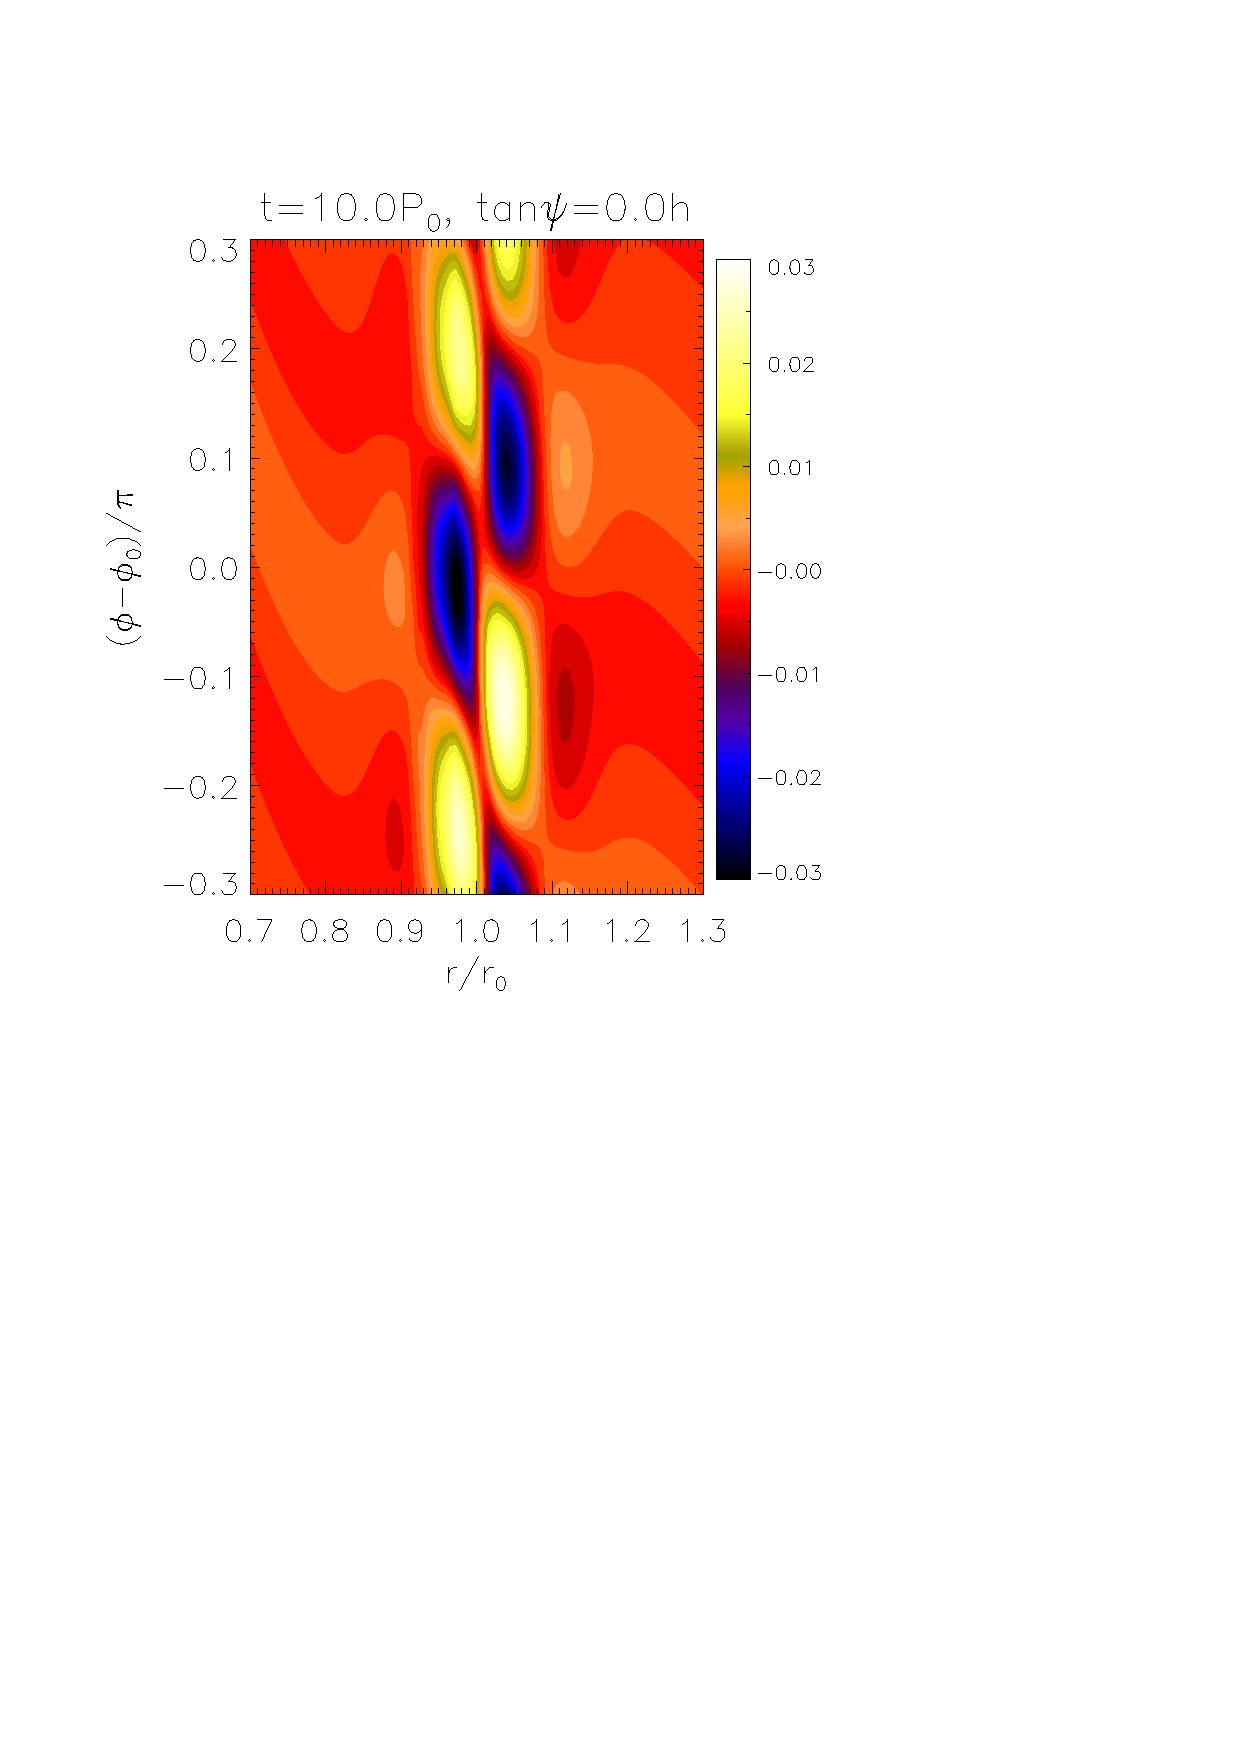
\includegraphics[scale=.27,clip=true,trim=0cm 0.cm 0cm
     0.9cm]{figures/bump0_vort001}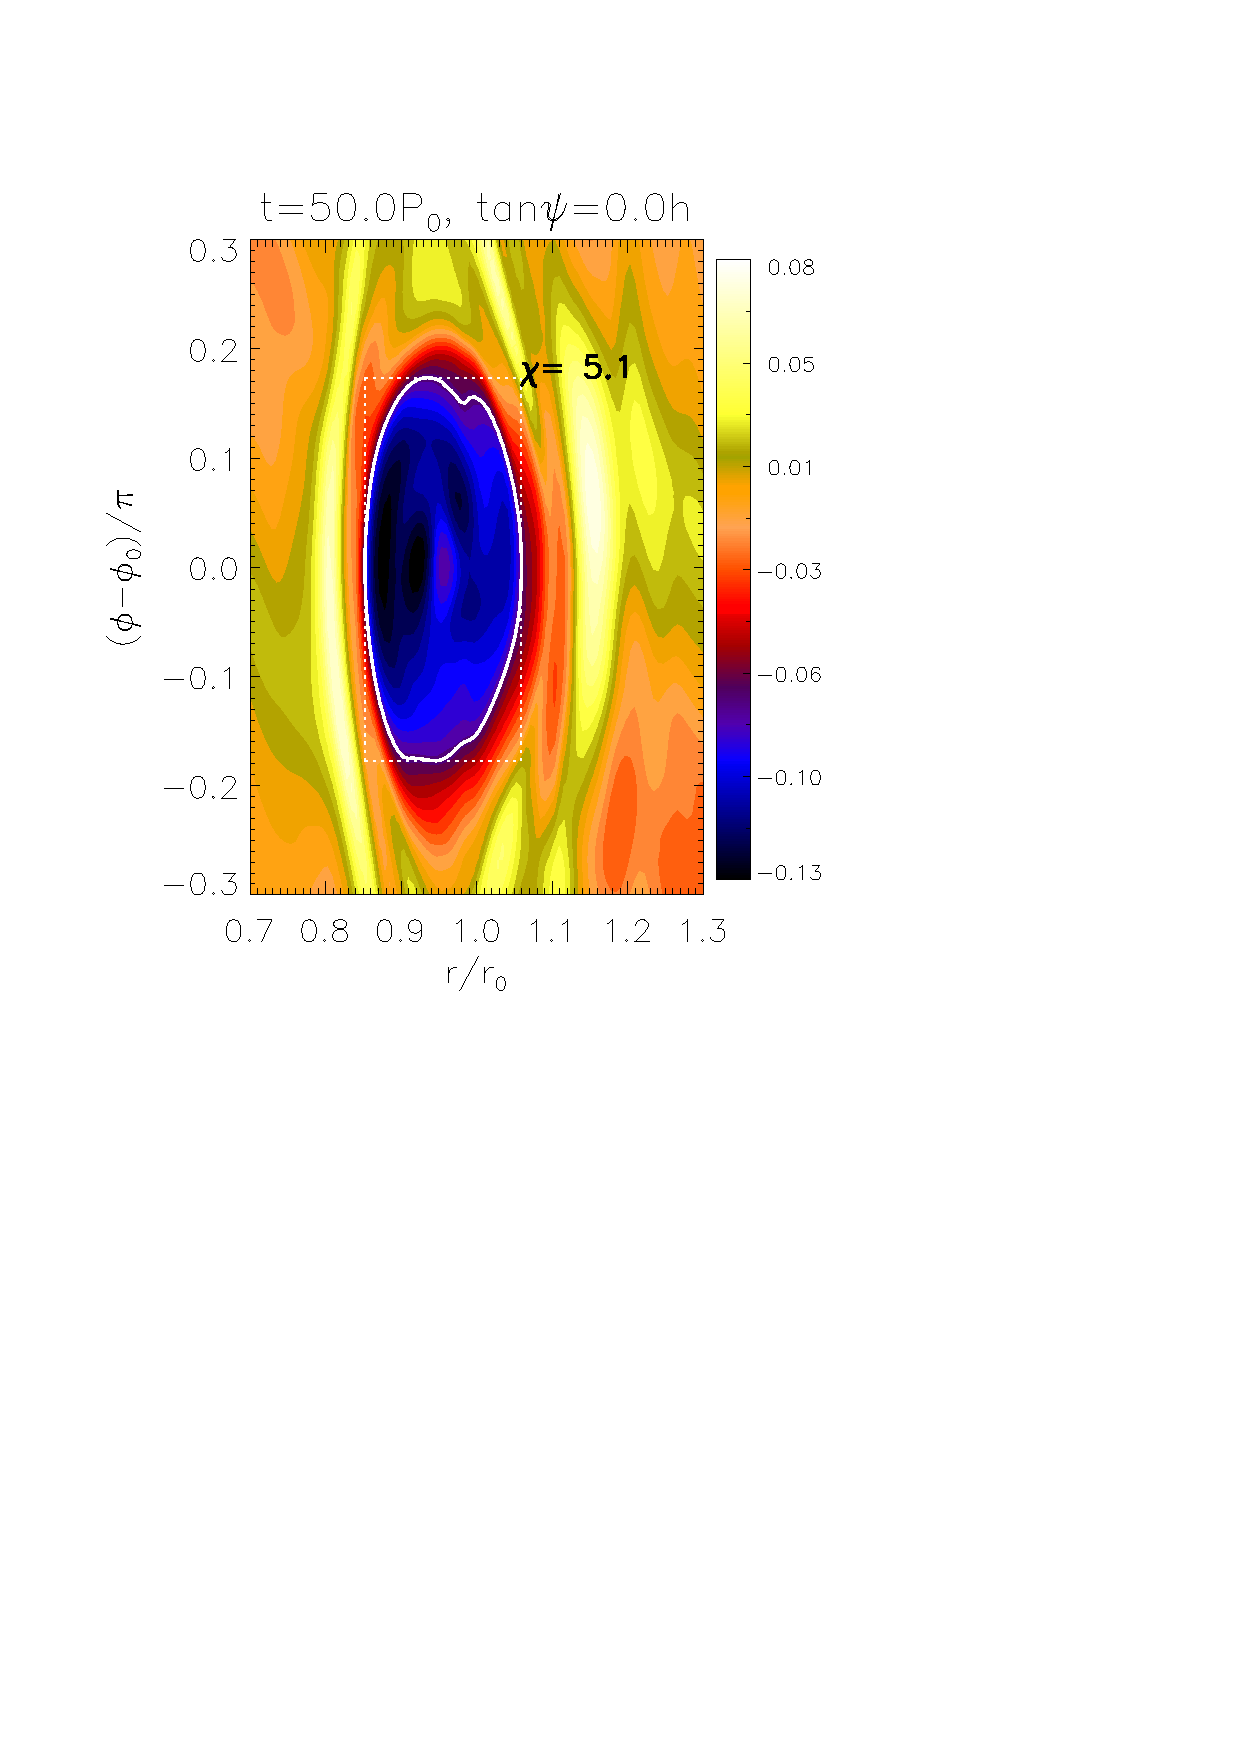
\includegraphics[scale=.27,clip=true,trim=2.3cm
     0.cm 0cm
     0.9cm]{figures/bump0_vort005}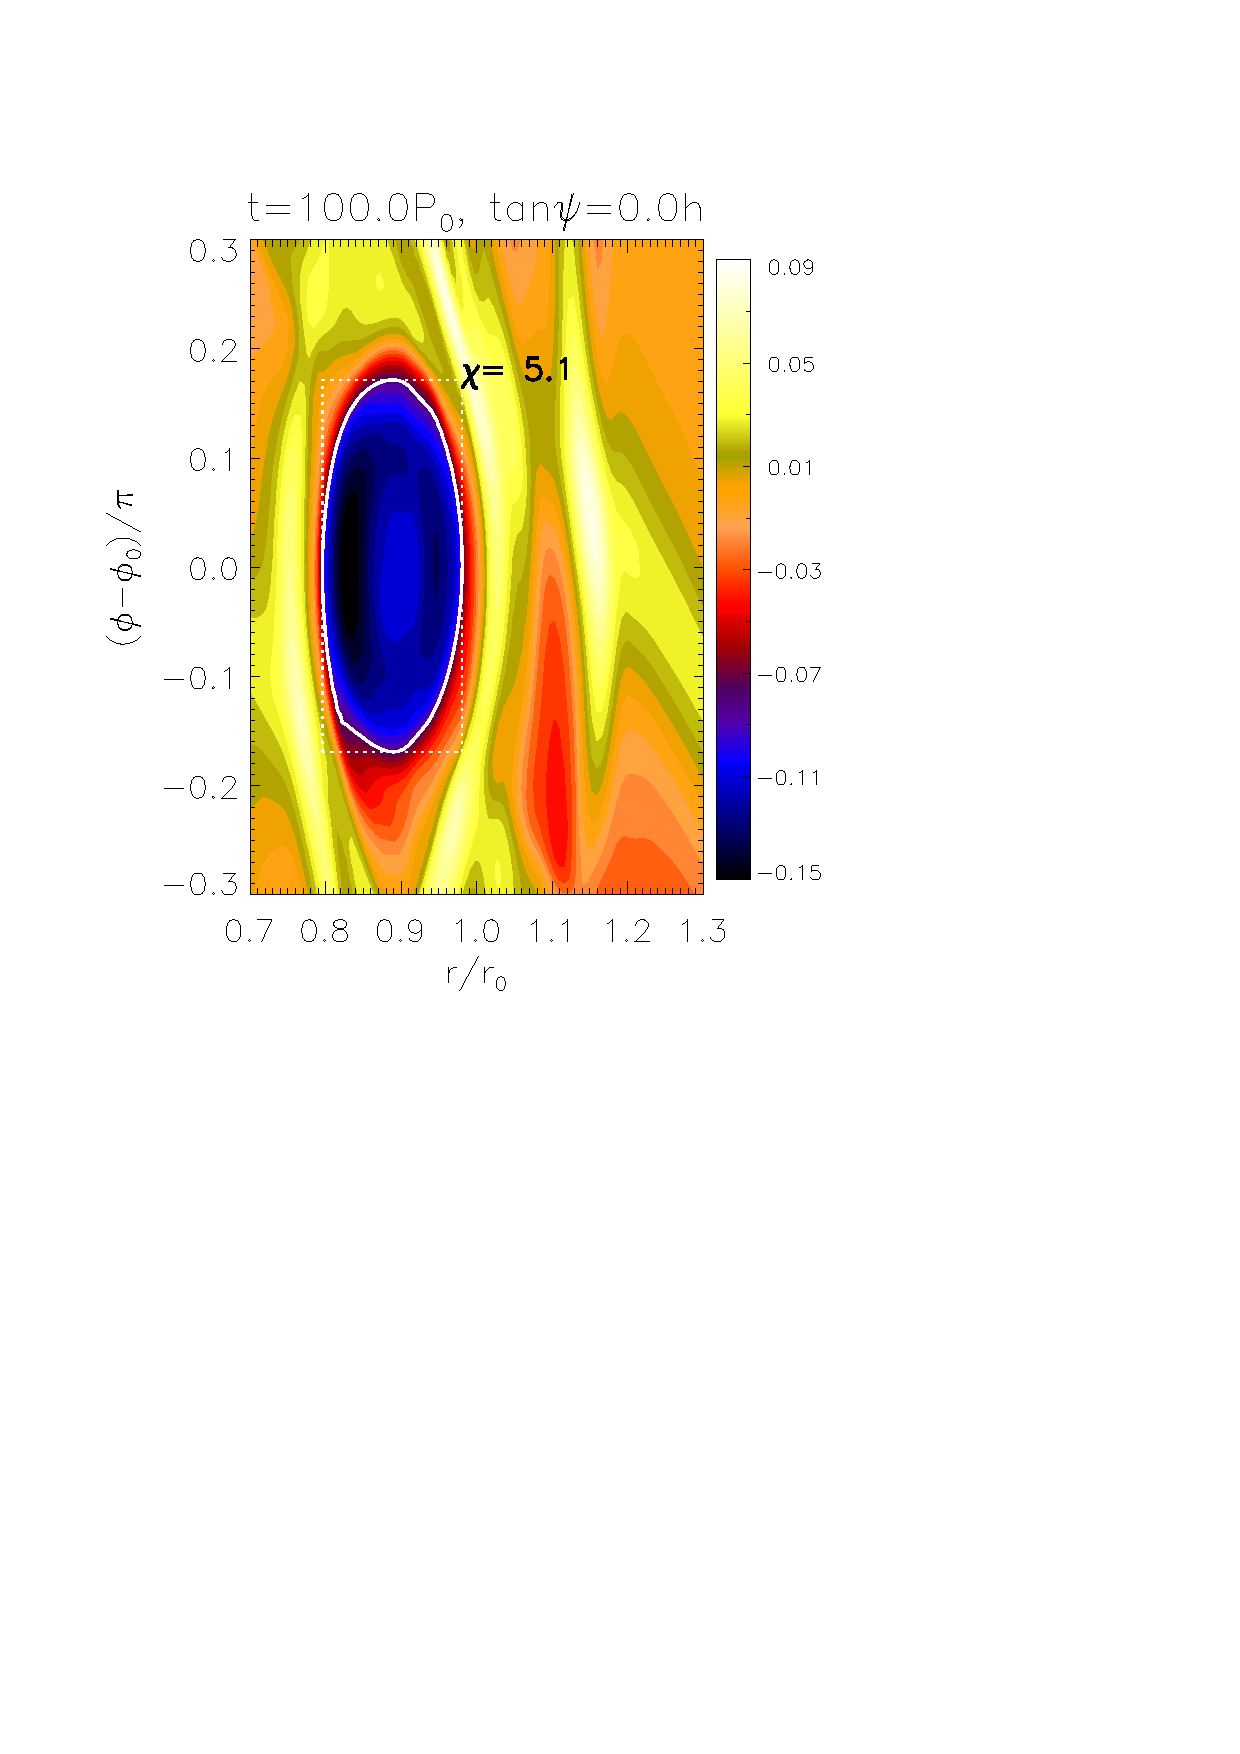
\includegraphics[scale=.27,clip=true,clip=true,trim=2.3cm
     0.cm 0cm
     0.9cm]{figures/bump0_vort010}
  \caption{Evolution of the inviscid case B0. Top: midplane density fluctuation, 
    $\Delta\rho(z=0)$. Bottom: midplane
    Rossby number (note the different axis range from the top panel). 
    Here, $\chi$ is an empirical measure of the final vortex
    aspect-ratio. $\phi_0$ is the azimuth of 
    $\mathrm{max}\left[|\Delta\rho(z=0)|\right]$.
    \label{bump0_bump1}}
\end{figure}

\subsubsection{The effect of a viscous layer}
We now examine viscous cases V0 --- V3. Recall  
from Table \ref{artificial_bump} that the viscous layer (with $
\hat{\nu}\sim10^{-4}$) occupies the uppermost $0\%,\,25\%,\,50\%$ and
$100\%$ of the vertical domain at $R=r_0$ for cases V0, V1, V2 and V3,
respectively.     

We first compare the viscous case V0 to the 
inviscid case B0. Table \ref{artificial_bump} shows that despite
increasing the viscosity by a factor of $10^3$, the change to the
linear mode frequencies are negligible. 
The value of $a_m$ and minimum Rossby number indicate that the final
vortex in V0 is only slightly weaker than that in B0. This is also
reflected in  Fig. \ref{bump0_bump1} (case B0) and the leftmost column in
Fig. \ref{vdamp0} (case V0). Case V0 develops a more elongated 
vortex with smaller $|\Delta\rho|$ than that in B0. 
  
As we introduce and thicken the viscous layer from case V0 to V3, the dominant
linear mode remains at $m=4$ (Table \ref{artificial_bump}), but linear
growth rate does appreciably decrease (by $\sim 34\%$ from case V0 to
V3). However, these linear growth timescales  
are still $\sim P_0$. We thus have the important result that
viscosity (layered or not) does not significantly affect the linear
instability because the RWI grows dynamically even in the high
viscosity disc.     
 
\begin{figure*}
   \centering
   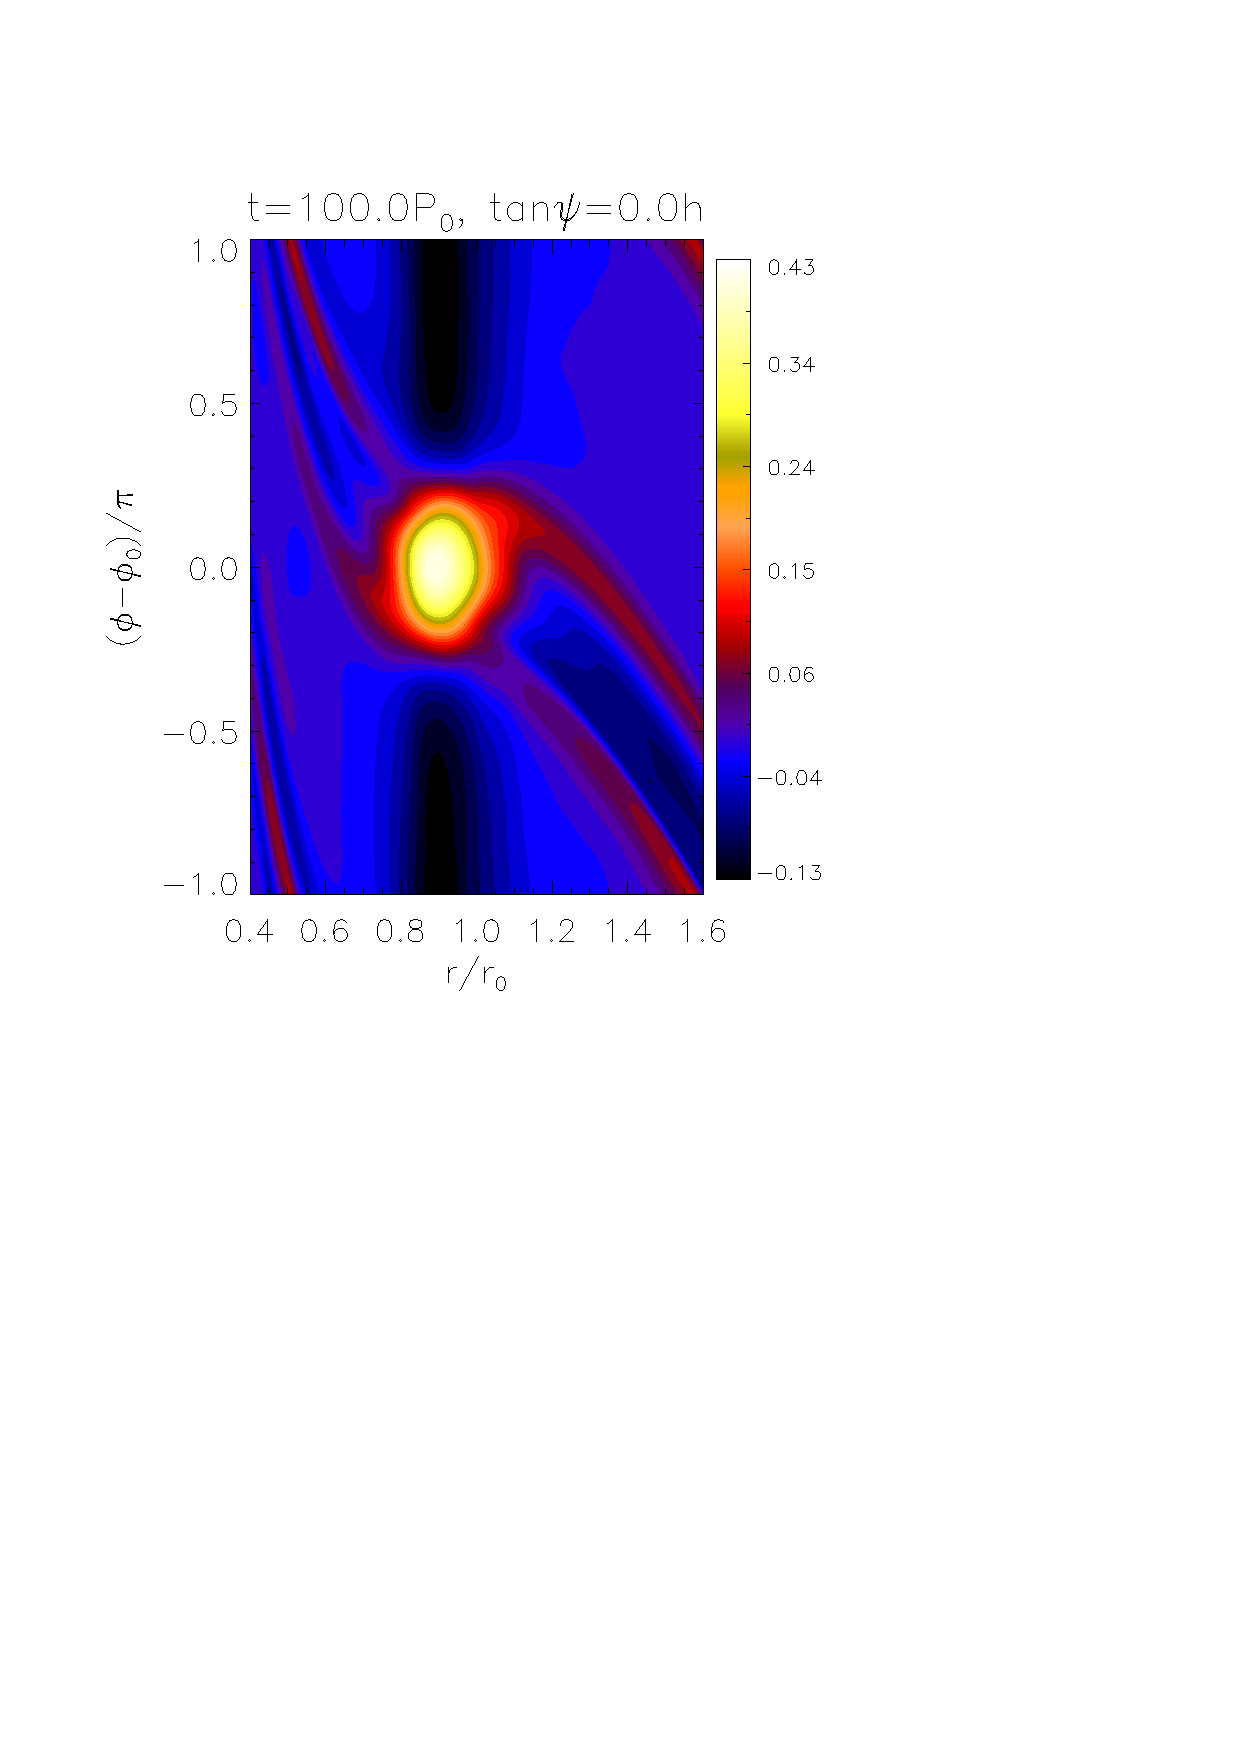
\includegraphics[scale=.43,clip=true,trim=0cm 0.9cm 0cm
     0.99cm]{figures/vdamp0_pdisk010}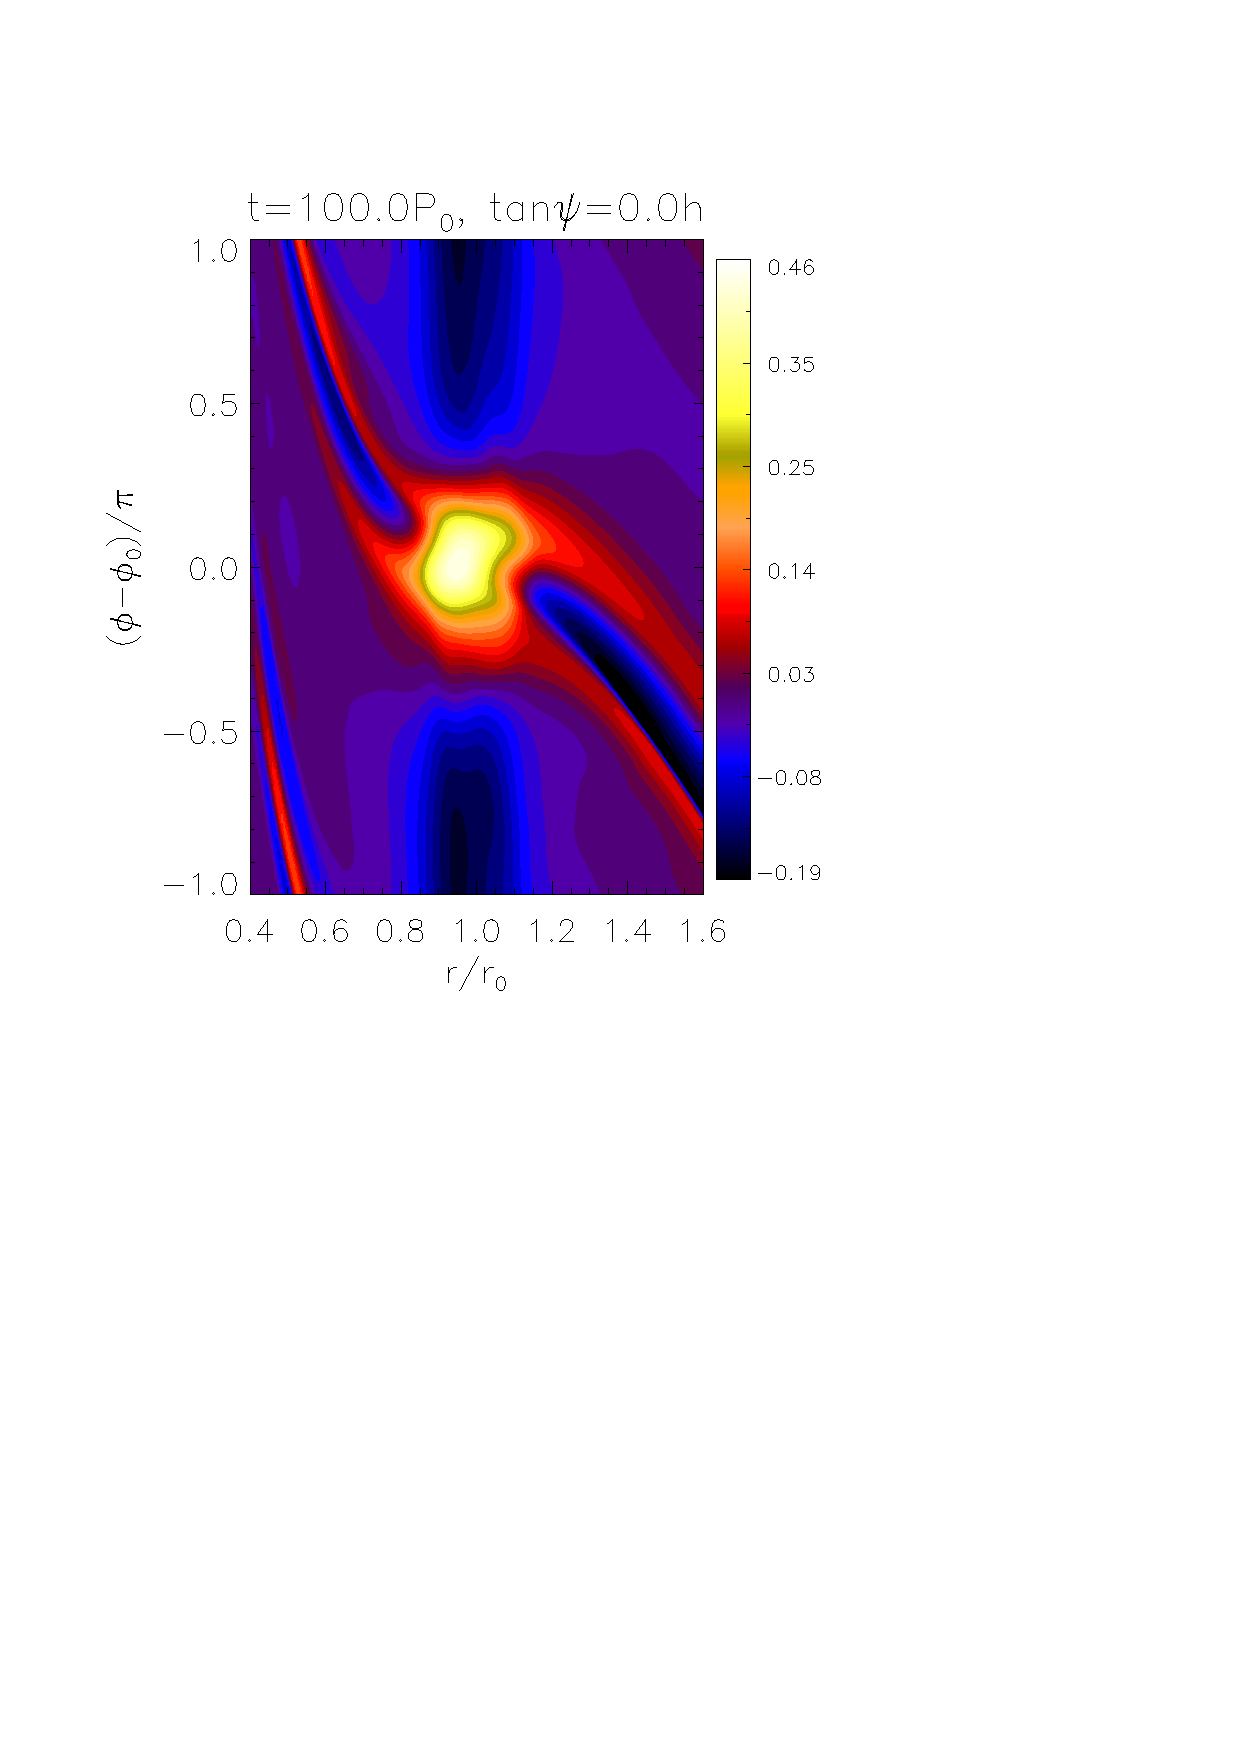
\includegraphics[scale=.43,clip=true,trim=2.3cm
     0.9cm 0cm
     0.99cm]{figures/vdamp2_pdisk010}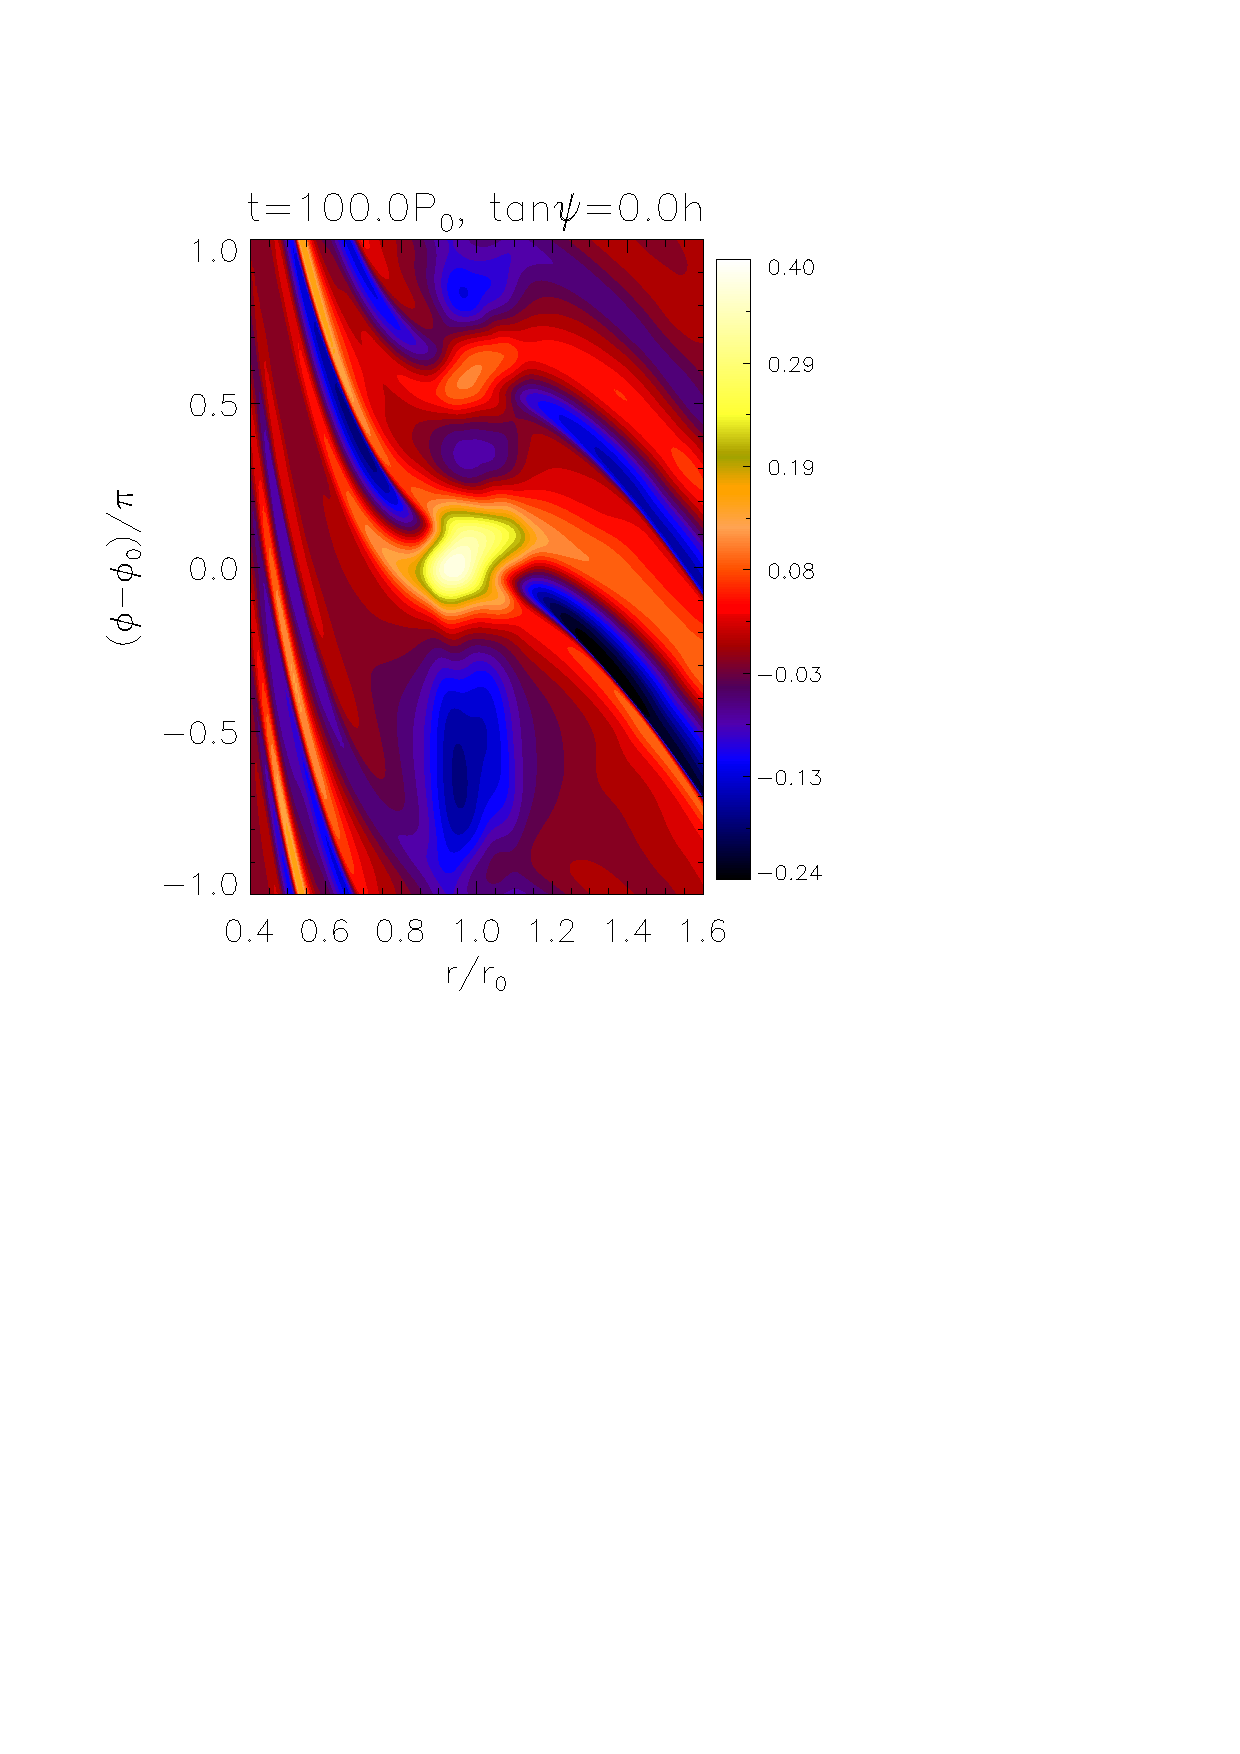
\includegraphics[scale=.43,clip=true,trim=2.3cm 
     0.9cm 0cm
     0.99cm]{figures/vdamp3_pdisk010}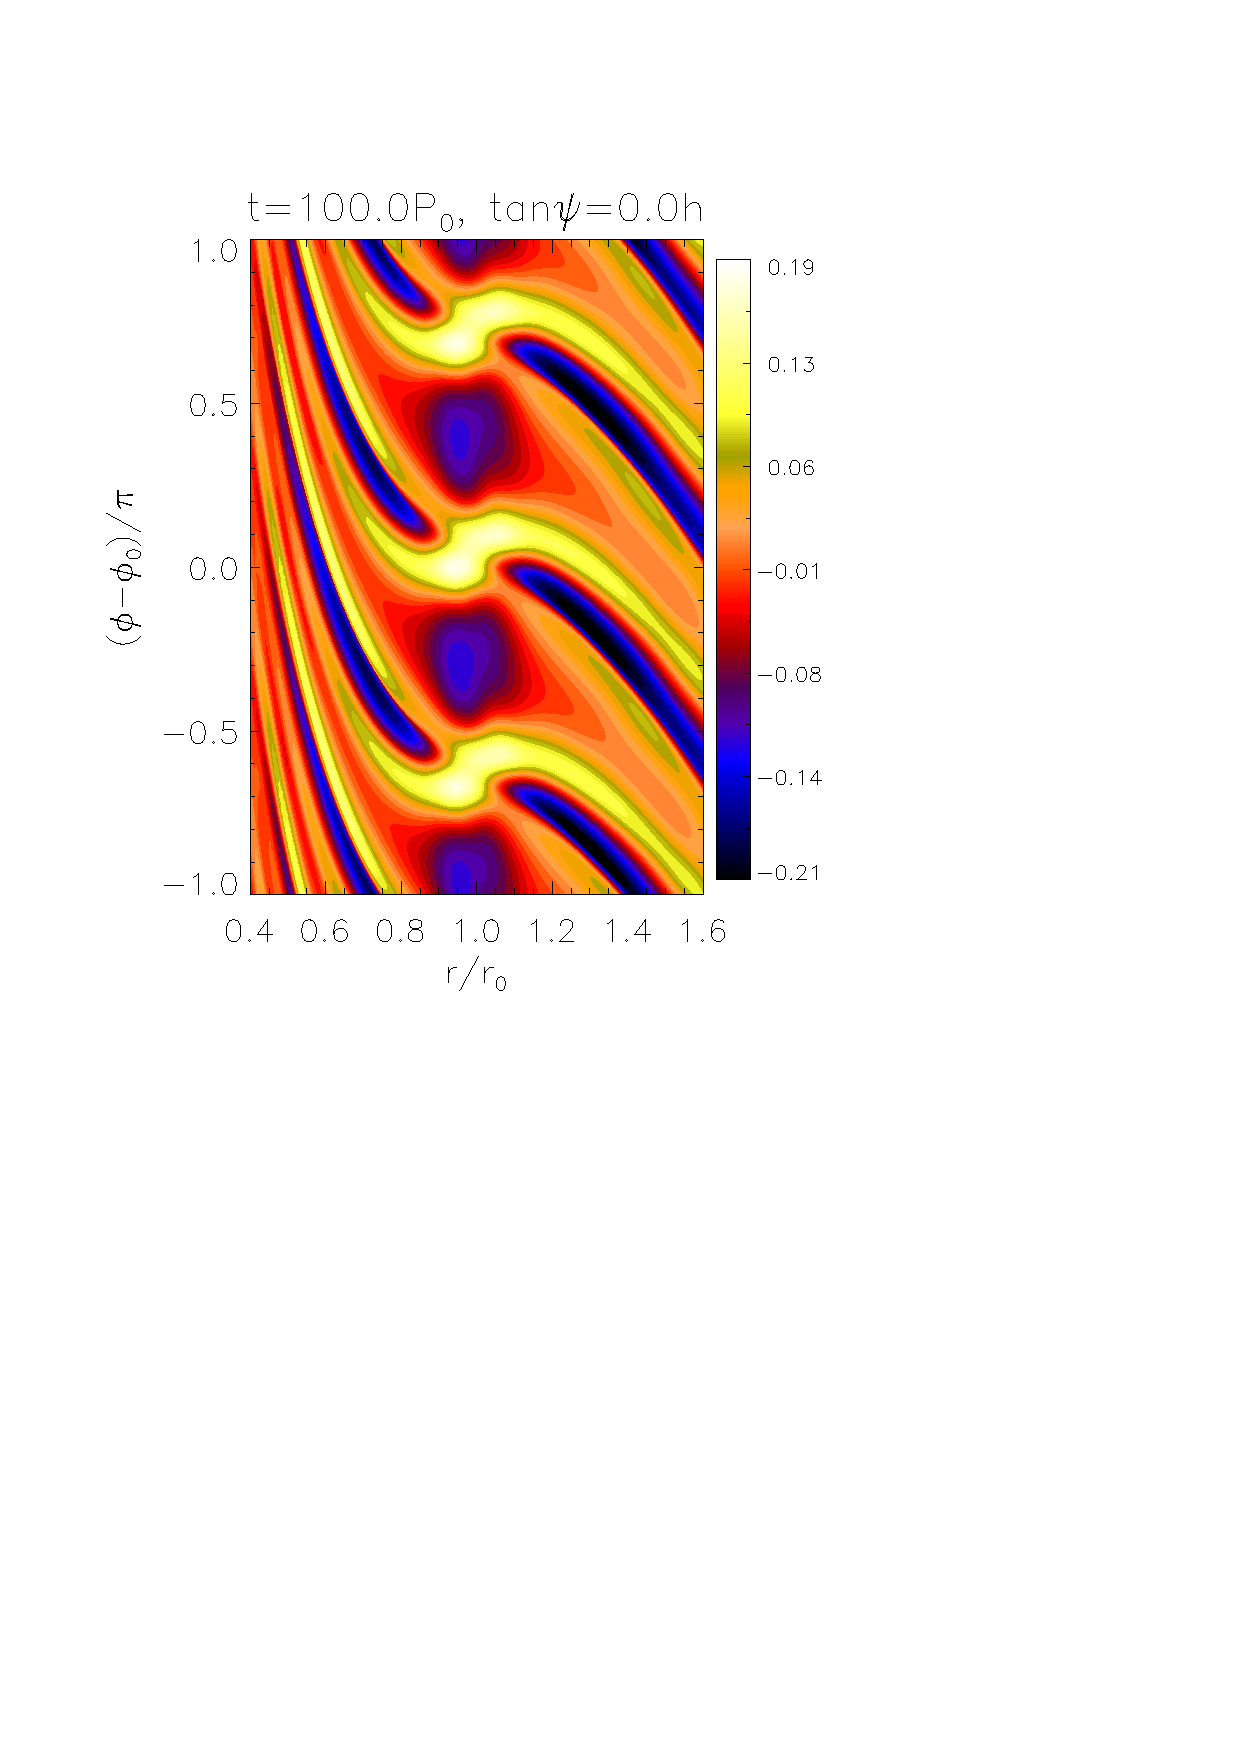
\includegraphics[scale=.43,clip=true,trim=2.3cm
     0.9cm 0cm
     0.99cm]{figures/vdamp0_nu4_pdisk010}\\
      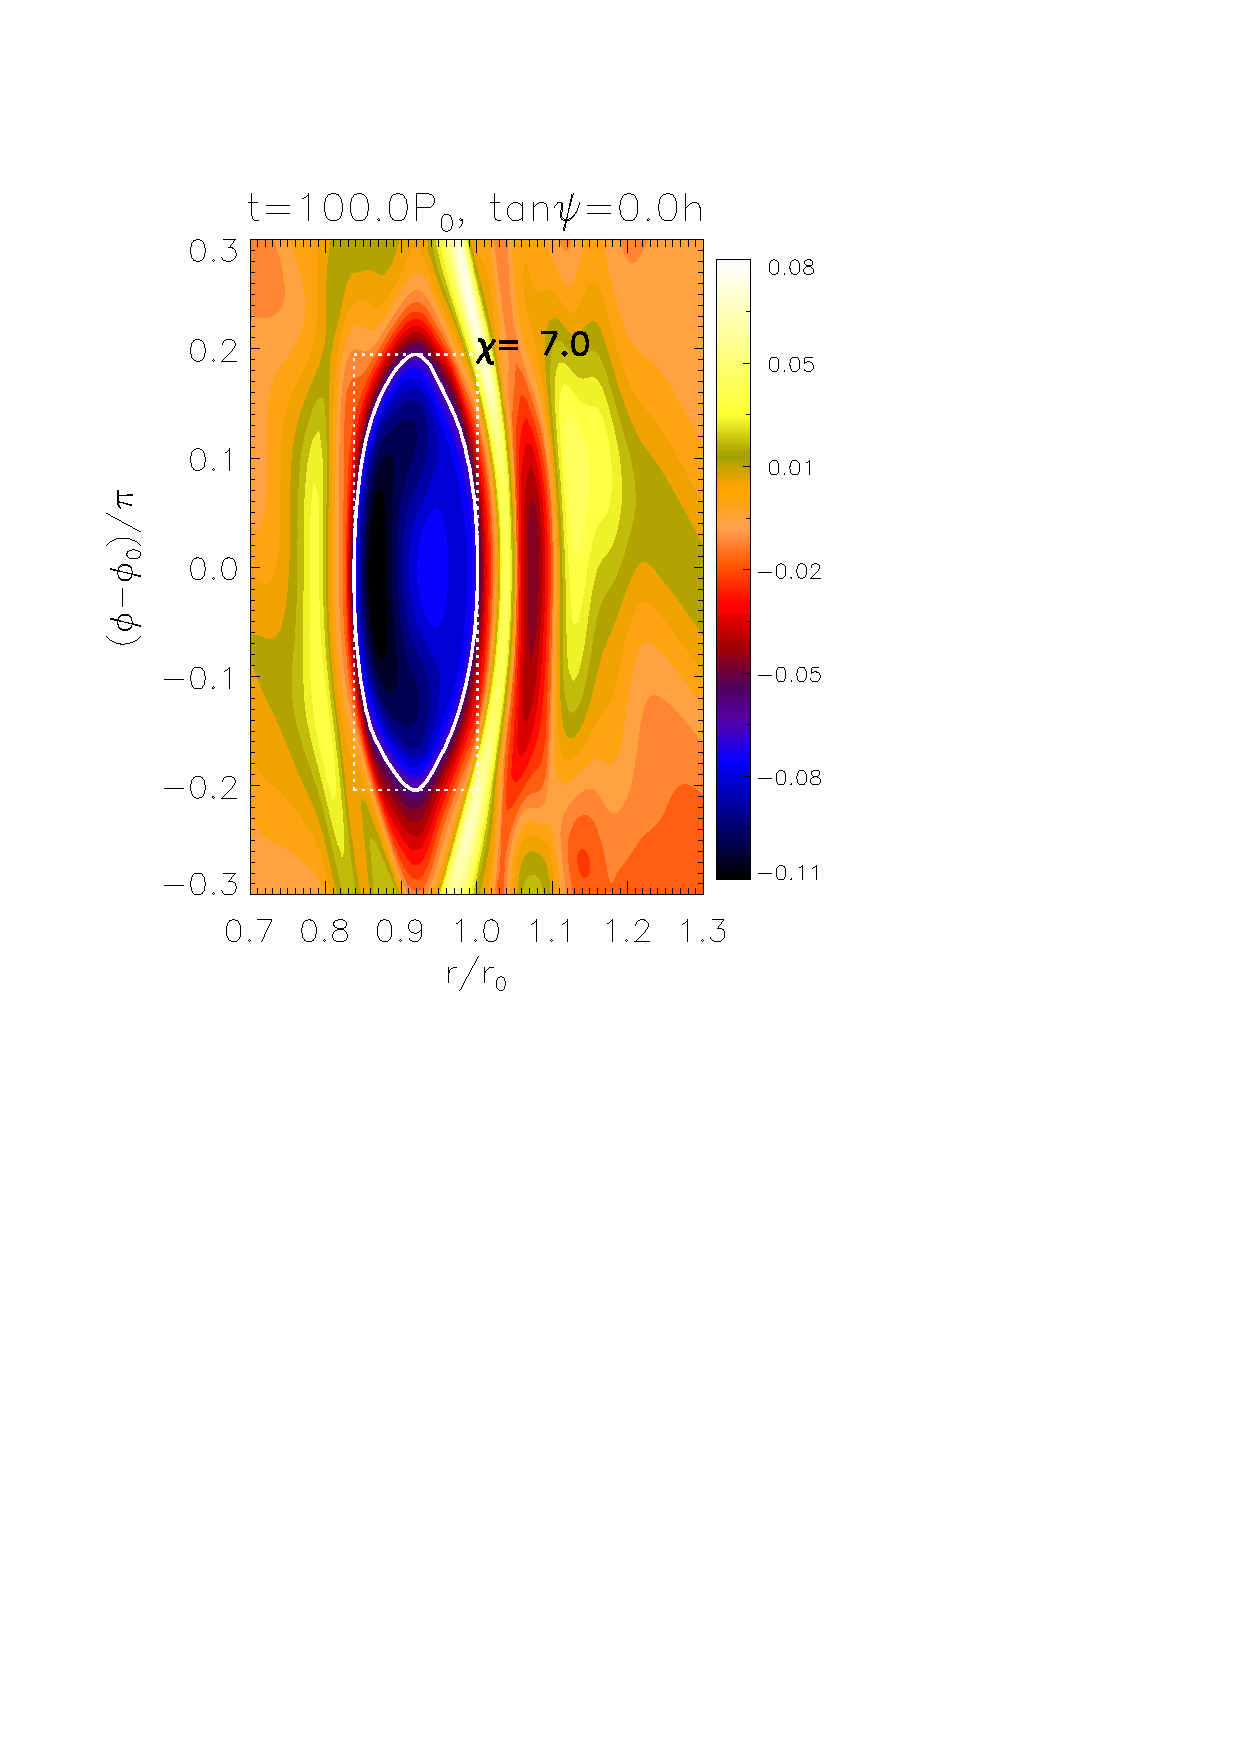
\includegraphics[scale=.43,clip=true,trim=0cm 0.cm 0cm
     0.99cm]{figures/vdamp0_vort010}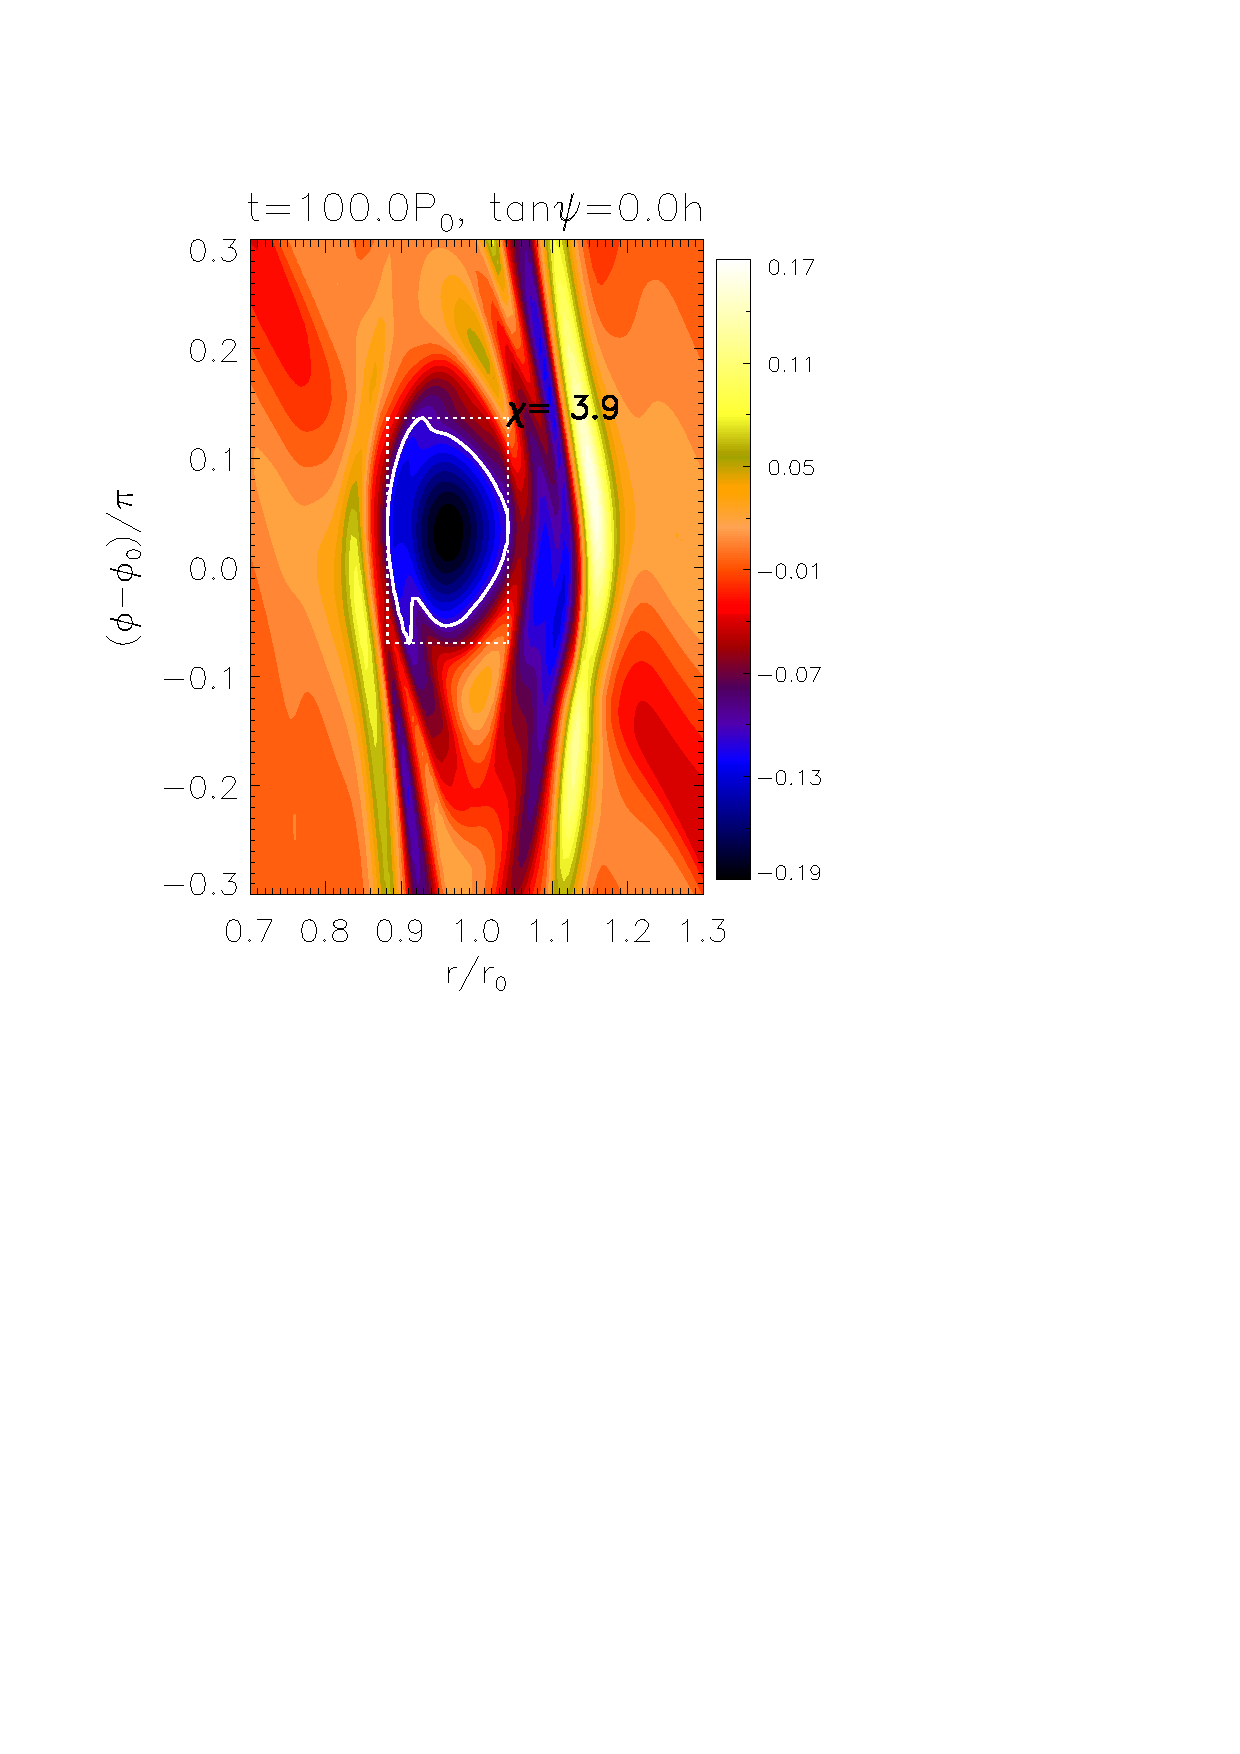
\includegraphics[scale=.43,clip=true,trim=2.3cm
     0.0cm 0cm
     0.99cm]{figures/vdamp2_vort010}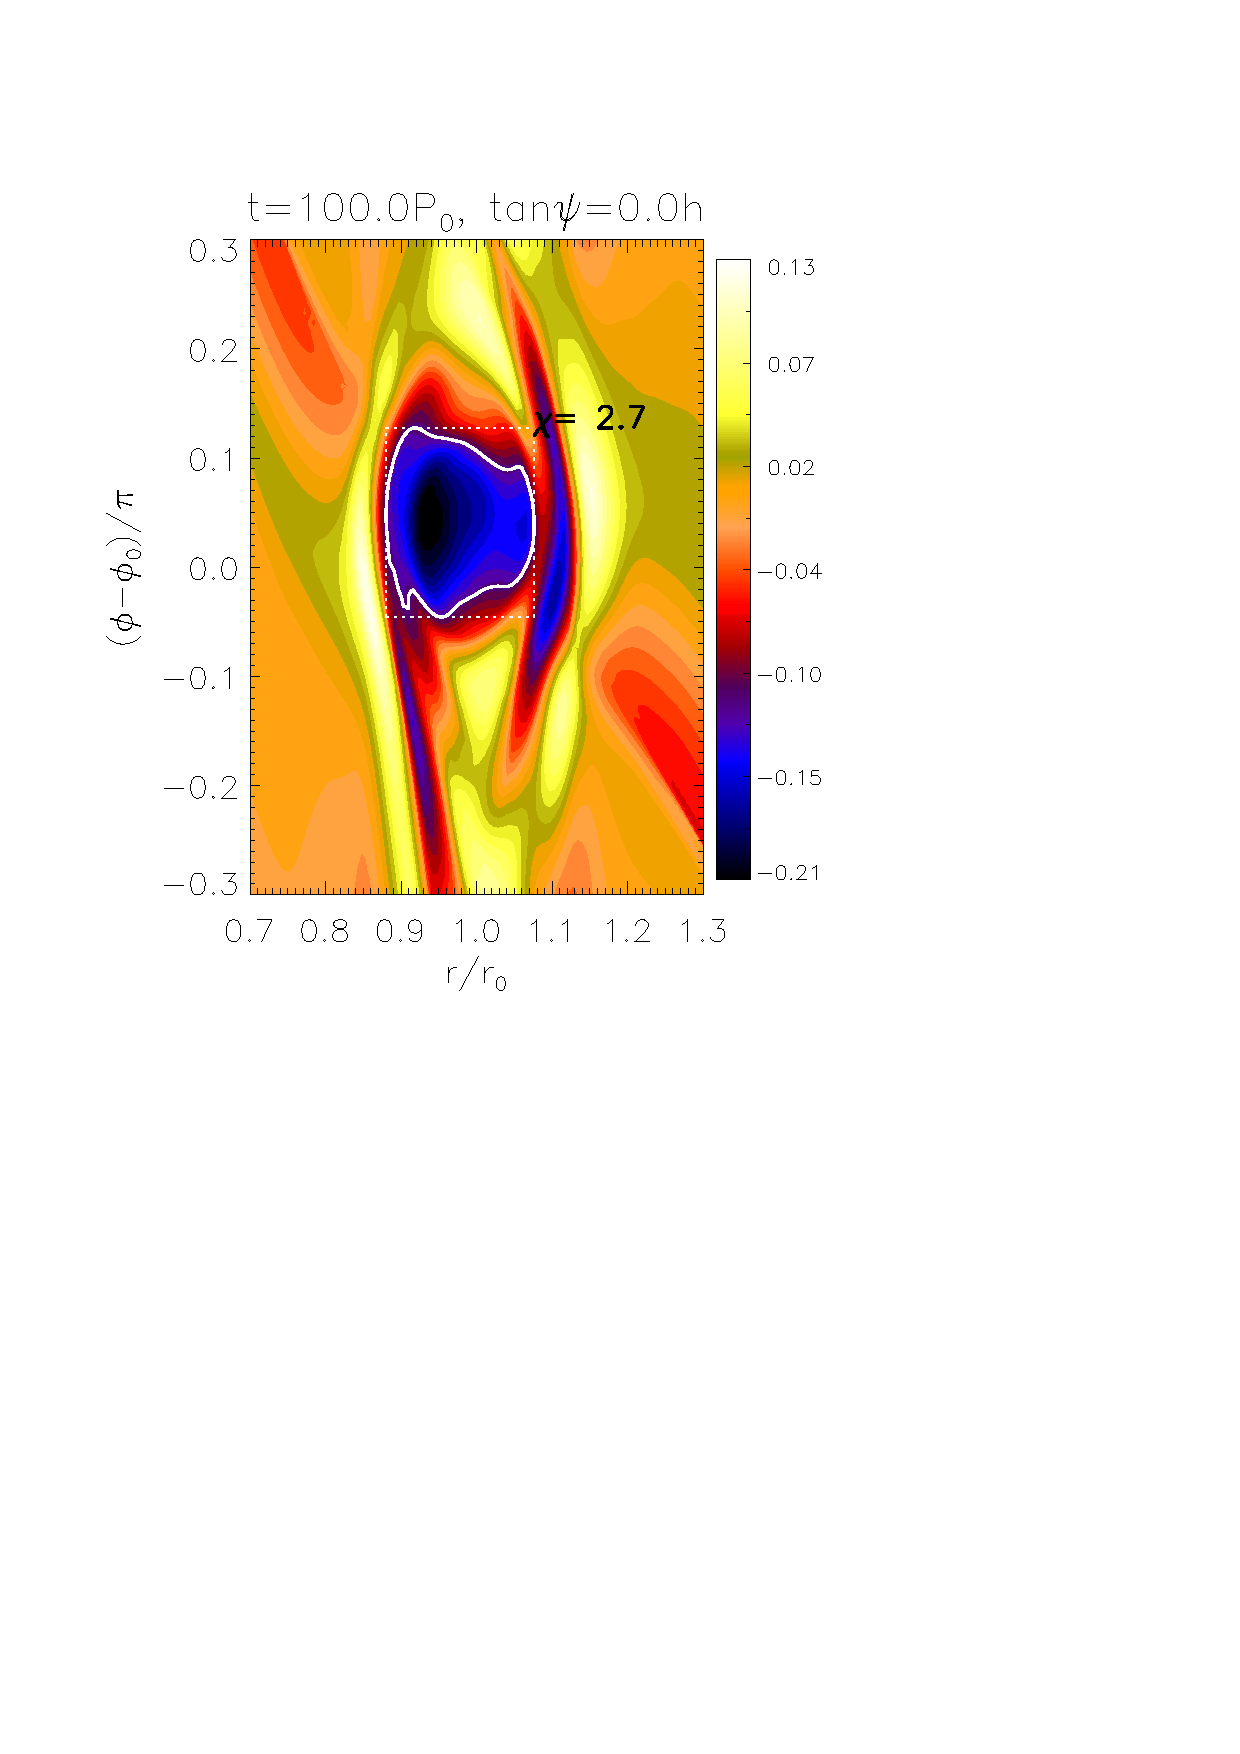
\includegraphics[scale=.43,clip=true,trim=2.3cm 
     0.0cm 0cm
     0.99cm]{figures/vdamp3_vort010}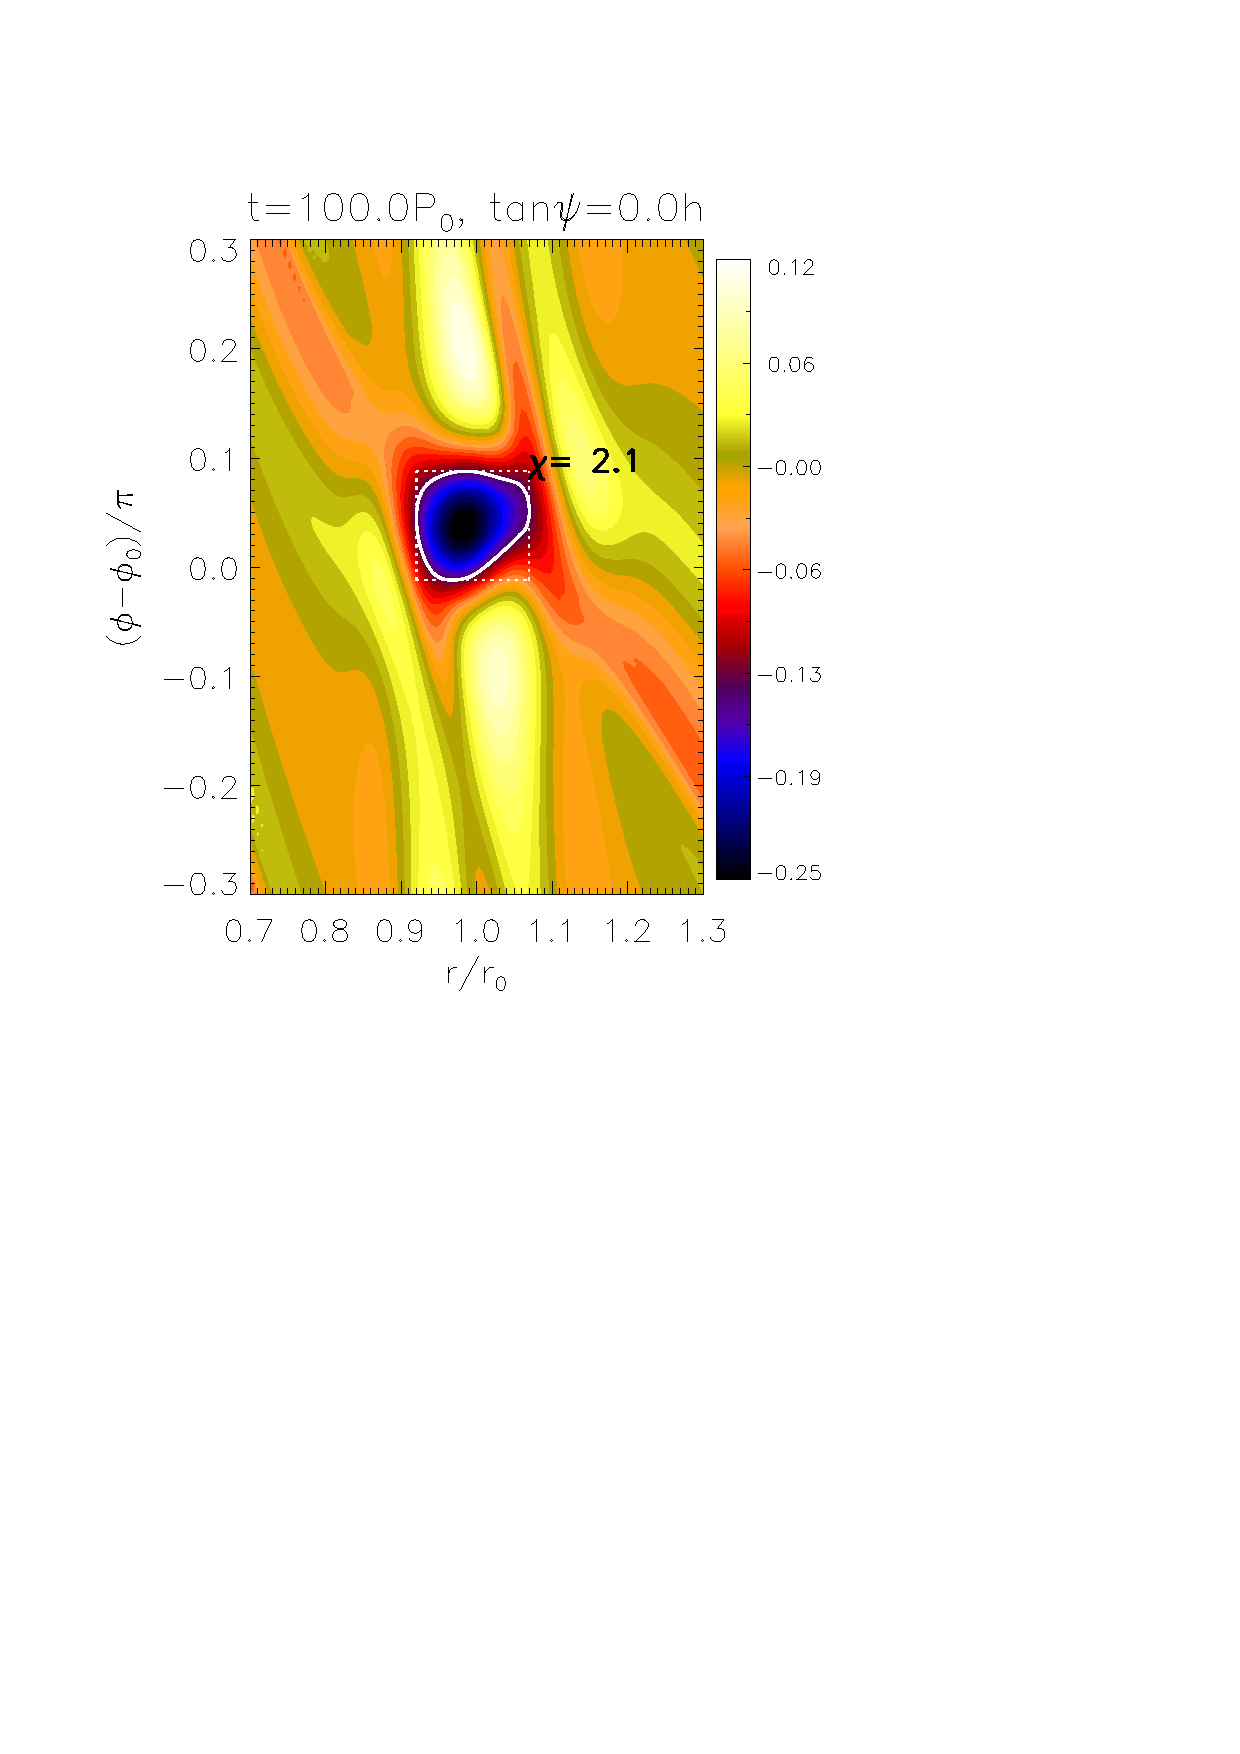
\includegraphics[scale=.43,clip=true,trim=2.3cm
     0.0cm 0cm
     0.99cm]{figures/vdamp0_nu4_vort010}
   \caption{Vortex formation in viscous discs initialised with
     a density bump at unit radius. Snapshots are taken at $t=100P_0$. The
     thickness of the viscous layer increases from left to 
     right: case V0, V1, V2 and V3.   
     Top: non-axisymemtric density field at the midplane
     $\Delta\rho(z=0)$. Bottom: midplane Rossby number
     $Ro(z=0)$. Here, $\phi_0$ is the azimuth of $\max[\Delta\rho(z=0)]$. 
     \label{vdamp0}
   }
\end{figure*}

%The top row of Fig. \ref{vdamp0} shows that layered viscosity has a
%non-trivial effect on $\Delta\rho$ in the 
%non-linear regime. $|\Delta \rho|$ increases
%from case V0 to V1, then decreases from cases V1 to V3 (but aquires a
%more global distribution). The dominant azimuthal wavenumber also
%increase: vortices do not readily merge in case V2 and V3. 

The effect of layered viscosity in the non-linear regime is more
complicated. The bottom row of Fig. \ref{vdamp0} compares the Rossby number
associated with the over-densities. Thickening the viscous 
layer decreases the vortex aspect ratio. Since their widths remain
at $\sim 2H_0$, the vortices become smaller with increasing
viscosity. This is partly attributed to fewer vortex merging
events having occured as viscosity is increased, which 
usually results in larger but weaker vortcies (smaller
$|Ro|$). If merging is resisted then each vortex can grow individually.  
Strangely, vortices become stronger  (more negative $Ro$) as viscosity
is increased. 

Fig. \ref{bump_energy} compares the perturbed kinetic energy for 
cases B0, V0 and V1; which are all dominated by a single vortex in 
quasi-steady state. We compute $W_1$ and compare its
average over the disc atmosphere and over the 
disc bulk. There is only a minor difference between the
perturbed kinetic energy densities between the disc bulk and
atmosphere, even in case V1 where the kinematic viscosity in the two
regions differ by a factor $\sim10^2$. This suggests that the
vortex evolves two-dimensionally. 

The energy perturbation in case B0 and V0 are both subject to
slow decay \citep[a result also observed by][]{meheut12}.  
By contrast case V1, which includes a high viscosity layer, does
\emph{not} show such a decay. We discuss this counter-intuitive result
below.  

%This suggests that
%viscosity could in fact strengthen the perturbation. 

\begin{figure}
  \centering
  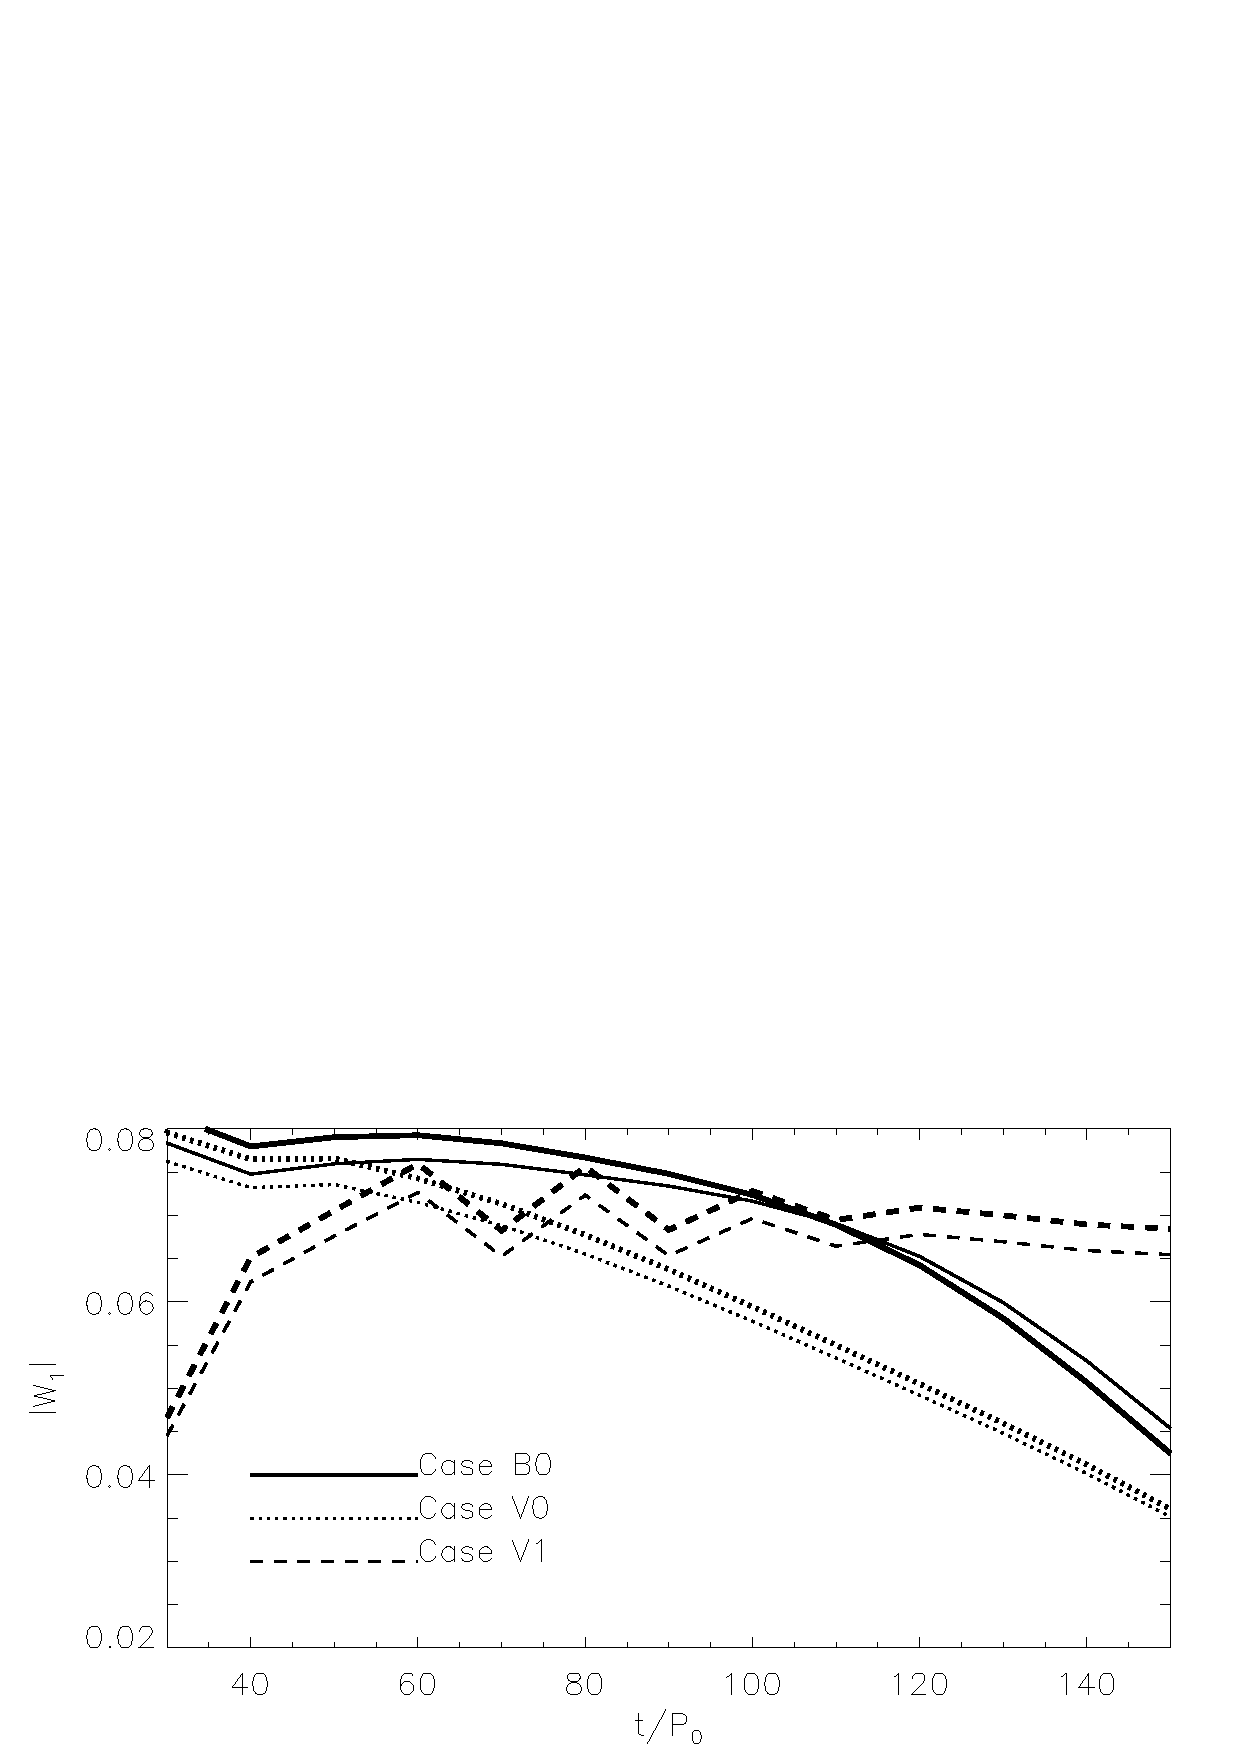
\includegraphics[width=\linewidth]{figures/pdisk_kerz_cases_bump}
  \caption{The $m=1$ component of the kinetic energy density, averaged
    over $r\in[0.8,1.2]r_0$, for the inviscid case B0 (solid), low
    viscosity case V0 (dotted) and a layered viscosity case V1 (dashed). 
    For each, the contribution 
    averaged over the disc atmosphere ($\tan{\psi}\in[0,0.5]h$, thin
    lines) and over the
    disc bulk ($\tan{\psi}\in[0.5,2.0]h$, thick lines) are plotted
    separately. 
    \label{bump_energy}}
\end{figure}

%%%%%%%%%%%%%%%%%%%%%%%%%%%%%%%%%%%%%%%%%%%%%%%%%%%%%%%%%%%%%%%%%%%%


\subsection{Order of magnitude comparison of timescales}
%The observation of stronger vortical structures (more negative $Ro$
%and smaller vortex aspect-ratio) with increasing
%viscosity is unexpected, since one normally expects viscosity to
%smooth out the flow. Here, we attempt to rationalise this
%result by comparing key timescales relevant to the problem. 

The characteristic spatial scale of the background density bump and of
the RWI is the local scale-height $H$, so the associated
viscous timescale is    
\begin{align}
  t_\nu = \frac{H^2}{\nu}\sim \frac{h^2}{\hat{\nu}\Omega}. 
\end{align}
The linear instability growth timescale is
\begin{align}
  t_\mathrm{RWI} = \frac{1}{\epsilon \Omega},
\end{align}
where $\epsilon$ is found from numerical simulations.   
The ratio of these timescales is
\begin{align}
  \frac{t_\nu}{t_\mathrm{RWI}} \sim \frac{\epsilon h^2}{\hat{\nu}}.
\end{align}
Table \ref{artificial_bump} indicates $\epsilon \sim 0.1$. 
Inserting $h=0.1$ and $\hat{\nu}=10^{-4}$ gives $t_\nu \sim 10
t_\mathrm{RWI}$. Thus viscosity damping is slower than linear
growth, even for the highest viscosity values we consider. 
Consequently the linear RWI is unaffected by viscosity. 

\cite{meheut13} argued that $t_\mathrm{RWI}$ is also the vortex
turn-over time $t_\mathrm{turn}$ when the instability saturates and
the linear phase terminates. Then 
$t_\nu\sim 10 t_\mathrm{turn}$, implying viscous effects 
are unimportant over one turn-over time. 
However, if we estimate a vortex turn-over time as $t_\mathrm{turn}
\sim 2\pi/|Ro|\Omega$ then $t_\nu\sim (h^2|Ro|/2\pi\hat{\nu})t_\mathrm{turn}$.  
Inserting $h=0.1,\,\hat{\nu}=10^{-4}$ and $|Ro|=0.25$ (case V3) gives 
$t_\nu \sim 4t_\mathrm{turn}$. Therefore, depending on the vortex shape, 
$t_\nu$ may not be much larger than $t_\mathrm{turn}$. 

In any case, our simulations span several local viscous timescales, 
$t_\mathrm{sim}\sim 10t_\nu $, so viscous damping should have taken
place, making the observation that $Ro$ becomes more negative as the 
viscous layer increases from case V0 to V3, a surprising
result. However, recall that we imposed a stationary, radially
structured viscosity profile consistent with a steady-state disc
containing a density bump. We suggest that for such setups, viscosity
attempts to restore the initial disc profile, i.e. the initial PV
minimum, thereby acting as a vorticity source.      

\subsection{Potential voritcity evolution}
The RWI is stronger for deeper PV minima \citep{li00}. We 
thus expect deeper PV minima to correlate with stronger vortices.   
For the above simulations the axisymmetric PV perturbation at the bump
radius is   
\begin{align}\label{vortensity_pert}
  \left.\frac{\aziavg{\eta_z}(t=100P_0)}{\eta_z(t=0)}\right|_{R=r_0} - 1 = 
  \begin{cases}
    3.99  & \text{Case V0} \\
   3.03  & \text{Case V1} \\
   2.24  & \text{Case V2} \\
   1.71  & \text{Case V3} \\
  \end{cases}.
\end{align} 
(This value is 4.92 for the inviscid case B0.) The PV 
perturbation is positive, thus the initial PV minimum is weakened
by the vortices \citep{meheut10}. This effect
diminishes with increasing viscosity. One contributing factor 
is the reduction in linear growth rate (Table 
\ref{artificial_bump}), implying the  
instability saturates at a smaller amplitude \citep{meheut13}. This  
is expected to weaken the background axisymmetric structure to a lesser
extent. However, the imposed viscosity profile may also actively
restore the initial density bump.     

When viscosity is small, the local viscous timescale $t_\nu$ is long compared to our
simulation timescale $t_\mathrm{sim}$. Then vortex formation weakens the PV minimum
with viscosity playing no role. Increasing viscosity eventually causes
$t_\nu<t_\mathrm{sim}$. This means that over the course of the
simulation, our spatially-fixed viscosity profile can act to recover the
initial PV minimum.  

We conjecture that in the non-linear regime there is competition 
between destruction of the background PV minimum by the 
vortices and reformation of the initial radial PV minimum by the
imposed viscosity profile. The latter should favour the RWI, since the
anti-cyclonic vortices are regions of local vorticity minima.  
 




\section{Vortex formation at planetary gap edges in layered
  discs}\label{disc-planet} 
The previous simulations, while necessary to isolate the effect of 
viscosity on the linear RWI, has the disadvantage that the radially
structured viscosity profile can act to source radial disc structure
in the non-linear regime. In this section, we employ a radially smooth
viscosity profile and use 
disc-planet interaction to
create the disc structure required for instability. We therefore expect viscosity to only
act as a damping mechanism. 

Vortex formation at gap edges is a standard result in 
2D and 3D hydrdynamical simulations of giant planets in low viscosity discs 
\citep{valborro07,lin10,lin11a,lin12}. The fact that this is due to
the RWI has been explicitly verified through linear stability
analysis %of planetary gap profiles produced from 2D simulations
\citep{valborro07,lin10}. Here, we simulate gap-opening giant planets
in 3D discs where the kinematic viscosity varies with height above the
disc midplane. Our numerical experiments are similar in spirit to
those performed by \cite{pierens10}, but our focus here is gap
stability in a layered disc. 
 
\subsection{Radially smooth viscosity profile for disc-planet
  interaction}\label{planet_visc_mode} 
Using the same notation as \S\ref{visc_model}, we impose a viscosity
profile $\hat{\nu}$ such that 
\begin{align}\label{planet_visc_profile}
  \hat{\nu}\Sigma_i(R)=
  \hat{\nu}_0\left[1+Q(\psi)\right]\Sigma_i(r_0)   
\end{align}
We have set the dimensionless argument in Eq. \ref{step} to
$\zeta=\psi$. Recall $\psi=\pi/2-\theta$ is the angular height away from the midplane. 
The viscosity increases from its floor value $\hat{\nu}_0$ by a factor
$A_\nu$ for $\psi > \zeta_\nu$. So the viscous layer is 
a wedge in the meridional plane, which conveniently fits into our
spherical grid. %The floor viscosity is $\hat{\nu}_0=2.5\times 10^{-7}$
%or $\hat{\nu}_0=10^{-6}$. 
The angluar thickness of the viscosity
transition is fixed to $\Delta\zeta_\nu =
0.2h$. Fig. \ref{planet_visc2d} gives an example of this  
viscosity profile. 

\begin{figure}
  \centering
  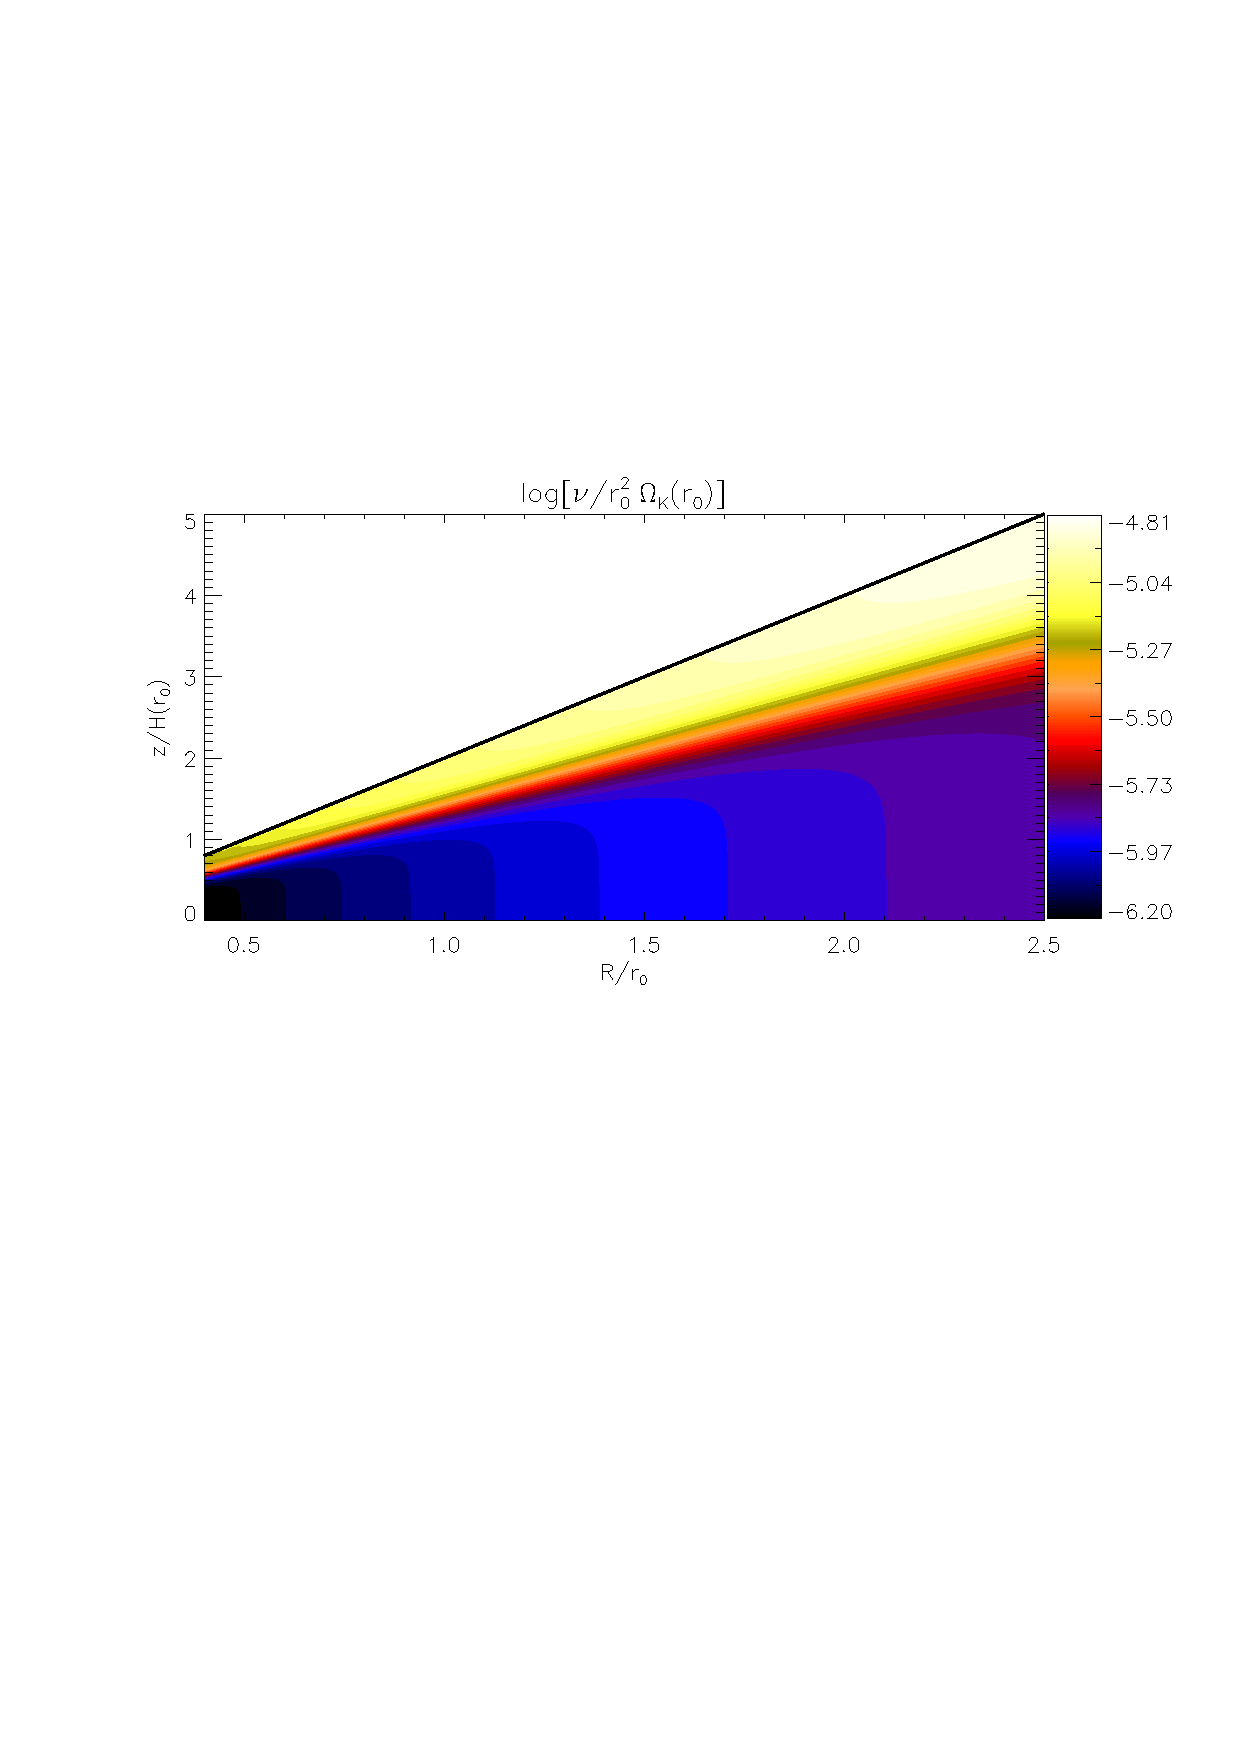
\includegraphics[width=\linewidth]{figures/pdisk_visc2d_planet}
  \caption{Example of the viscosity profile
    imposed in disc-planet simulations
    (Eq. \ref{planet_visc_profile}).  
    For a disc with constant aspect ratio, the viscous
    layer occupies a constant number of scale heights across the
    radial range. This specific plot corresponds to case P1, so the
    viscous layer (yellow-white colours) always occupies the uppermost
    $H$ at each cylindrical radius. 
    The solid line delineates the upper boundary of the computational
    domain. 
    \label{planet_visc2d}}
\end{figure}

\subsection{Disc-planet simulations} 
We simulate locally isothermal discs with constant aspect-ratio
$h=0.05$ (by choosing $q=1$), vertical extent $n_h=3$ scale-heights 
and radial extent $[\rin,\rout]=[0.4,2.5]r_0$. Initially the surface density is smooth
($A=1$) with zero meridional velocity ($v_r=v_\theta=0$). 
%cylindrical radial velocity is given by
%Eq. \ref{init_vr}. 
The standard resolution is $(N_r, N_\theta,
N_\phi)=(256, 96, 768)$, corresponding to $6,\,32,\,6$ 
cells per $H$ along the $r,\theta,\phi$ directions at the reference
radius. We apply a damping rate $\hat{\gamma}=2$ with the reference
velocity field $\bm{v}_\mathrm{ref}=(0,0,v_\phi)$ in spherical
co-ordinates.   

We insert into the disc a planet of mass  
$M_p=10^{-3}M_*$, which corresponds to a Jupiter mass planet if
$M_*=M_{\sun}$. The softening length for the planet potential is
$\epsilon_p=0.5r_h$. The planet potential is switched on 
smoothly over $t\in[0,10]P_0$. We note that the disc can be considered
as two-dimensional for gap-opening giant planets, because the Hill
radius $r_h$ exceeds the local scale-height $H$ ($r_h/H\simeq1.4$
in our cases).   

We remark that, apart from the viscosity prescription, the above
choice of physical and numerical parameter values are typical for
global disc-planet simulations \citep[e.g.][]{valborro06,mignone12}.    


%%%%%%%%%%%%%%%%%%%%%%%%%%%%%%%%%%%%%%%%%%%%%%%%%%%%%%%%%%%%%%%%%%%%%%%%%%%%%%%


\subsection{Results}
Table \ref{planet_sims} summarises the disc-planet simulations. 
%\subsubsection{Runs} 
The main simulations to be discussed are cases P0 --- P1, with a floor
viscosity of $\hat{\nu}_0=2.5\times10^{-7}$. 
The fiducial run P0 has $A_\nu=1$, i.e. no viscous layer, so 
$\hat{\nu}\sim 10^{-7}$ ($\alpha\sim 10^{-4}$) everywhere. 
The typical viscosity value adopted for disc-planet simulations,
$\hat{\nu}\sim 10^{-5}$ or $\alpha\sim 10^{-3}$, is known to surpress vortex formation
\citep{valborro07, mudryk09}. Thus vortex formation is expected for
case P0. For case P0.5 and P1 we set $A_\nu=100$ with transition angle $\zeta_\nu=2.5h$ and
$2h$, respectively, so the viscous layer with $\hat{\nu}\sim10^{-5}$
($\alpha\sim10^{-2}$) occupies the uppermost $0.5H$ and $H$ of the vertical
domain. Case P0R is case P0 restarted from 
$t=100P_0$ with the layered viscosity profile of case P1. 
 

\begin{table*}
  \centering
  \caption{Summary of disc-planet simulations. These runs employ the
    `wedge' viscosity model described by
    Eq. \ref{planet_visc_profile}. The thickness of the viscous layer
    is measured from the upper disc boundary. The $m=1$ mode amplitude was 
    averaged over the shell $r\in[1.2,1.6]r_0$ and over time 
    $t\in[t_\mathrm{max},200]P_0$, where $t_\mathrm{max}$ is when
    $\mathrm{max}(a_1)$ is attained. Case P0R employs the
    viscosity profile of P0 for $t\leq100P_0$, and that of P1 for 
    $t>100P_0$.\label{planet_sims}}
    \begin{tabular}{llllrrl}
      \hline\hline
      Case & $10^6\hat{\nu}_0$ & $A_\nu$ & visc. layer&
      $10^2\overline{a}_1$&$10^2a_{1,t=200P_0}$ & comment \\ 
      \hline
      P0     & 0.25  & 1            & 0     & 18.3  & 14.5 & single vortex
       by $t=130P_0$ and persists until end of sim.  \\ %doing HR
      P0.5   & 0.25  & 100          & $0.5H$ &  17.4  & 8.6& single vortex
      by $t=90P_0$ and persists until end of sim.\\ 
      P0R    & 0.25  & 1$\to$100    & $0\to H$& 10.1 & 2.5& single vortex
      by $t=130P_0$, disappears after $t=180P_0$ \\
      P1     & 0.25  & 100          & $H$    & 12.5  & 2.1 &single vortex
      by $t=80P_0$, disappears after $t=170P_0$ \\   %doing HR
      

      Pb0     & 1.0  & 1          & 0      & 9.2  & 5.4 &single vortex by $t=130P_0$, disappears
      vortex after $t=160P_0$   \\ %doing HR
      Pb0.5   & 1.0  & 10         & $0.5H$ & 7.3  & 3.0 &similar to Pb0     \\ 
      Pb1     & 1.0  & 10         & $H$    & 5.7  & 2.2   &single vortex
      by $t=120P_0$, disappears after $t=140P_0$   \\ %doing HR

      Pc0.5   & 1.0  & 100          & $0.5H$ & 4.2  &  2.3 &two vortices
      at $t\sim100P_0$, no vortices after $t\sim120P_0$   \\ %optional
      Pc1     & 1.0  & 100          & $H$    & 2.2 &  1.6 &two weak vortices at
      $t\sim60P_0$, no vortices after $t\sim 80P_0$\\ %optional  
      \hline
  \end{tabular}
\end{table*}

%other sims
%loc iso (q=1) with floor visc 1d-6, amp=100 and 10. HR for one of
%them. and visc-restart.  
%isothermal (q=0) with floor visc=1d-6, amp=100 and 10
%may need to add other columns nu_floor, nu_amp, q 

\subsubsection{Density evolution}%prob replace with nu_floor=1d-6,
                                %amp=10 sims

Fig. \ref{jup0_3h} compares the time evolution of the midplane density
perturbation $\delta\rho(z=0)$ for cases P0, P0.5 and P1. In 
all cases we observed the RWI with $m=4$ develops early on ($t\simeq20P_0$),
consistent with the limited effect of viscosity on the linear
instability, as found above.  

Comparing the no-layer case P0 to case P0.5 (viscous layer $0.5H$)
shows that a thin viscous layer has little effect on the
evolution of the unstable gap edge, except the vortex merging
time-scale is slightly altered. However, case P1 evolves quite
differently from case P0. While a single vortex does form at
$t\sim100P_0$ in case P1, it is \emph{transient}, having disappeared at the end of
the simulation. The final $m=1$ amplitude is about 3 times smaller
than that in case P0 (Table \ref{planet_sims}). This result is
significant because an upper viscous layer of 
thickness $H$ only occupies $\sim4\%$ of the total column density
in case P1, but the vortex is still destroyed. This suggests that vortex
survival at planetary gap edges requires low effective viscosity
throughout the vertical fluid column. 

\begin{figure*}
  \centering
  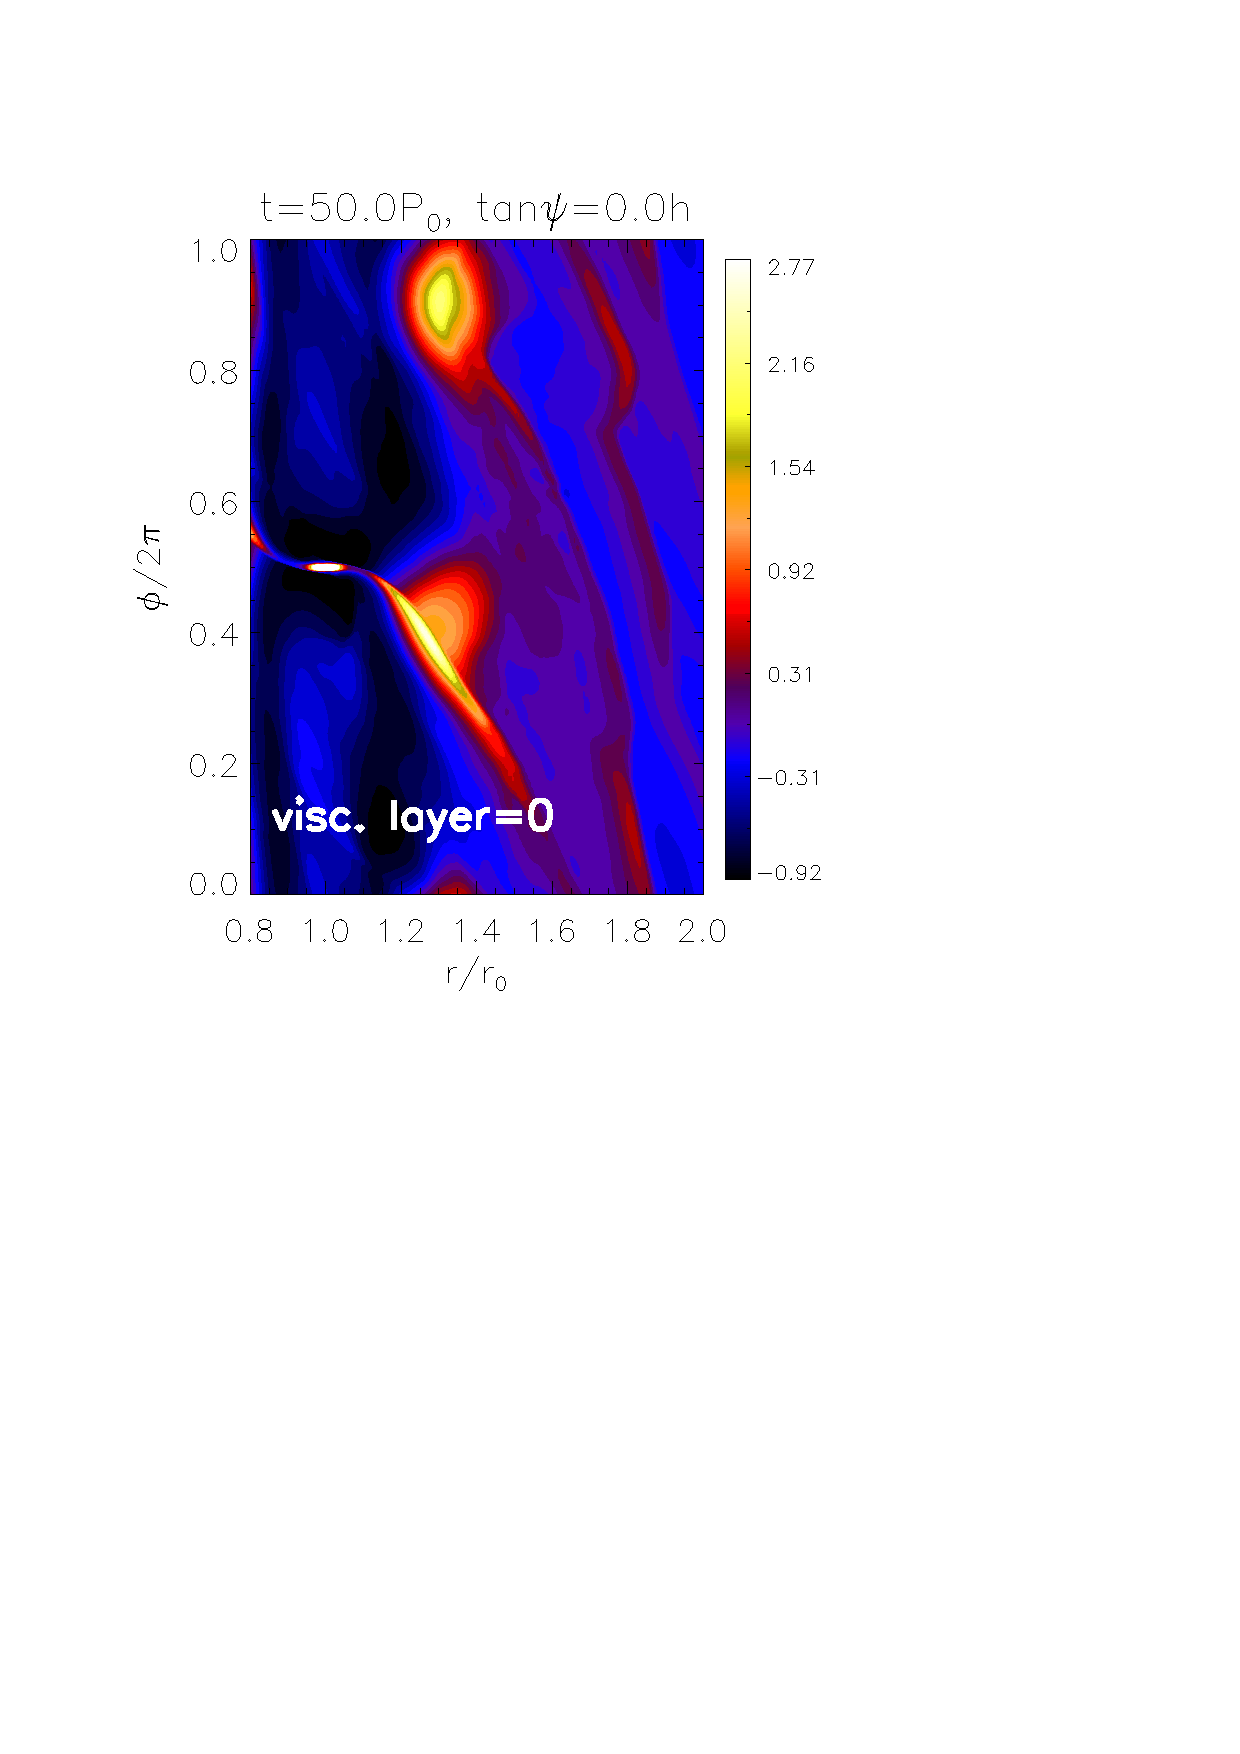
\includegraphics[scale=.43,clip=true,trim=0cm 1.84cm 0cm
    0cm]{figures/jup0_3h_pdisk_005}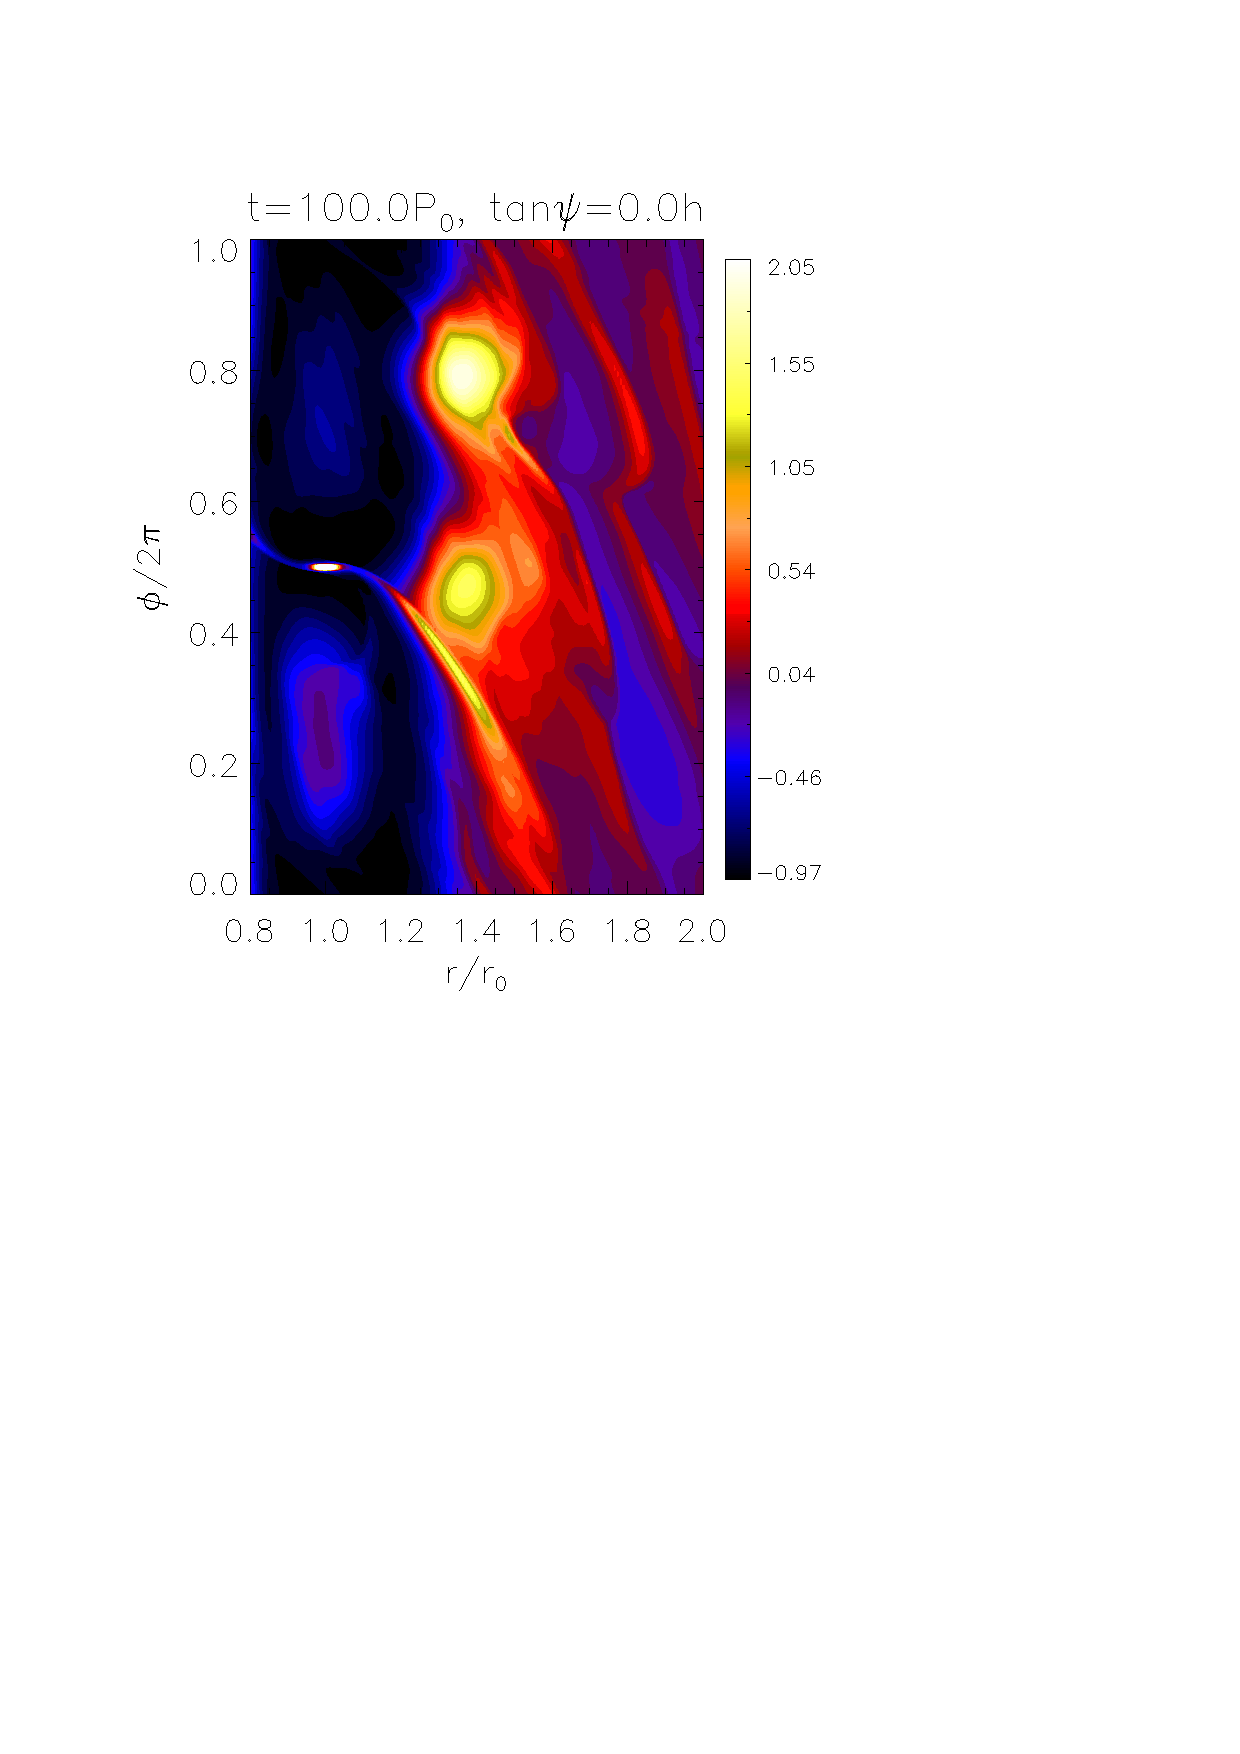
\includegraphics[scale=.43,clip=true,trim=2.3cm
    1.84cm 0cm 0cm]{figures/jup0_3h_pdisk_010}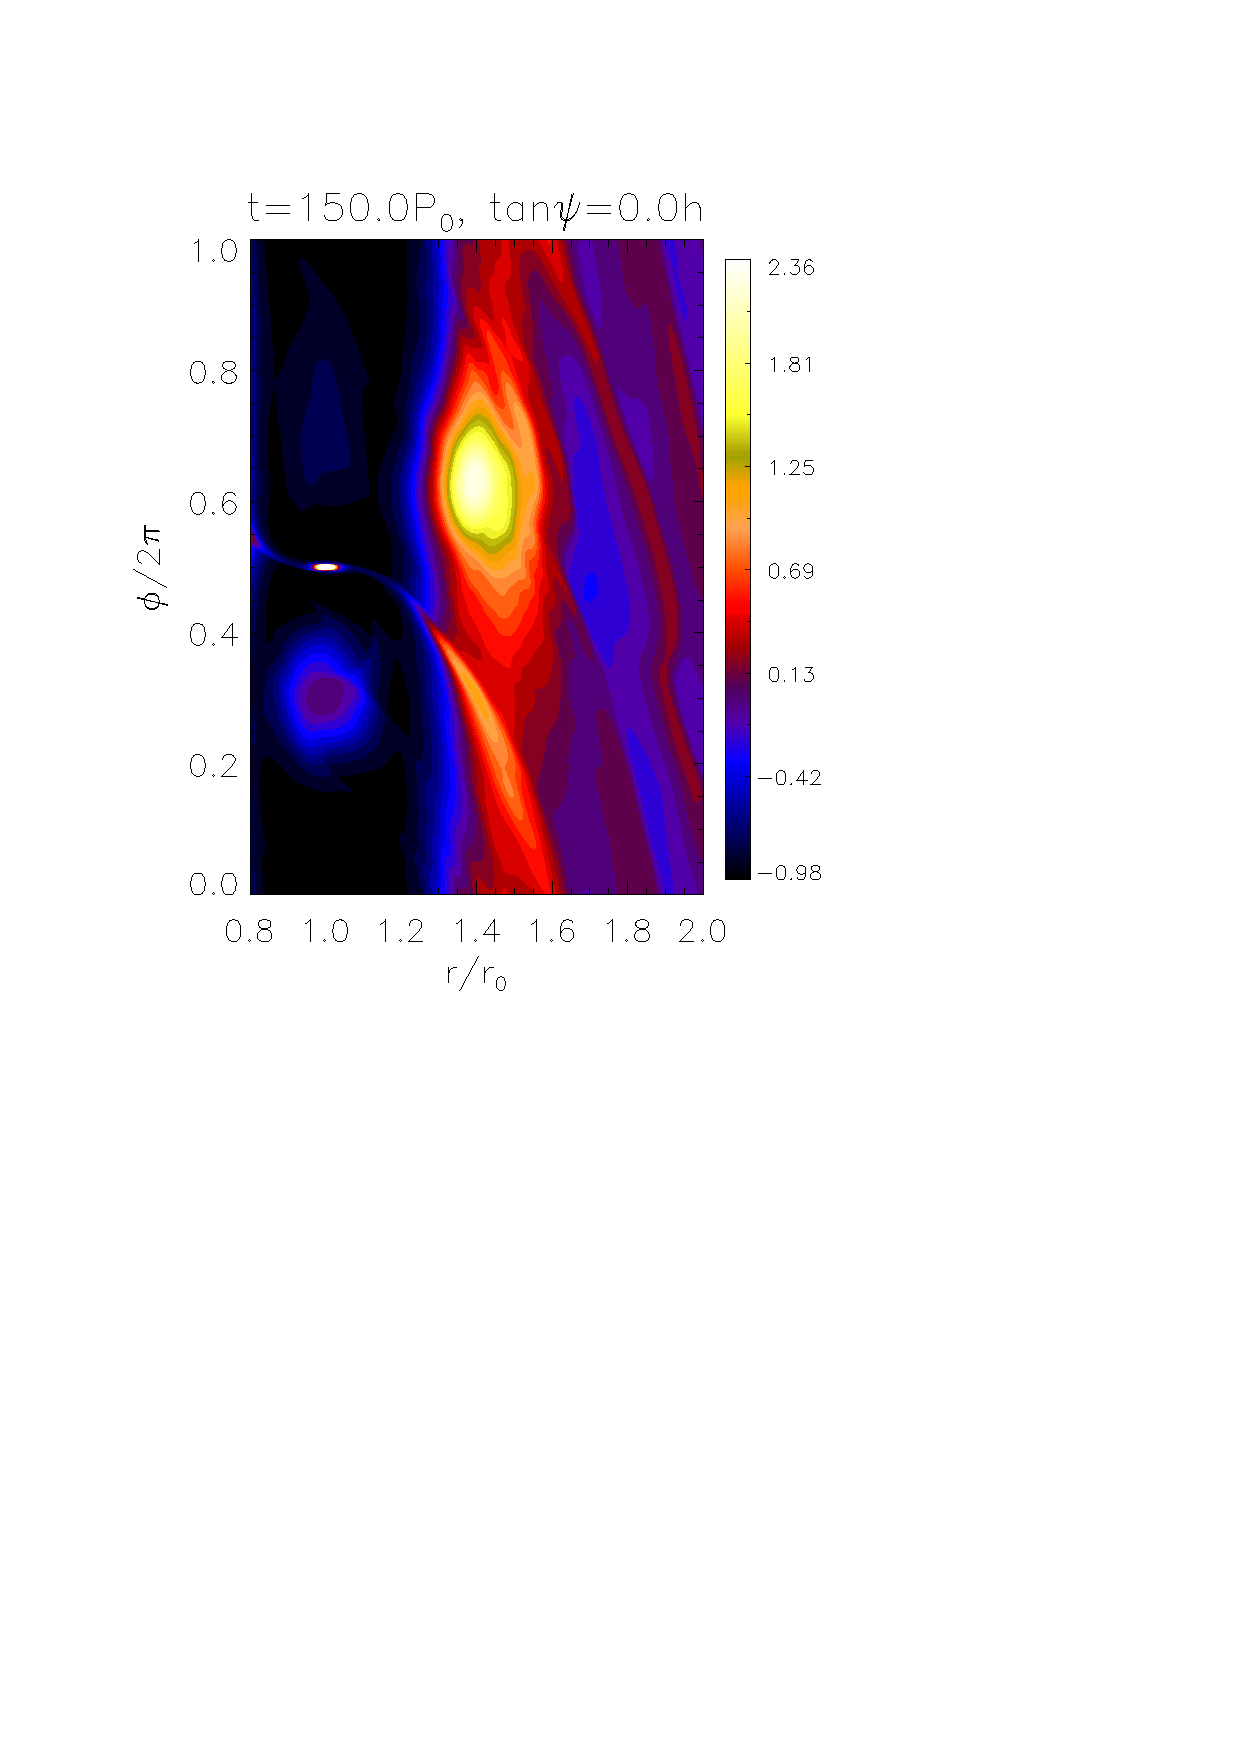
\includegraphics[scale=.43,clip=true,trim=2.3cm
    1.84cm 0cm 0cm]{figures/jup0_3h_pdisk_015}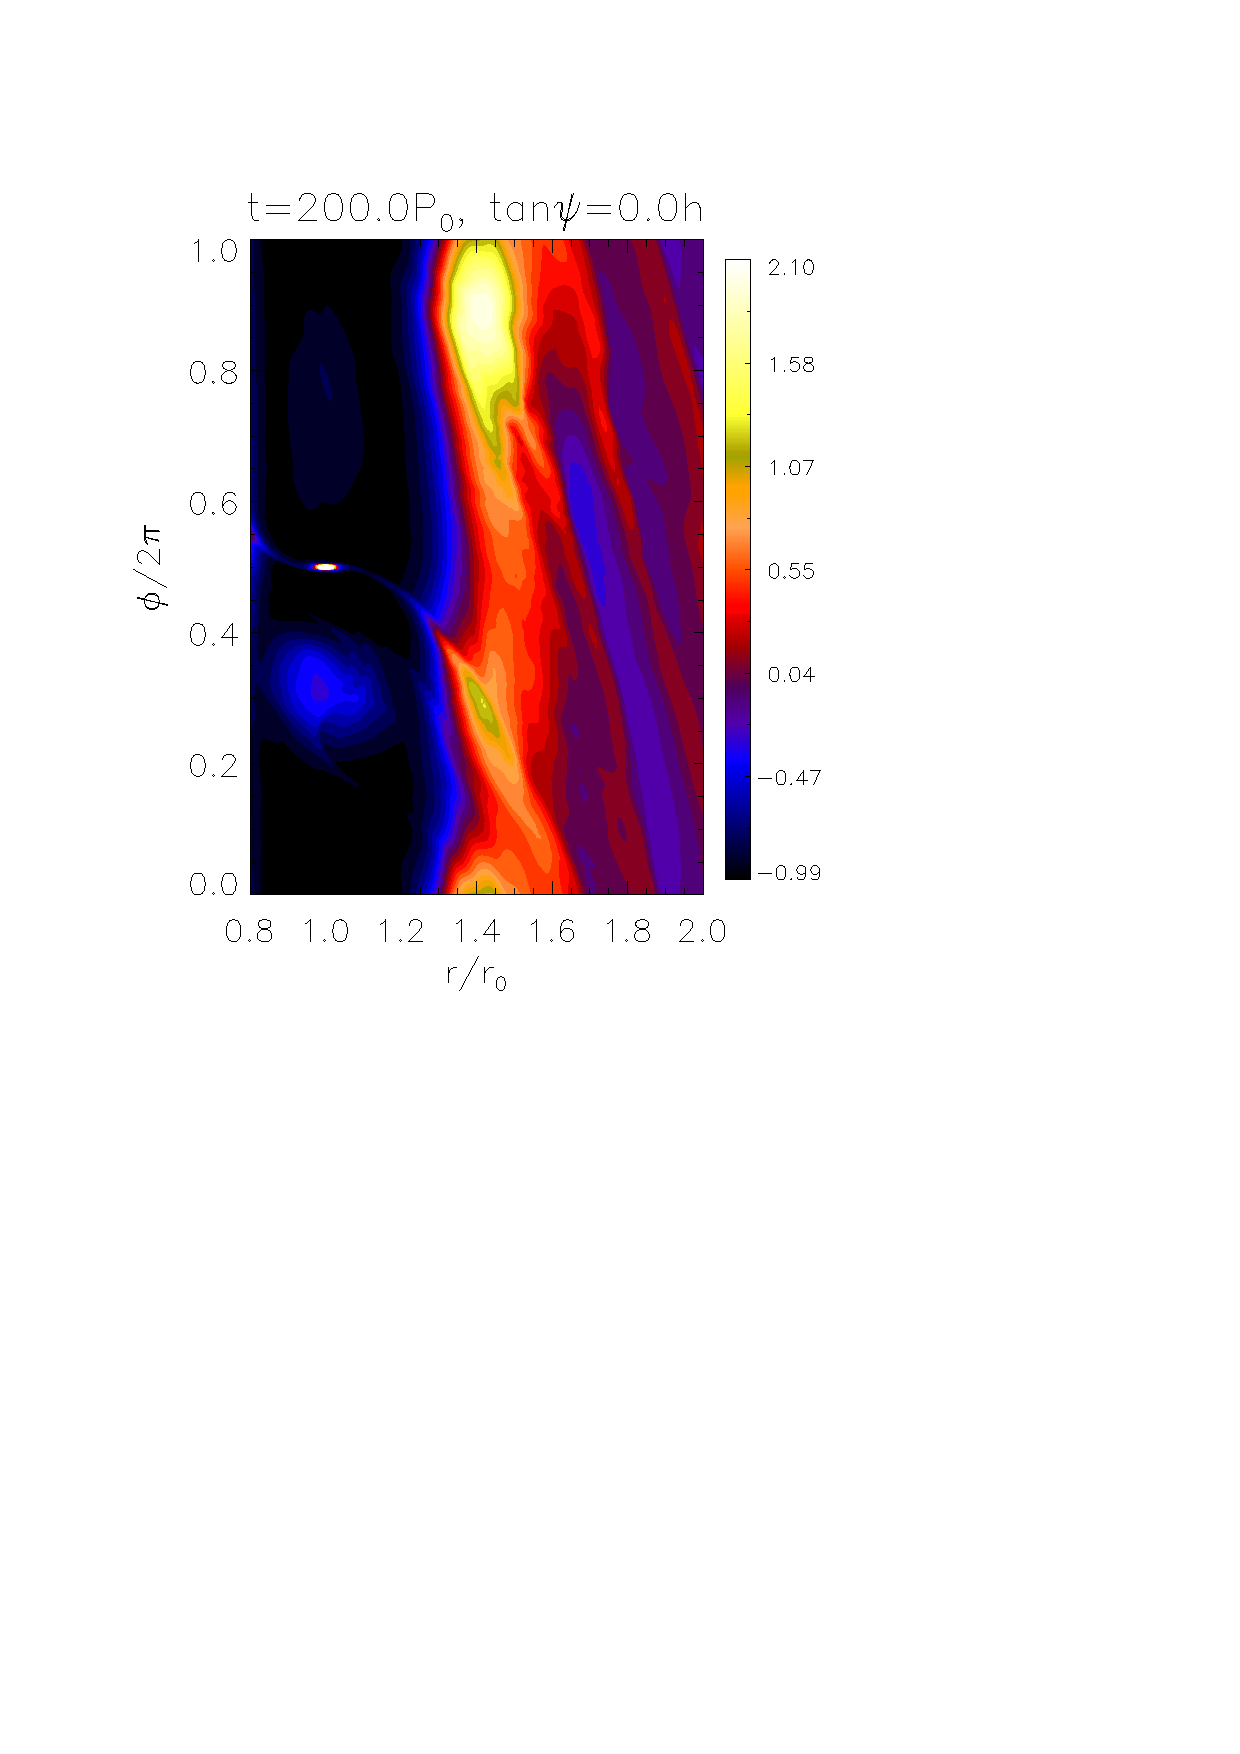
\includegraphics[scale=.43,clip=true,trim=2.3cm
    1.84cm 0cm 0cm]{figures/jup0_3h_pdisk_020}\\
%  \includegraphics[scale=.43,clip=true,trim=0cm 1.84cm 0cm
%    0.9cm]{figures/jup0d5_3h_pdisk_005.ps}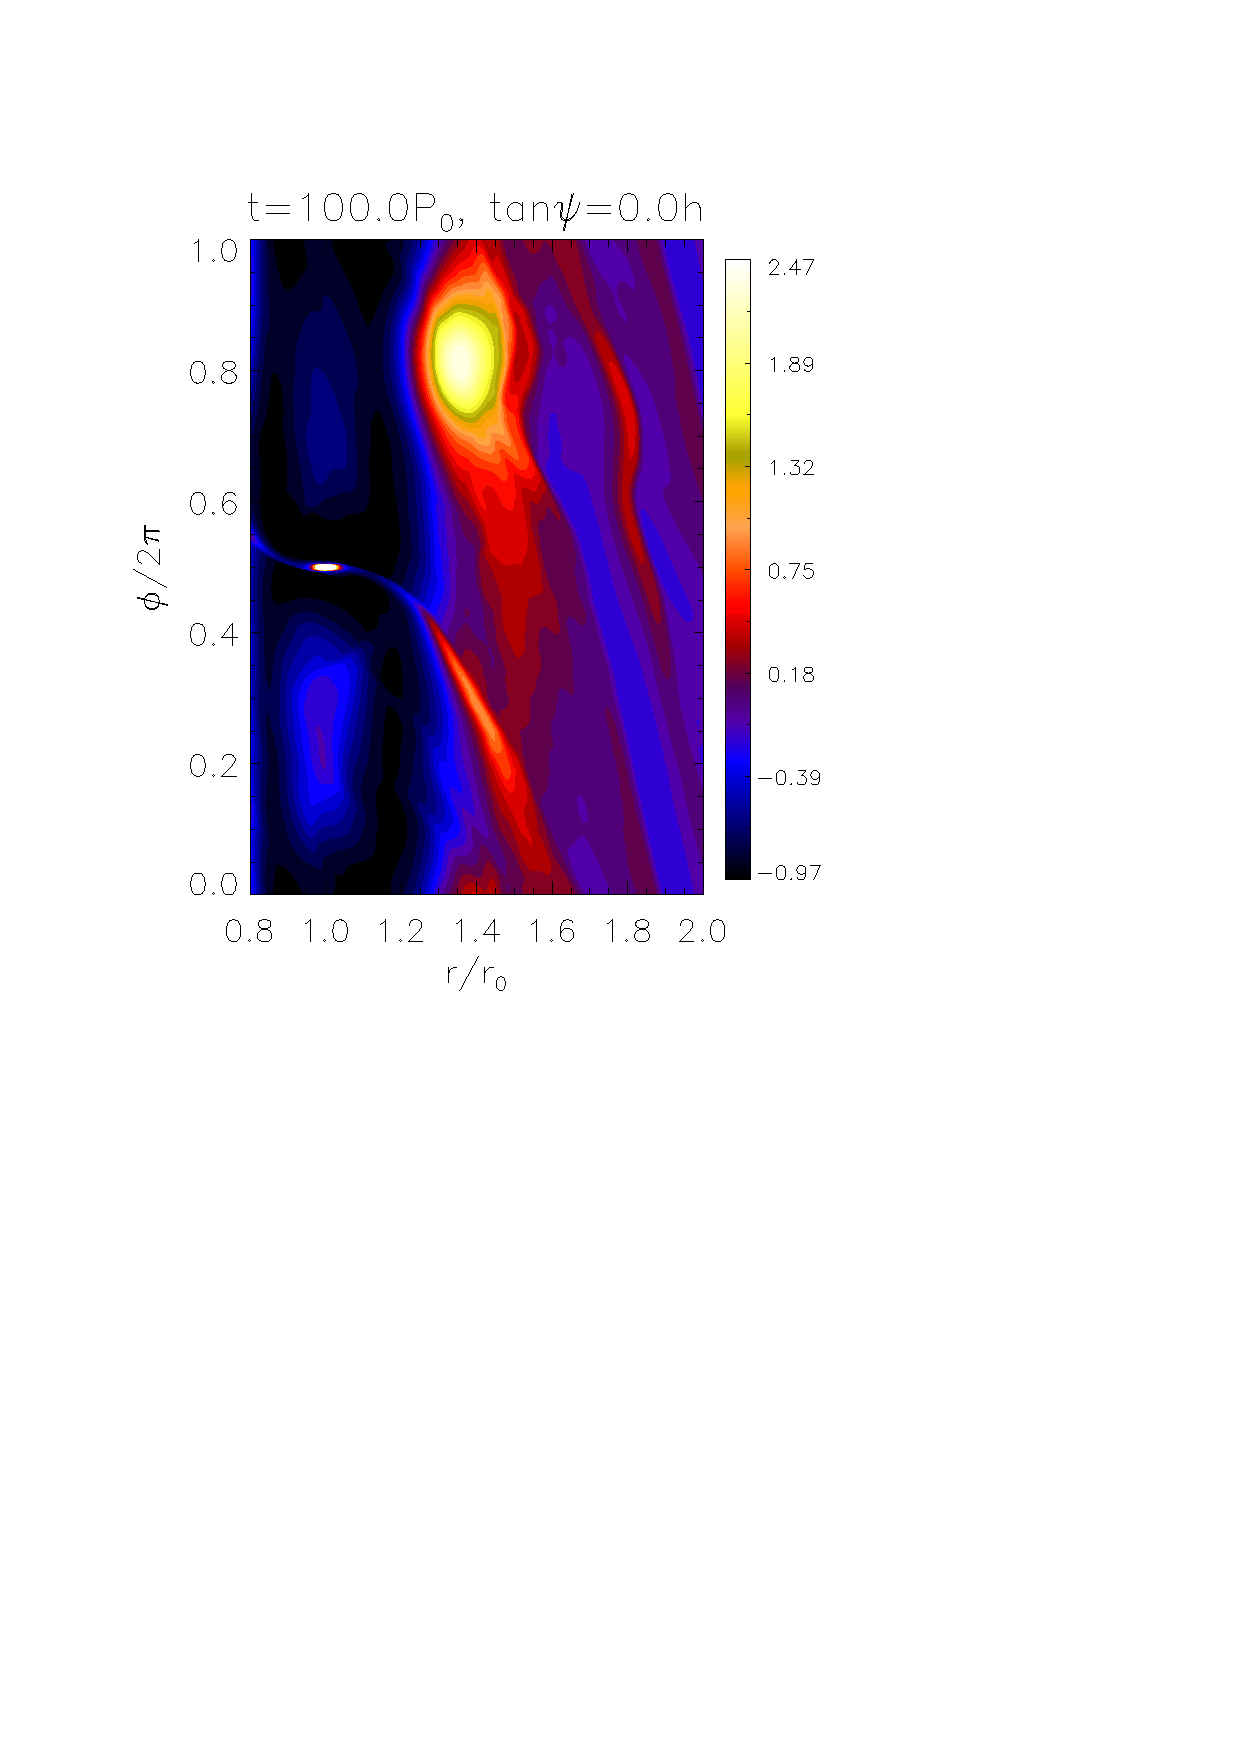
\includegraphics[scale=.43,clip=true,trim=2.3cm
%    1.84cm 0cm 0.9cm]{figures/jup0d5_3h_pdisk_010}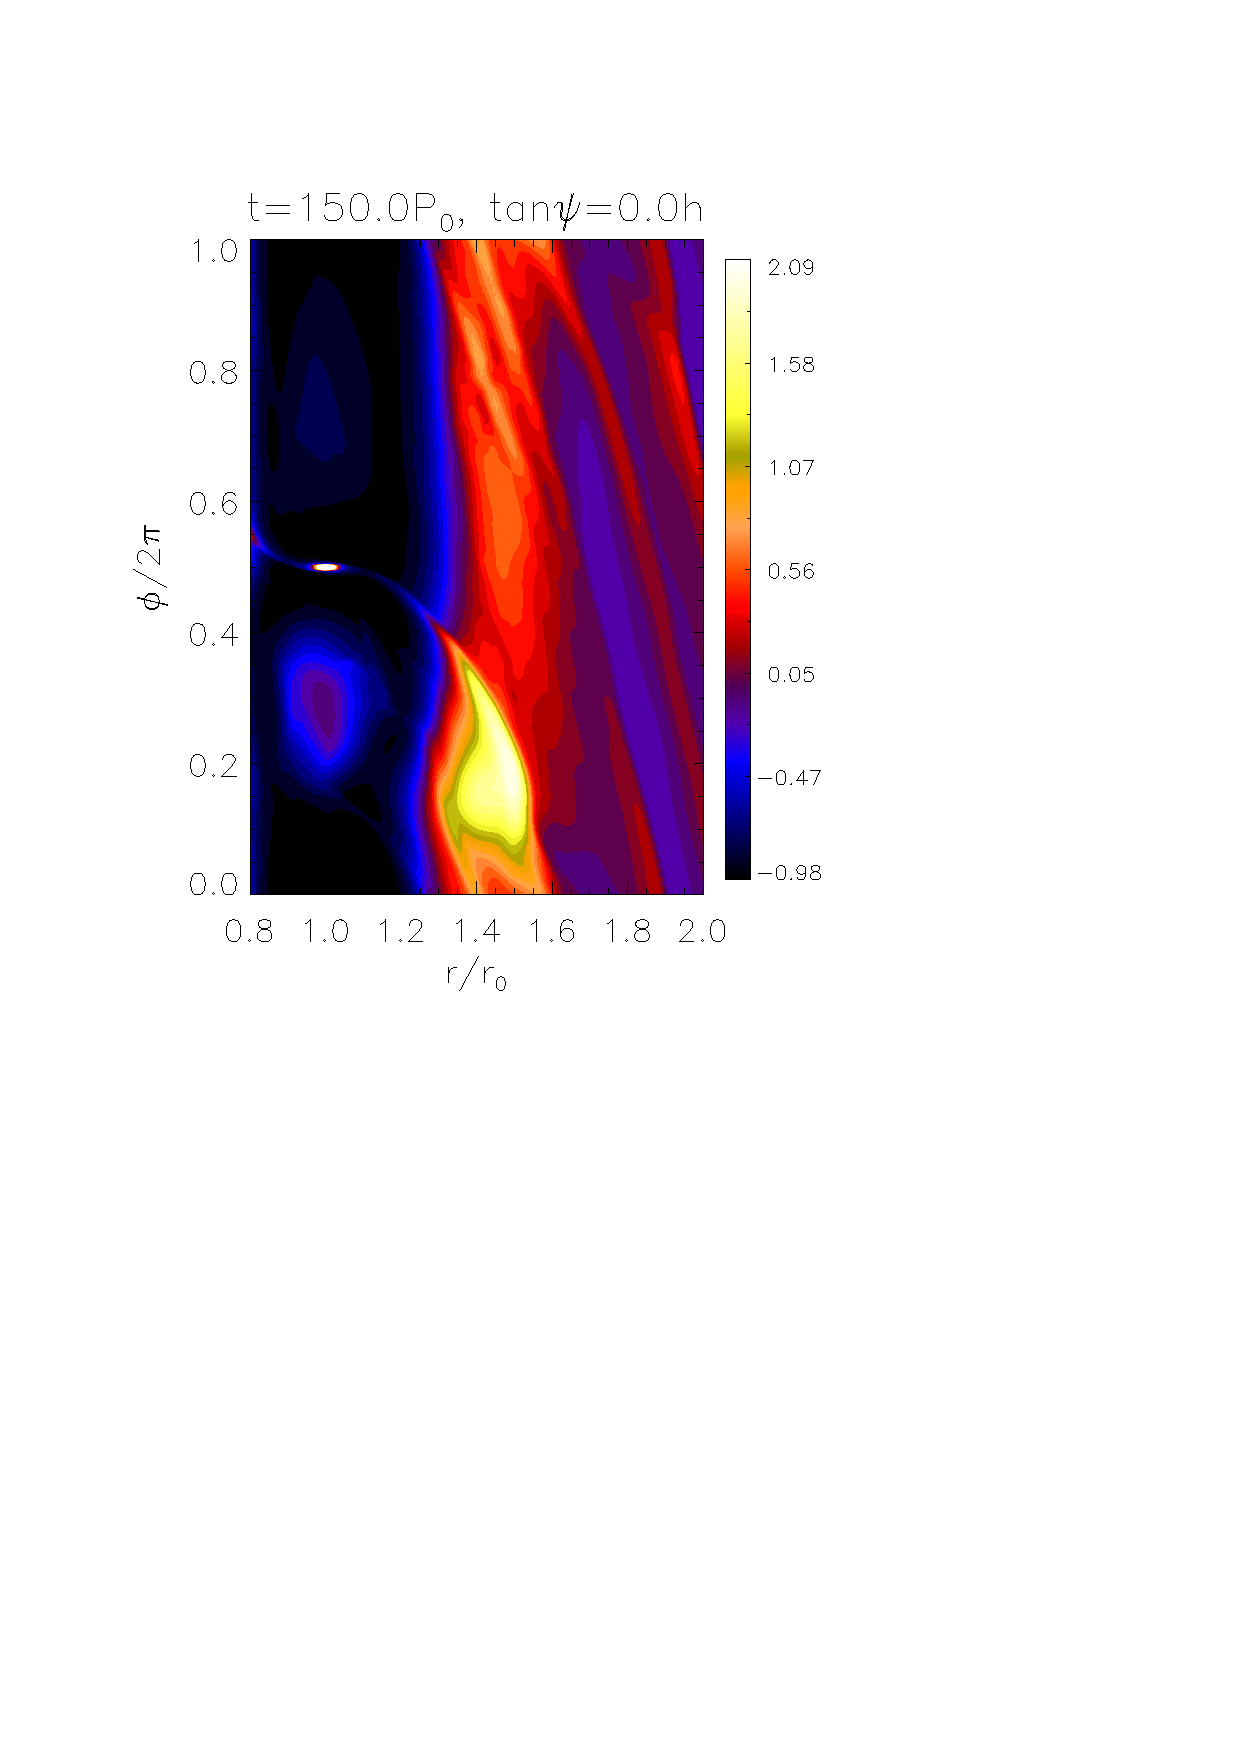
\includegraphics[scale=.43,clip=true,trim=2.3cm
%    1.84cm 0cm 0.9cm]{figures/jup0d5_3h_pdisk_015}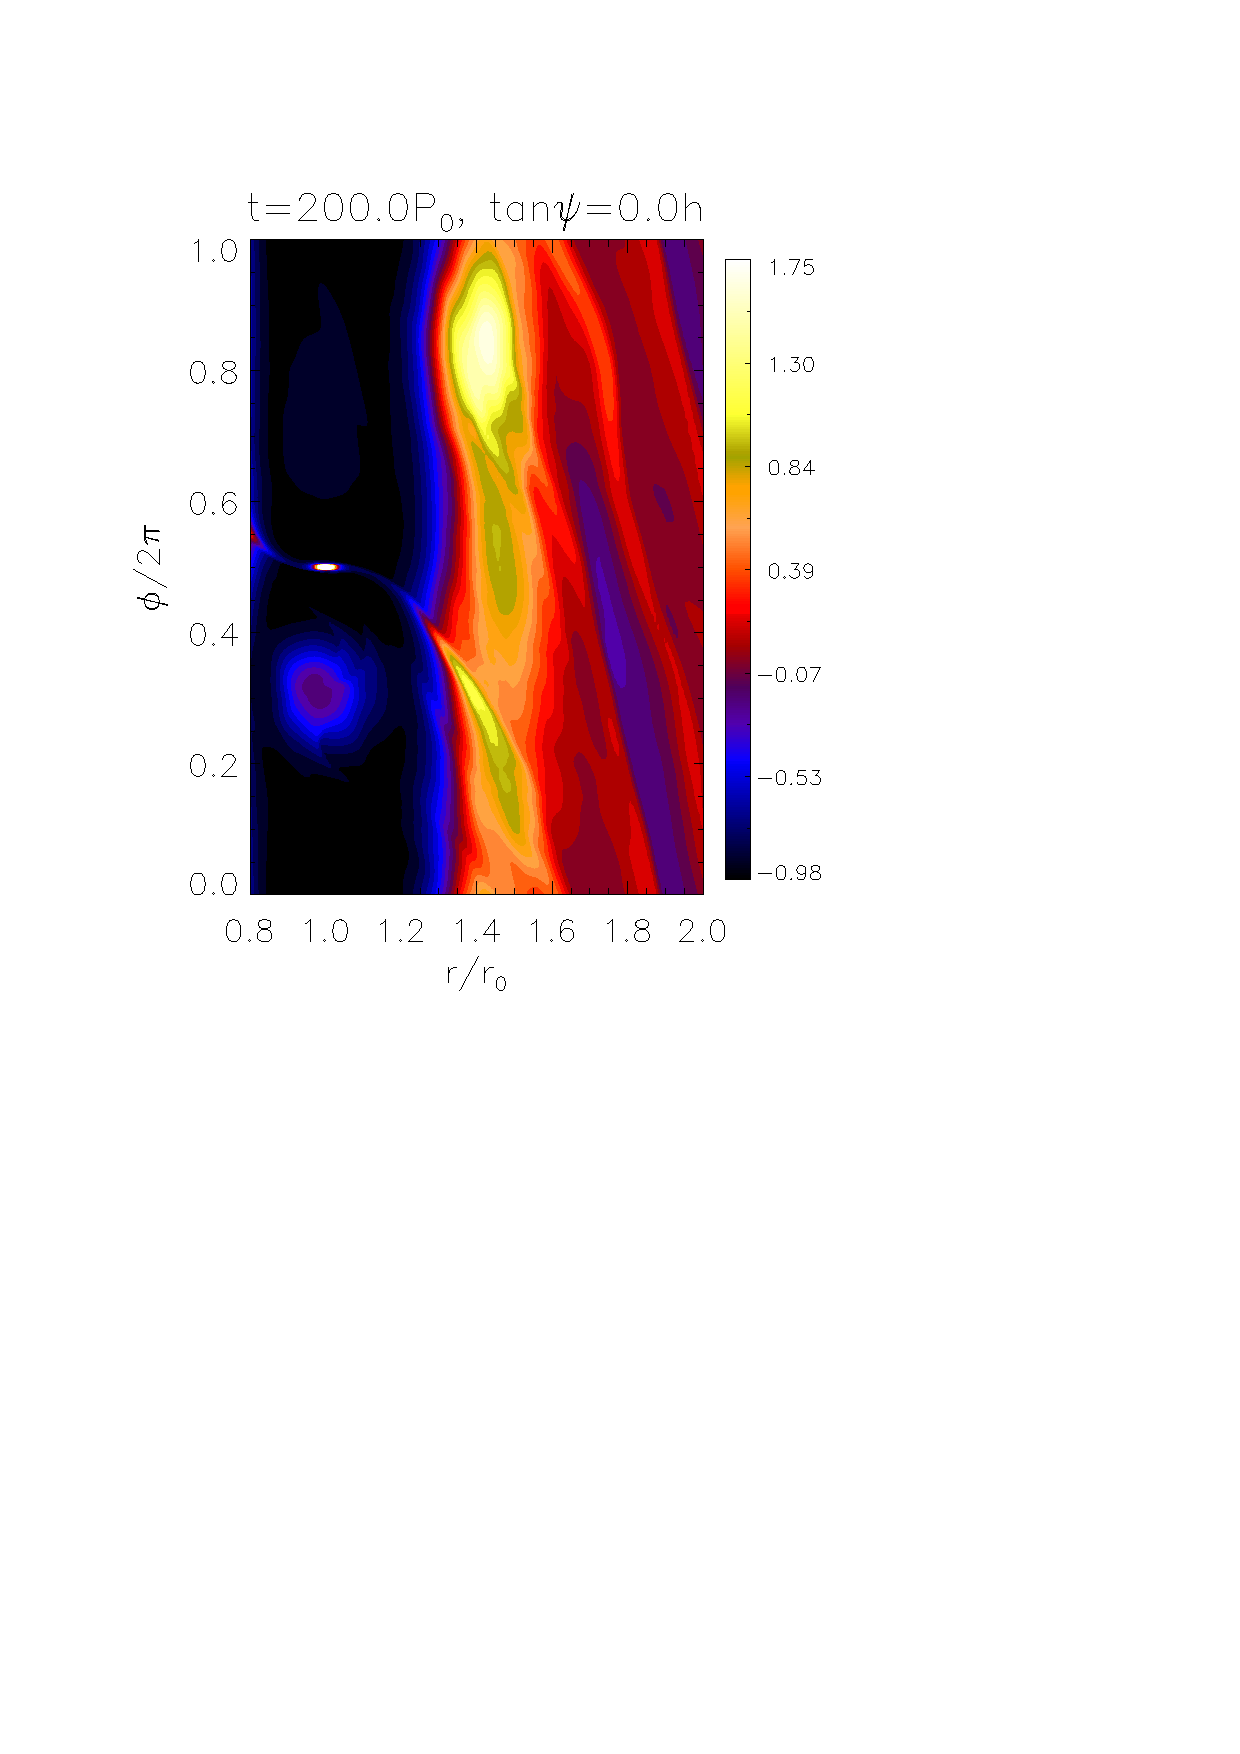
\includegraphics[scale=.43,clip=true,trim=2.3cm
%    1.84cm 0cm 0.9cm]{figures/jup0d5_3h_pdisk_020}\\
  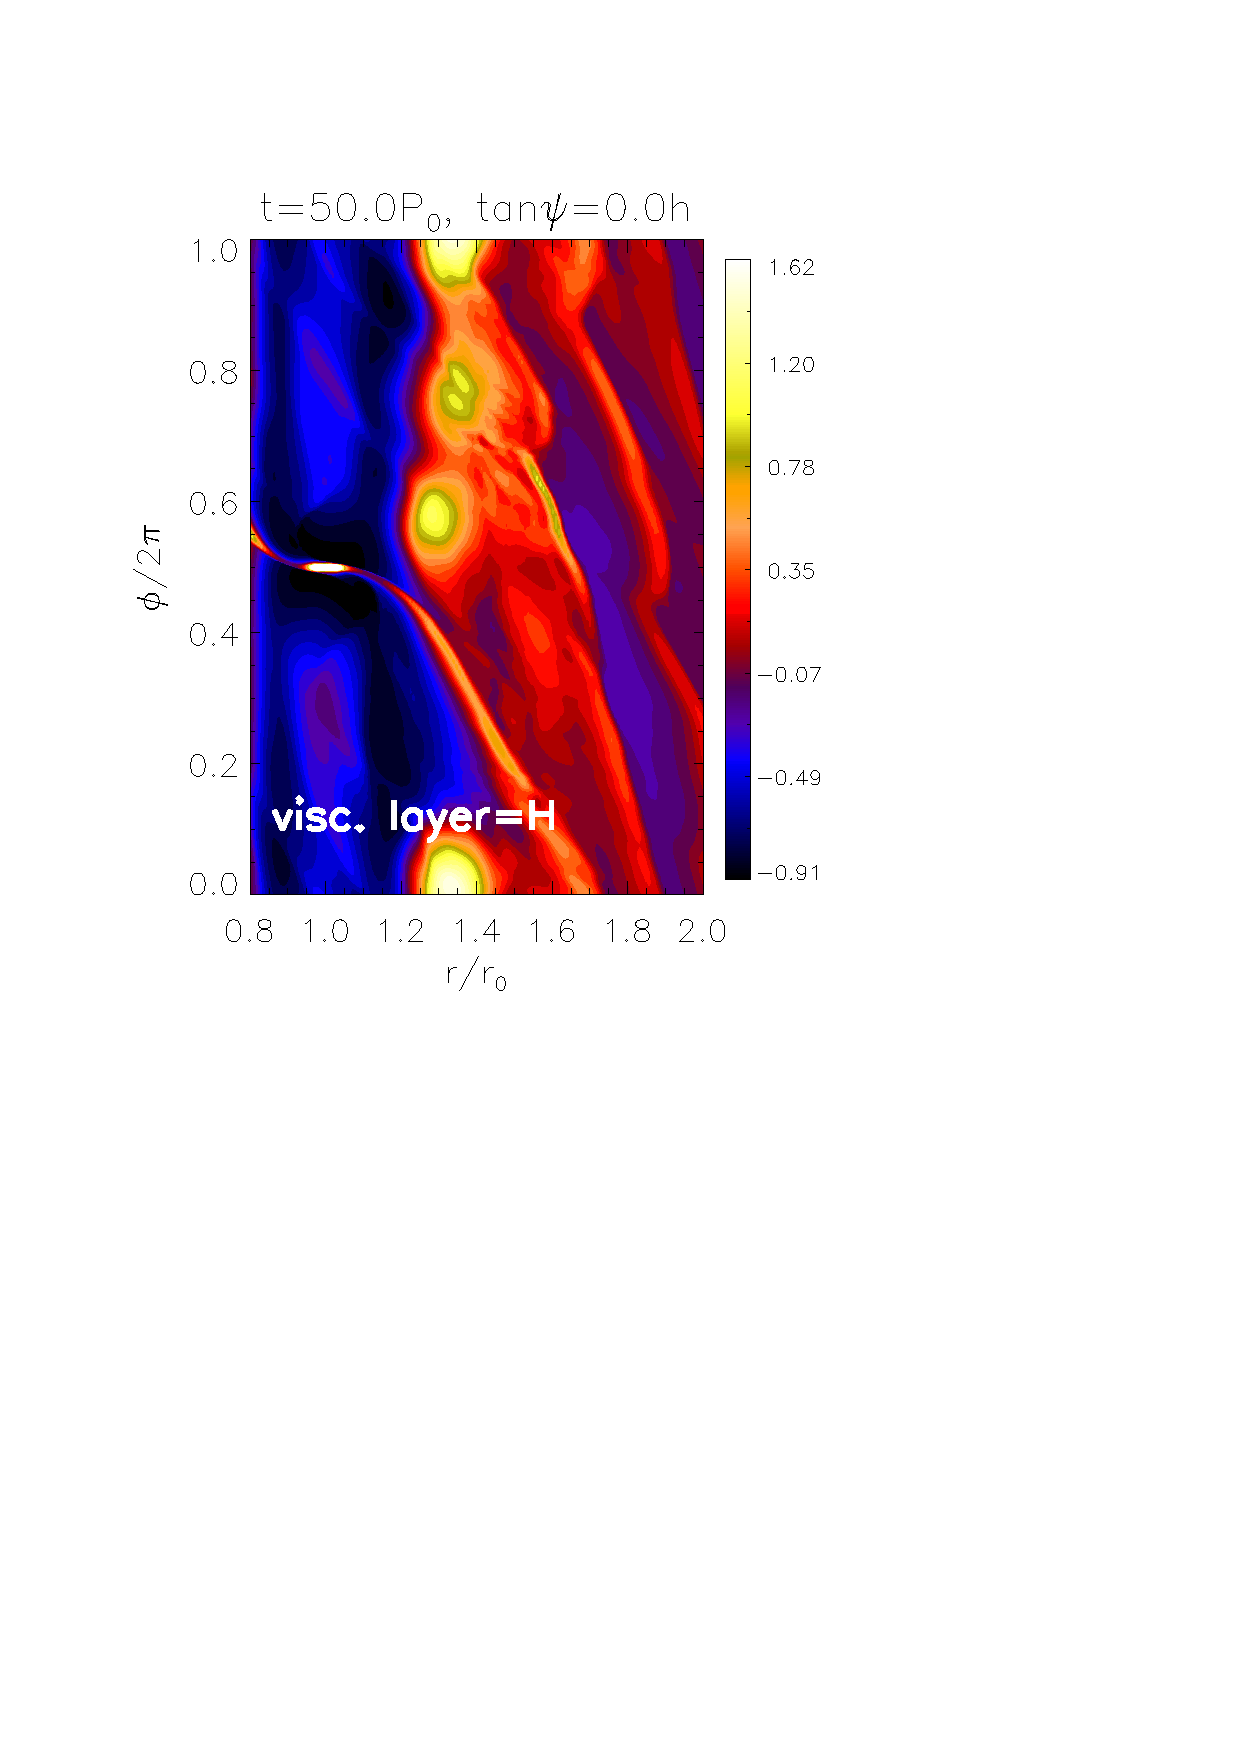
\includegraphics[scale=.43,clip=true,trim=0cm 0.cm 0.cm
    0.9cm]{figures/jup1_3h_pdisk_005}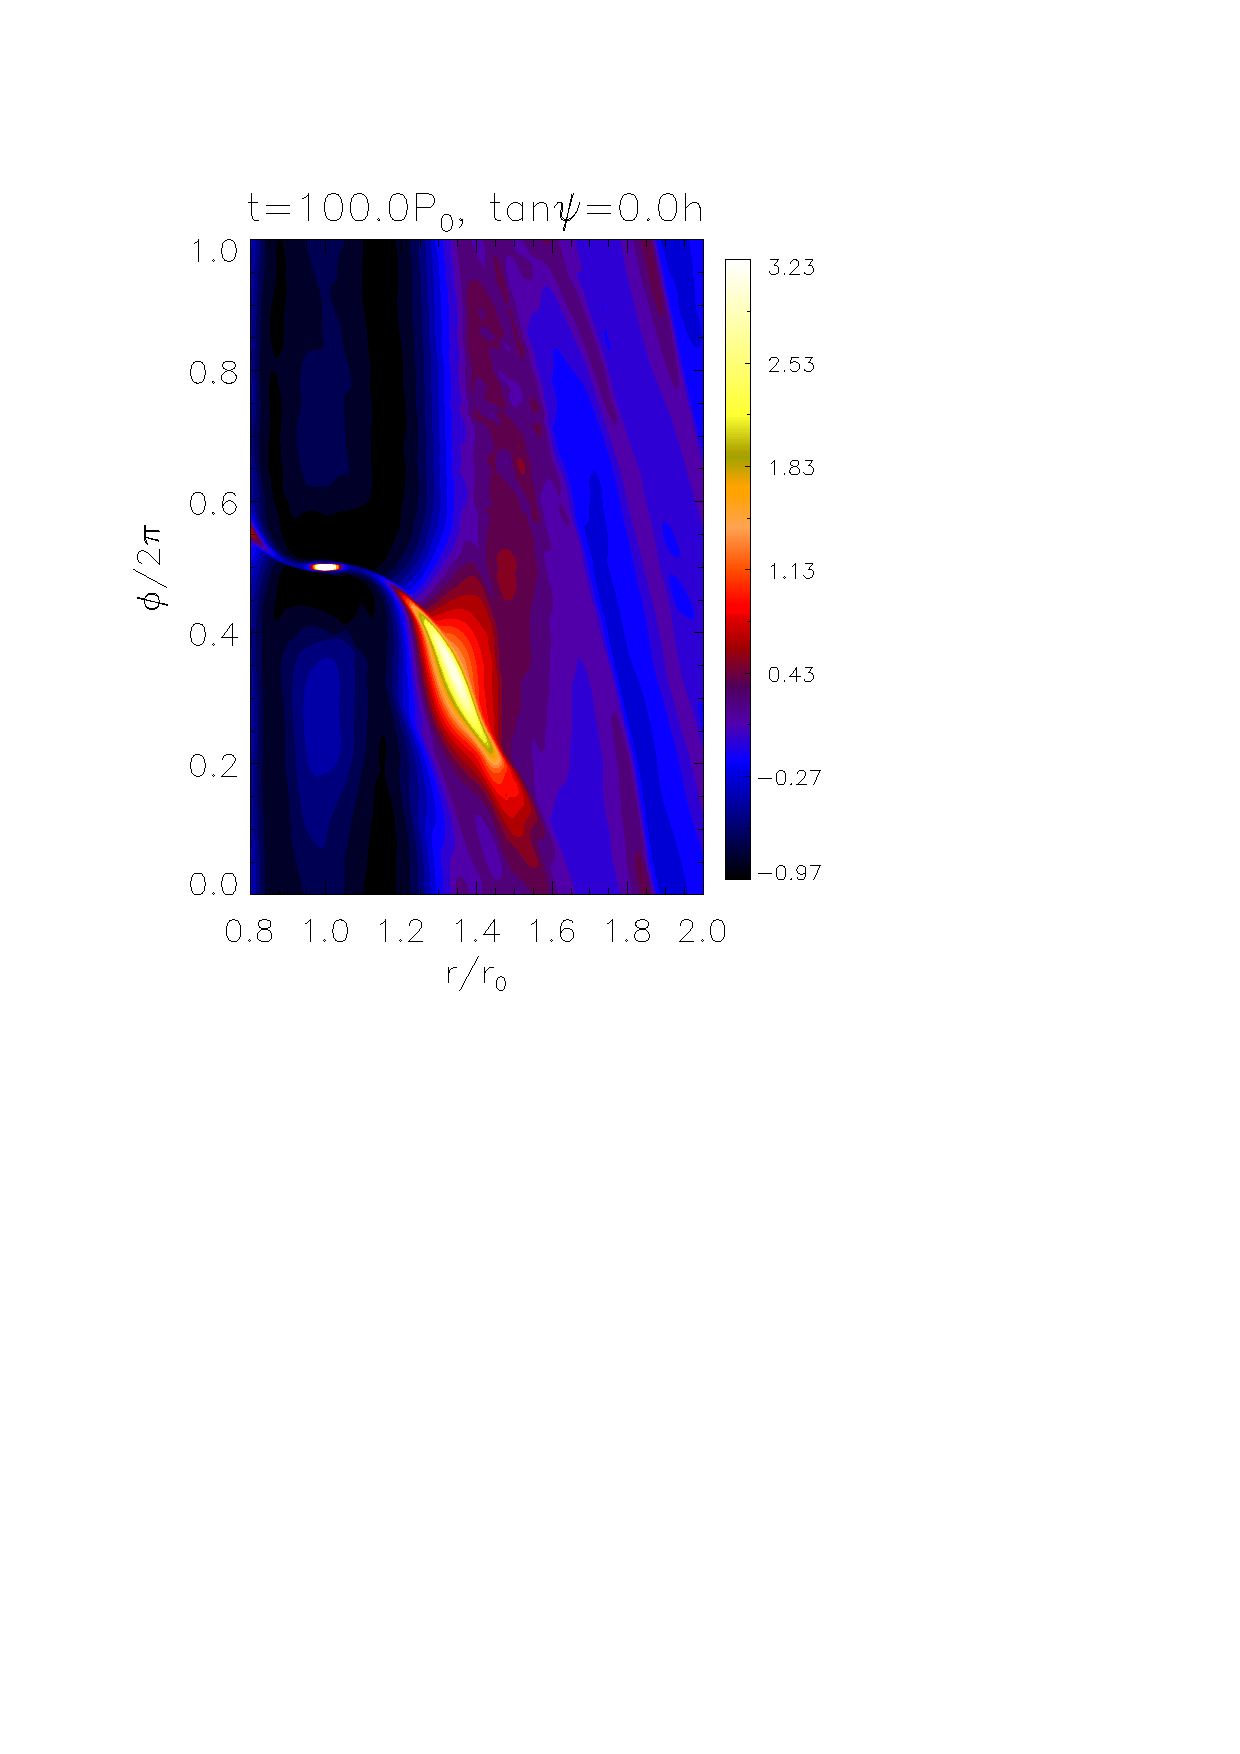
\includegraphics[scale=.43,clip=true,trim=2.3cm
    0.cm 0cm 0.9cm]{figures/jup1_3h_pdisk_010}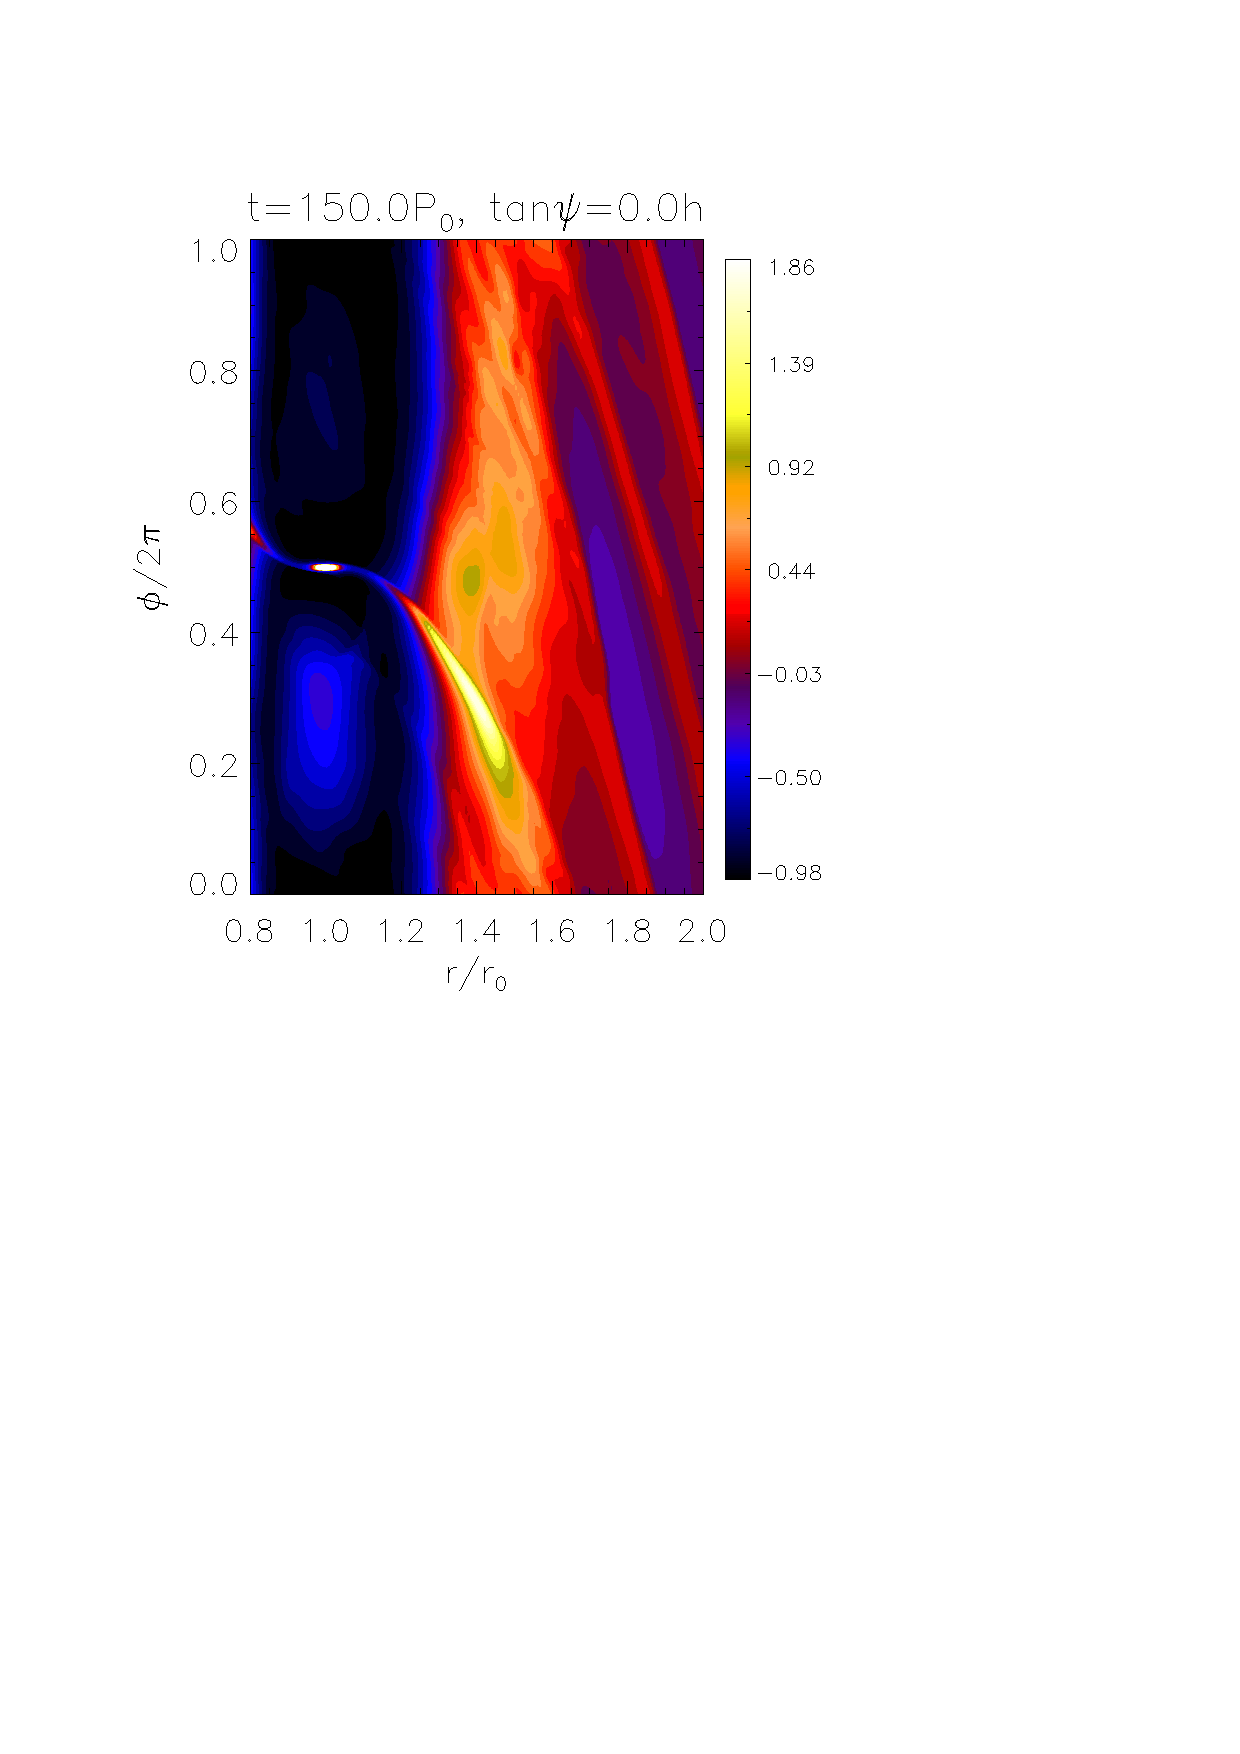
\includegraphics[scale=.43,clip=true,trim=2.3cm
    0.cm 0cm 0.9cm]{figures/jup1_3h_pdisk_015}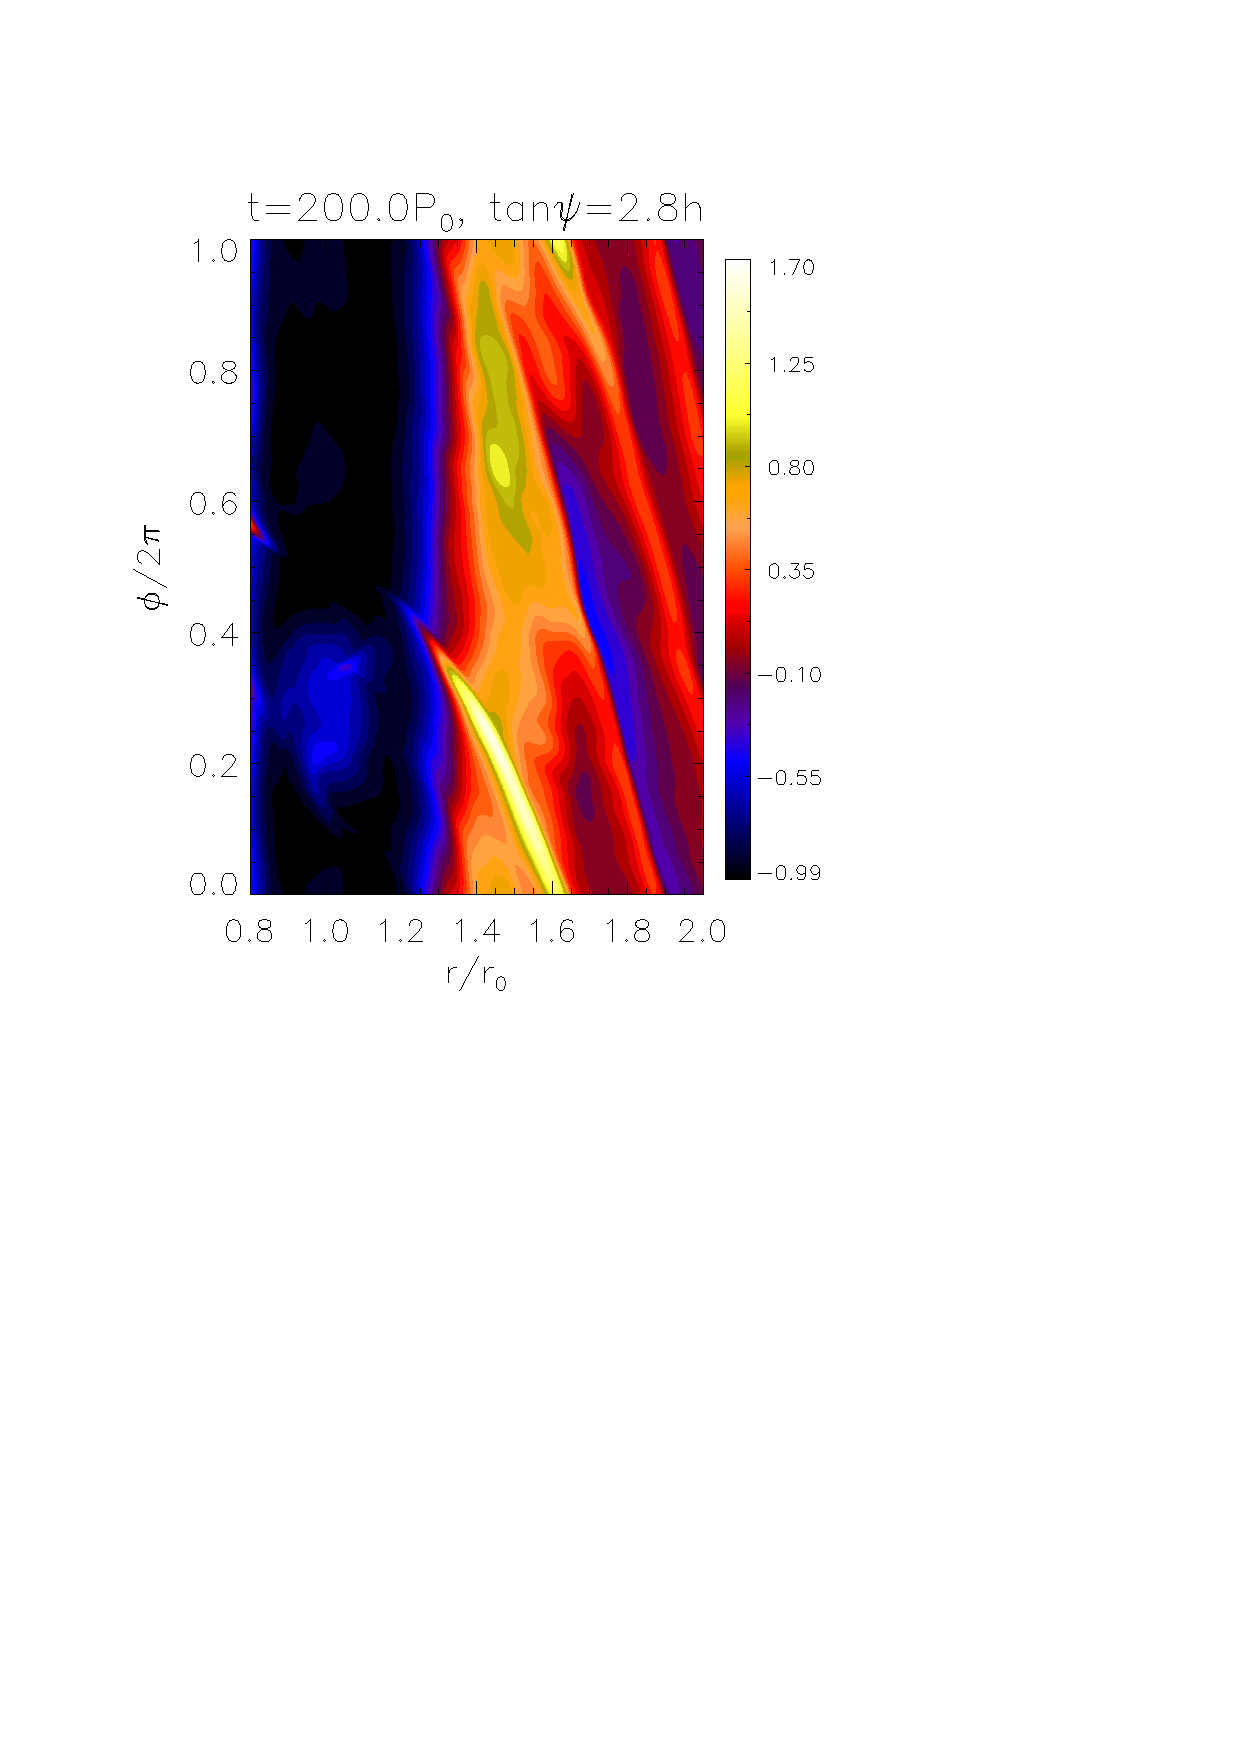
\includegraphics[scale=.43,clip=true,trim=2.3cm
    0.cm 0cm 0.9cm]{figures/jup1_3h_pdisk_020}\\
  %    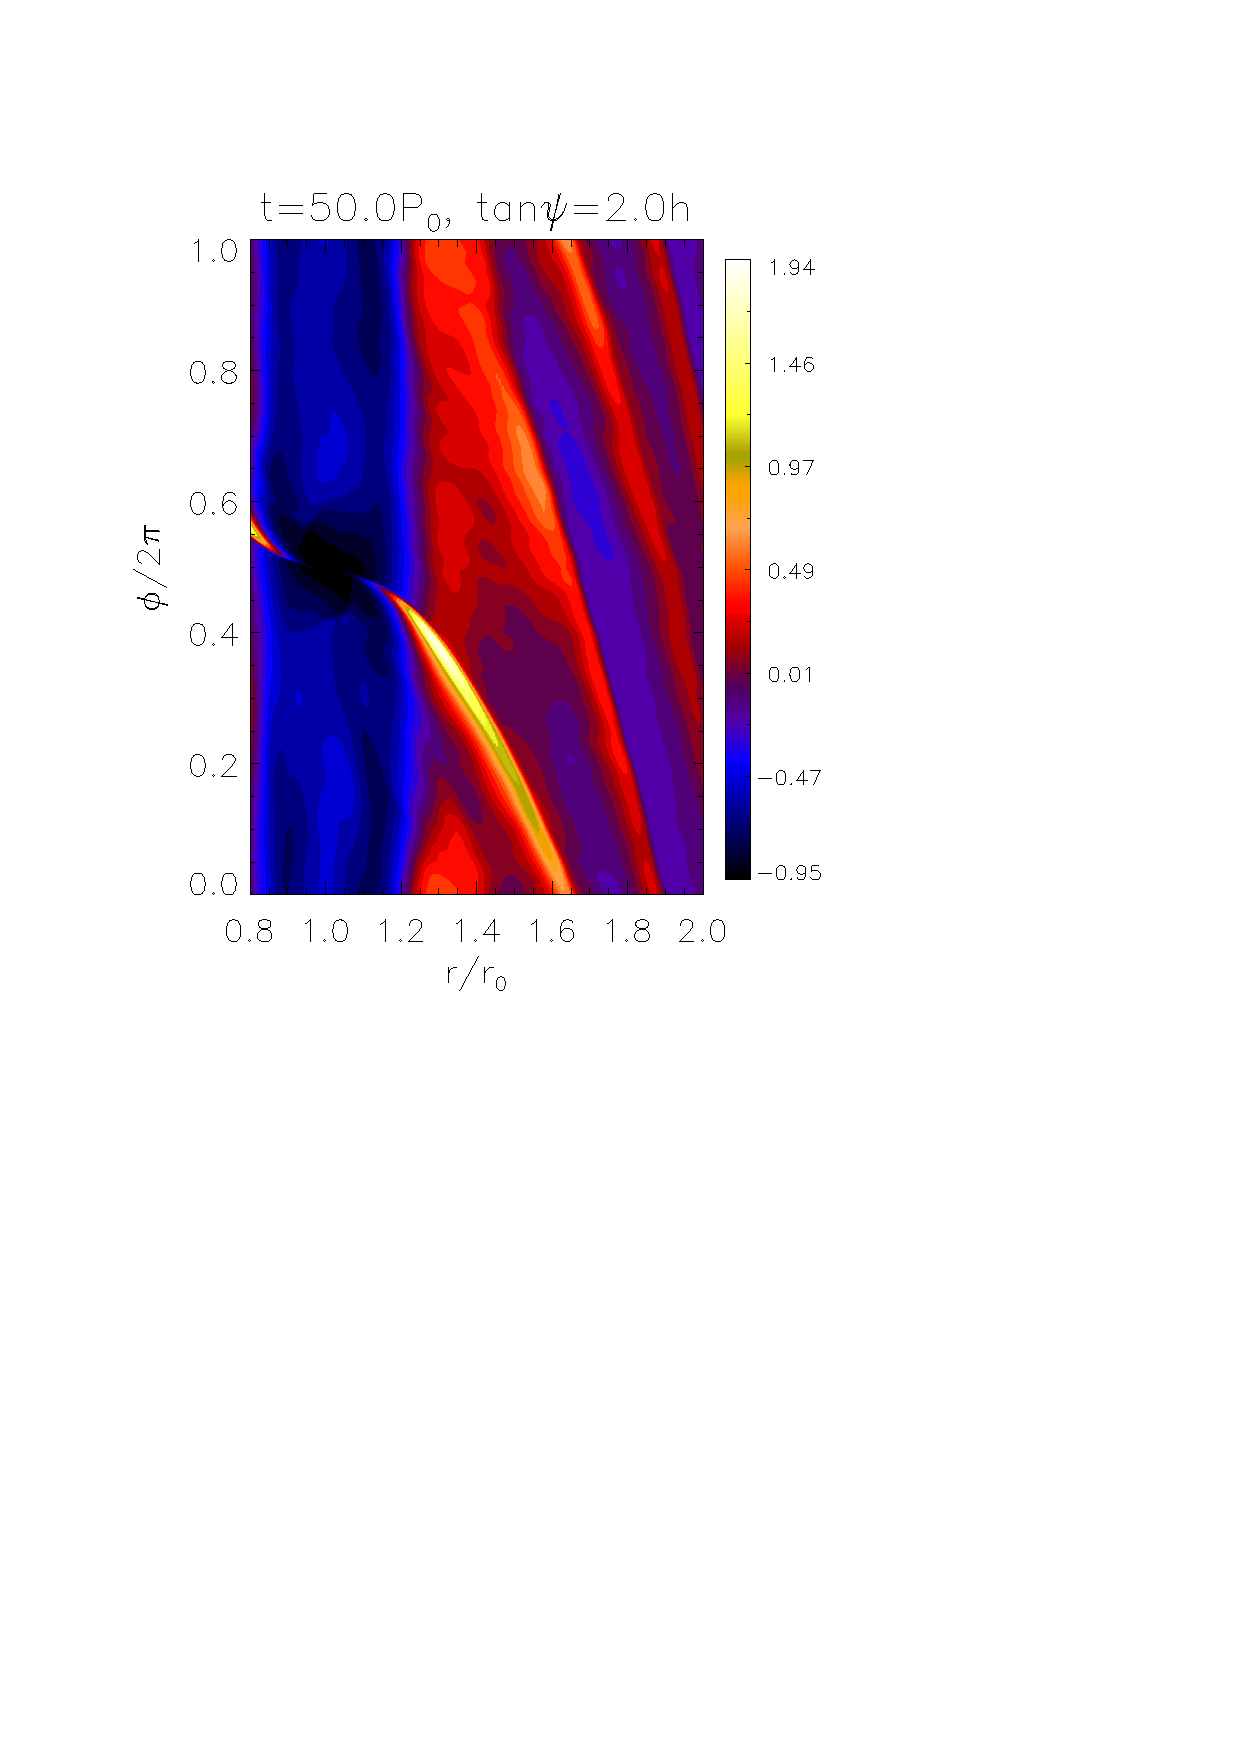
\includegraphics[scale=.43,clip=true,trim=0cm 0.cm 0.cm
  %     0.9cm]{figures/jup2_3h_pdisk_005}
  \caption{Relative density perturbation $\delta\rho$ for disc-planet
    simluations. Top: case P0 (no viscous layer). Bottom: case P1 (viscous layer of $H$). The
    vertical extent of the computational domain is $3H$ and the
    viscous layer is measured from the upper disc boundary.  
    \label{jup0_3h}}
\end{figure*}

\subsubsection{Kinetic energy density}%prob replace with nu_floor=1d-6,
                                %amp=10 sims
Here, we compare the $m=1$ component of the kinetic energy density
($W_1$)  between the no-layer case P0, layered
case P1 and case P0R which is case P0 resumed from $t=100P_0$ with a
viscous layer. Fig. \ref{pdisk_kerz_cases_planet} shows 
$W_1(t)$ averaged over the outer gap edge. For each case we
average $W_1$ over the disc bulk and the atmosphere, and plot them
separately in the figure. 

The $m=1$ component does not emerge from the linear instability, but is a
result of non-linear vortex merging. 
Fig. \ref{pdisk_kerz_cases_planet} shows that merging is accelerated
by a viscous layer: the single vortex appears at $t\sim70P_0$ for case
P1 but only forms at $t\sim120P_0$ for case P0. Also note for all
cases, $W_1$ in the disc bulk (thick lines) is similar to that in the
disc atmosphere (thin lines), implying the $m=1$ disturbance
(i.e. the vortex) evolves two-dimensionally. We checked that this is
consistent with the Froude number $Fr\equiv|Ro|H/z < 1 $ away from the
midplane \citep{barranco05,oishi09}. 

%check froud number is
%less than 1

Case P0R shows that introducing a viscous layer eventually destroys
the vortex. The local viscous timescale $t_\nu\equiv
H^2/\nu\gtrsim 16P_0$ so on short timescales after introducing the 
viscous layer ($t=100P_0$), vortex-merging proceeds in case P0R
similarly to case P0 ($t\in[100,110]P_0$). However, $W_1$ decays for
$t>110P_0$ and evolves towards that of case P1. We expect viscosity
to damp the $m=1$ disturbance in the disc atmosphere between
$t\in[110,200]P_0$ because this corresponds to $\sim 6 t_\nu$, but 
the disturbance in the disc bulk is also damped out: the evolution
remains two-dimensional.    

\begin{figure}
  \centering
  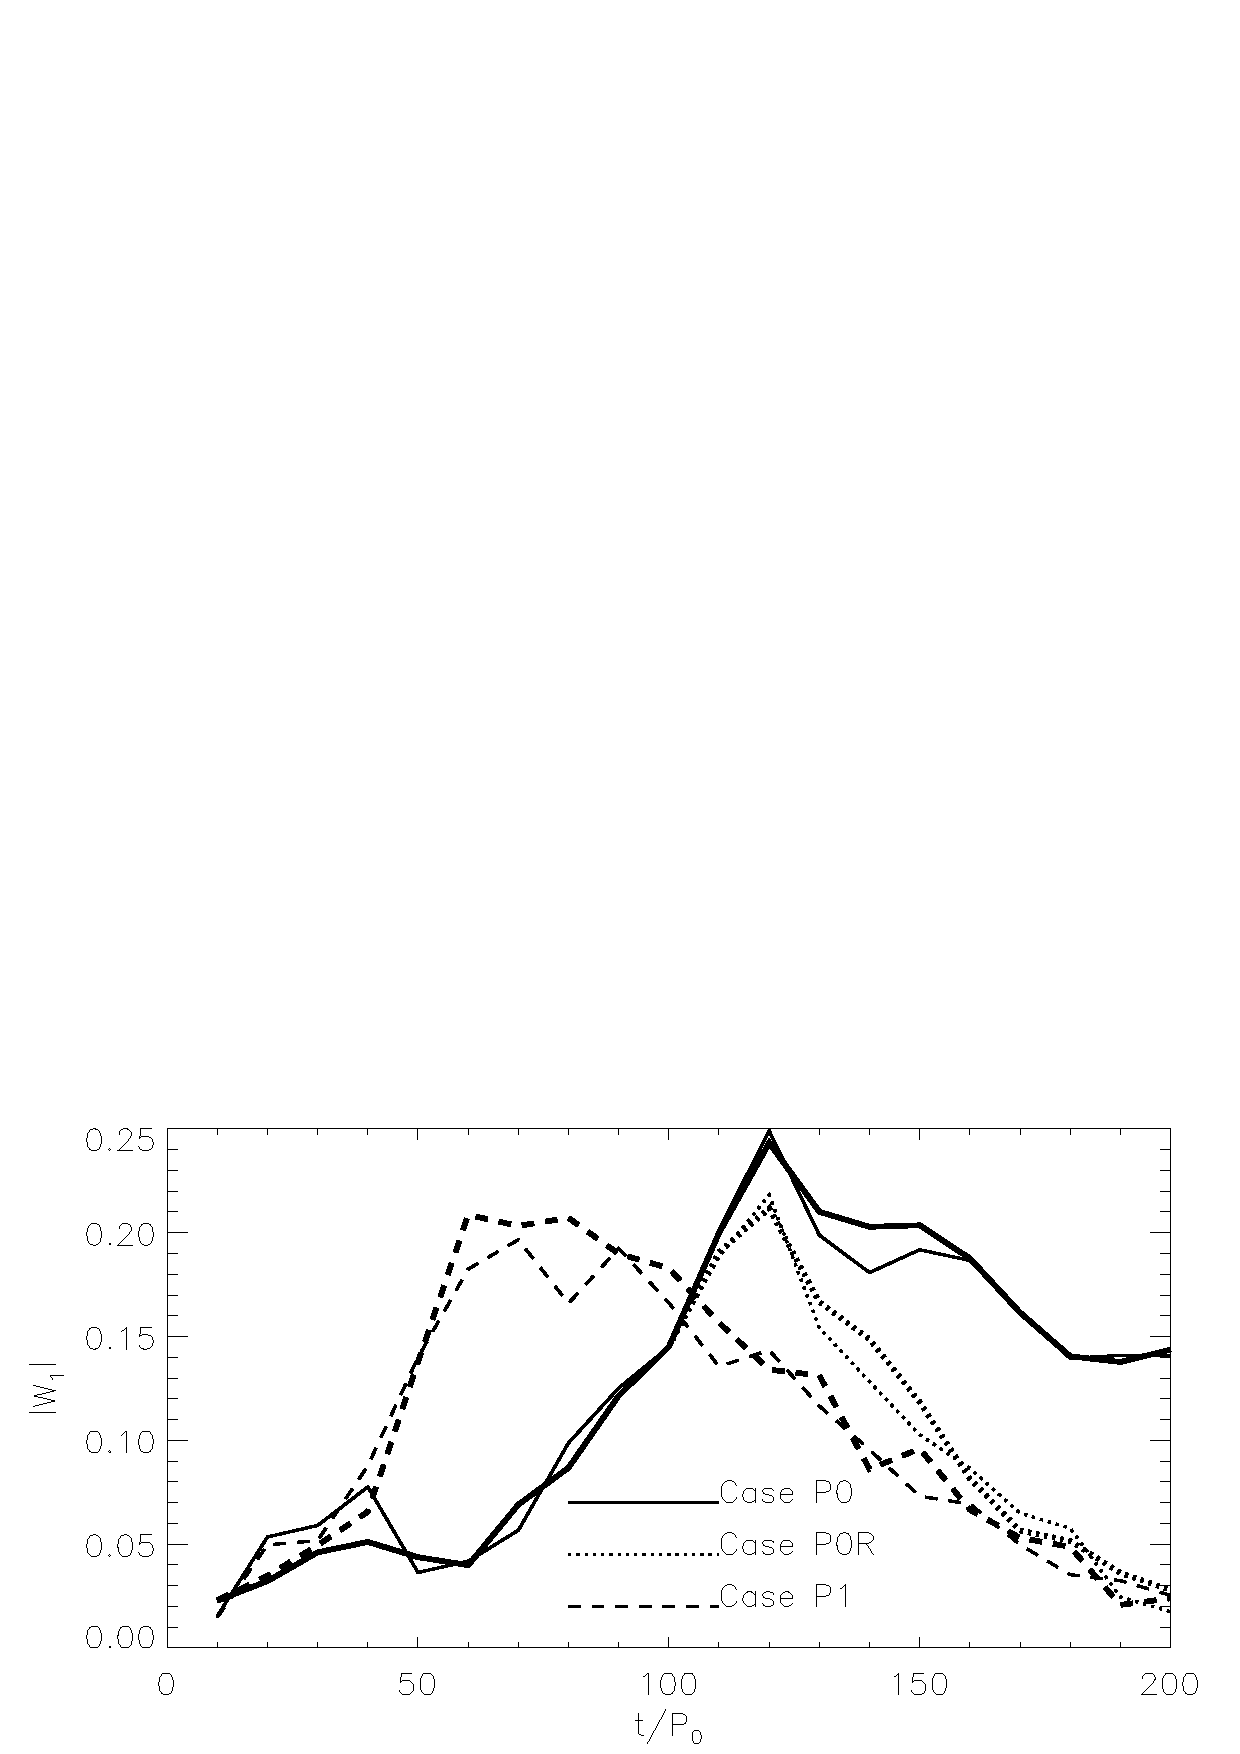
\includegraphics[width=\linewidth]{figures/pdisk_kerz_cases_planet_m1}
  \caption{Evolution of the $m=1$ component of kinetic energy density,
    averaged over $r\in[1.2,1.6]r_0$. This average
    is split into that taken over disc bulk ($z\in[0,2]H$, thick
    lines) and the disc atmosphere ($z\in[2,3]H$, thin lines). Case P0
    has no viscous layer (solid) and case P1 has a viscous layer in
    $z\in[2,3]H$ (dashed). Case P0R is identical to case P0 up to $t=100P_0$,
    but was simulated with a viscous layer of thickness
    $H$ for $t>100P_0$. 
\label{pdisk_kerz_cases_planet}}
\end{figure}

We emphasize the kinetic energy is dominated by horizontal
motions, with $\mathrm{max}(|v_z|/|\bm{v}|) < 0.03$ at the outer
gap edge ($r\in[1.2,1.6]r_0$). Vertical motions are well sub-sonic. When averaged
over $z\in[0,2]H$ and $z\in[2,3]H$, the vertical Mach number
$M_z\equiv|v_z|/c_s=0.05,\,0.08$ (P0), $M_z=0.04,\,0.05$ (P0R) and
$M_z=0.05,0.06$ (P1), respectively. That is, $|v_z|$
increases with height, but the difference between $v_z$ in the disc
atmosphere and that near the midplane diminishes when viscosity is
present in the former. 

\subsubsection{Potential vorticity}
We examine the PV evolution for case P0R in
Fig. \ref{jup0_3h_visc_restart_vorten}, but  
to higlight the vortices, which are positive (negative)
density (vertical vorticity) perturbations, we show the inverse PV
perturbation, $\eta_z(t=0)/\eta_z - 1$. As noted above, a single vortex still forms
despite introducing a viscous layer at $t=100P_0$. However, this
vortex decays rapidly compared to case P0. The vortex elongates, 
producing a `tail' ($t=160P_0$), and eventually the vortex core
disappears altogether.  


\begin{figure*}
  \centering
  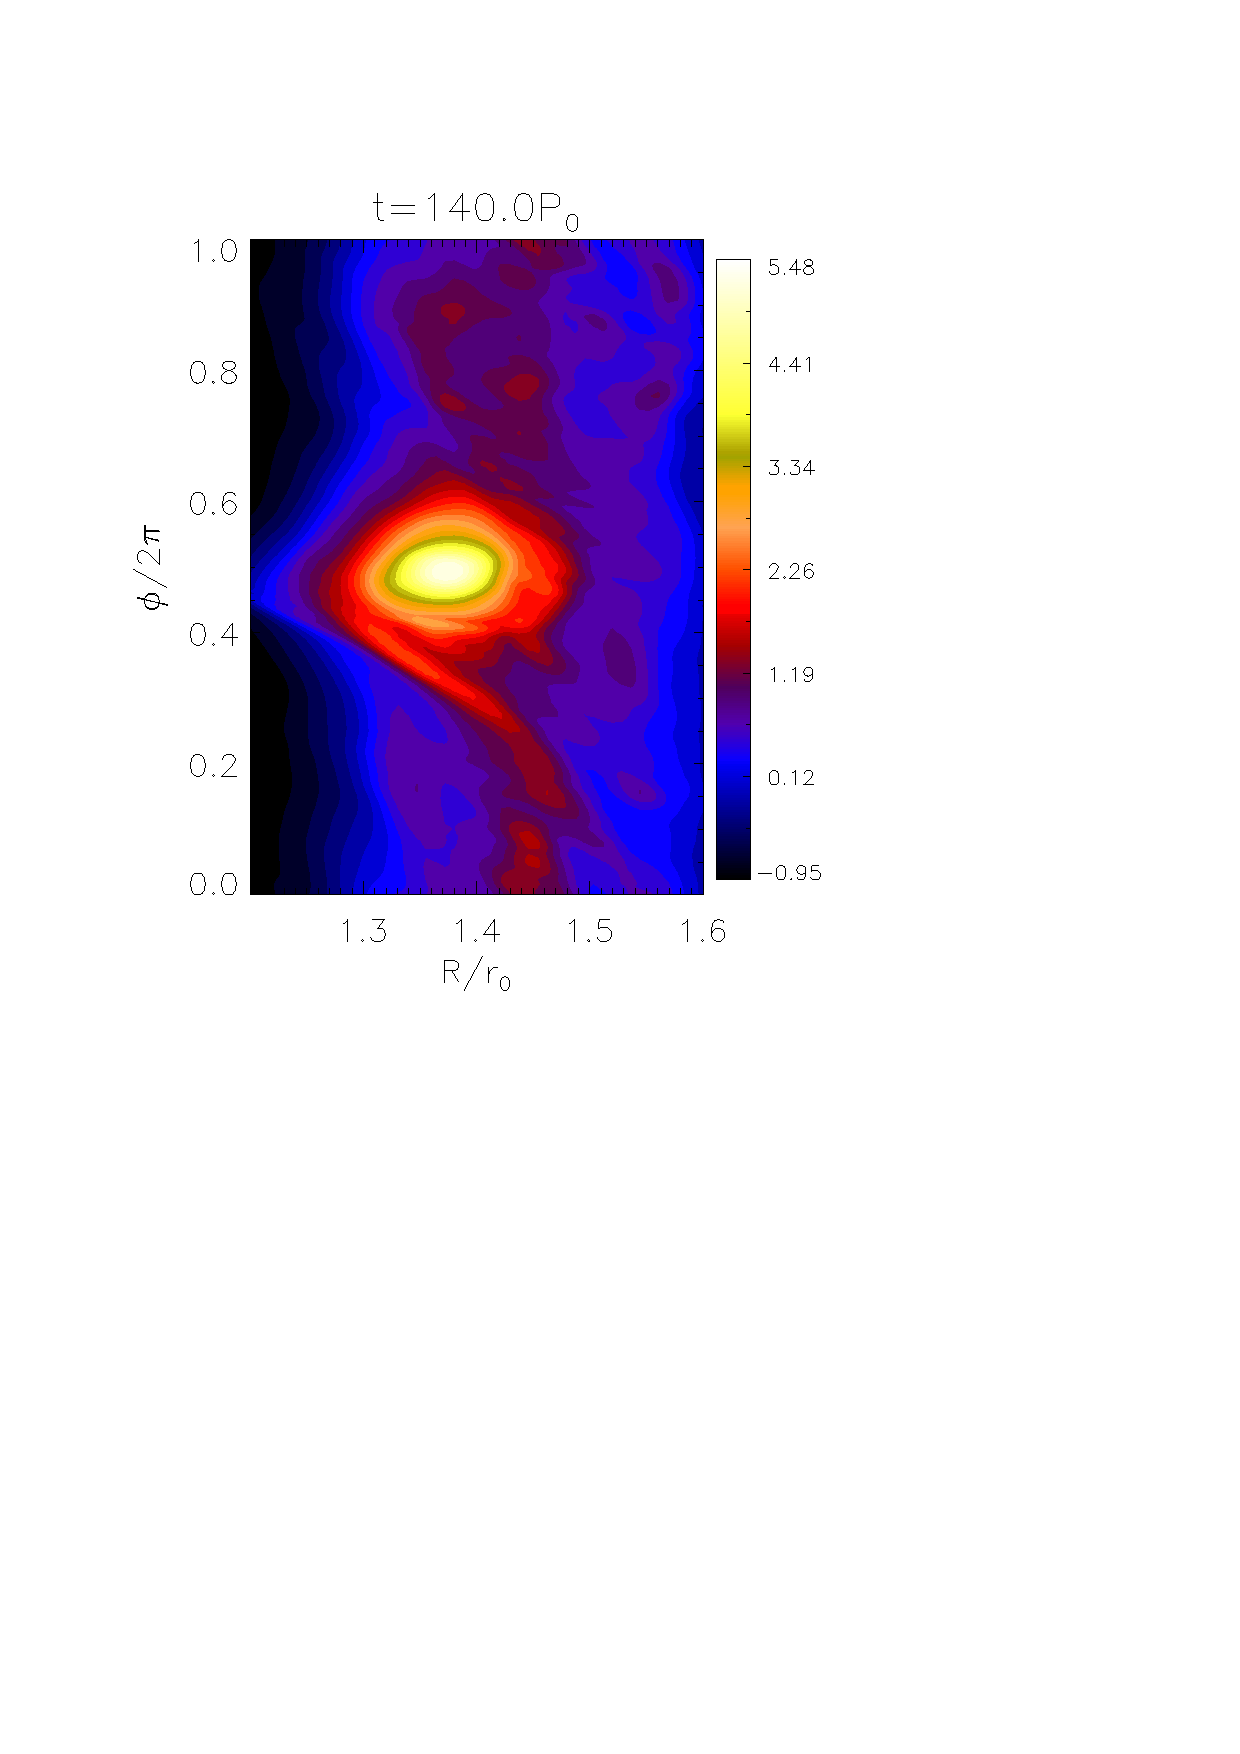
\includegraphics[scale=.43,clip=true,trim=0cm .0cm 0cm
    0cm]{figures/jup0_3h_visc_restart_pdisk_vorten_014}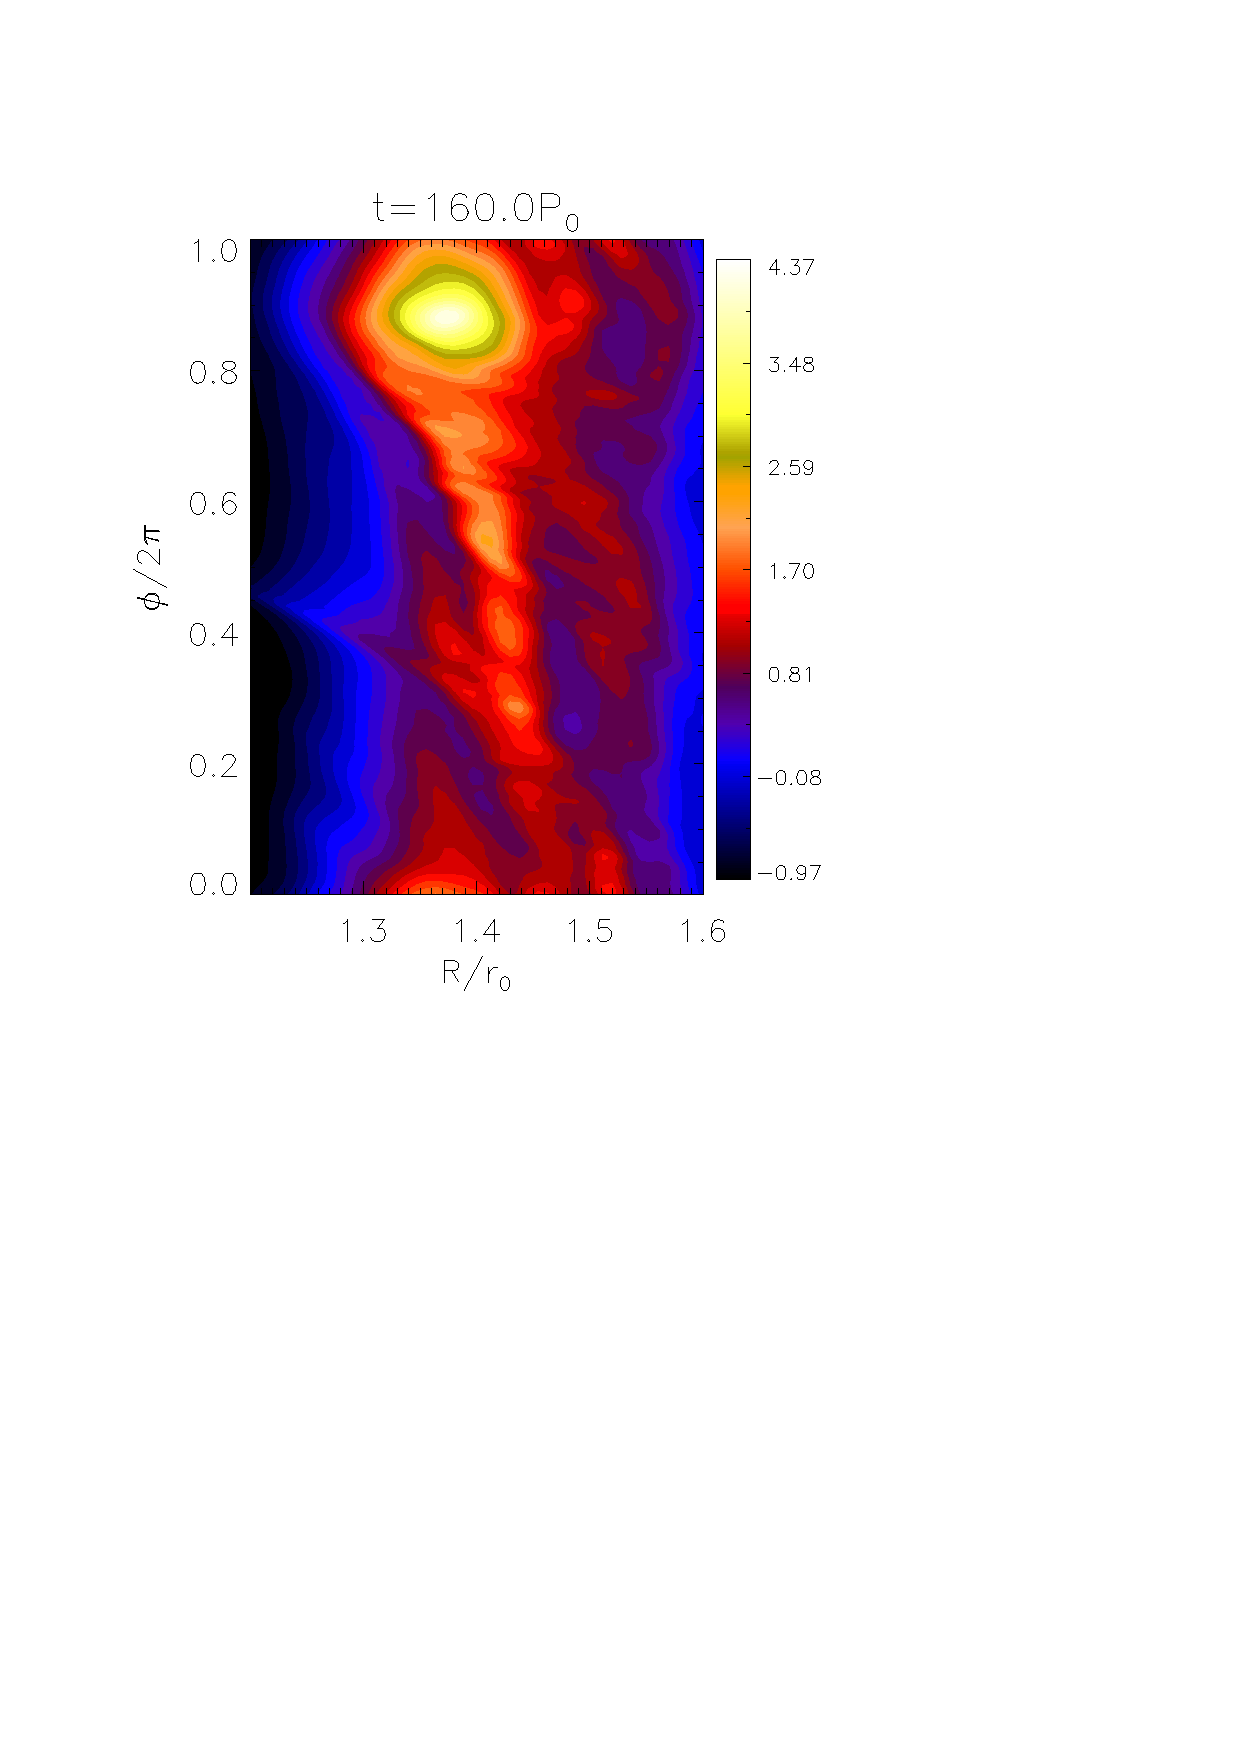
\includegraphics[scale=.43,clip=true,trim=2.3cm
    .0cm 0cm 0cm]{figures/jup0_3h_visc_restart_pdisk_vorten_016}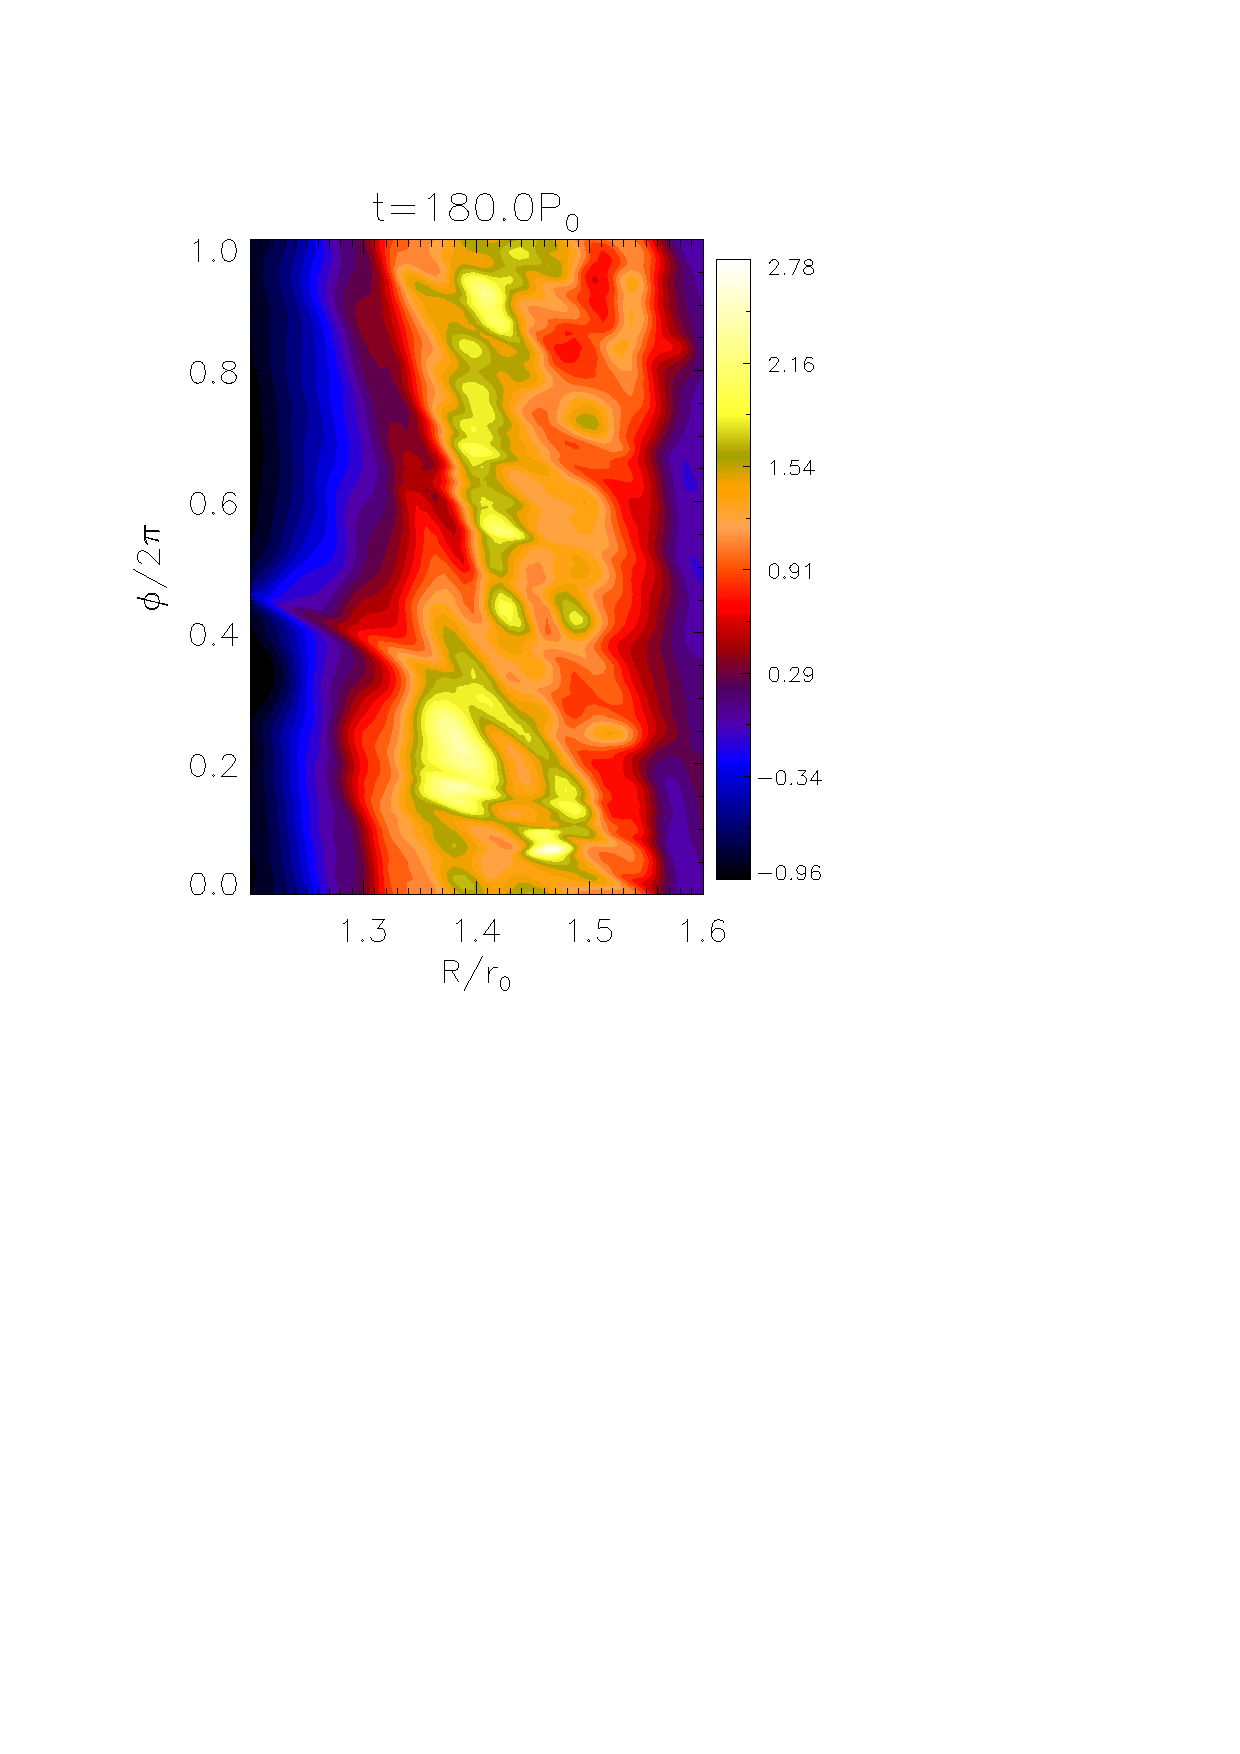
\includegraphics[scale=.43,clip=true,trim=2.3cm
    .0cm 0cm 0cm]{figures/jup0_3h_visc_restart_pdisk_vorten_018}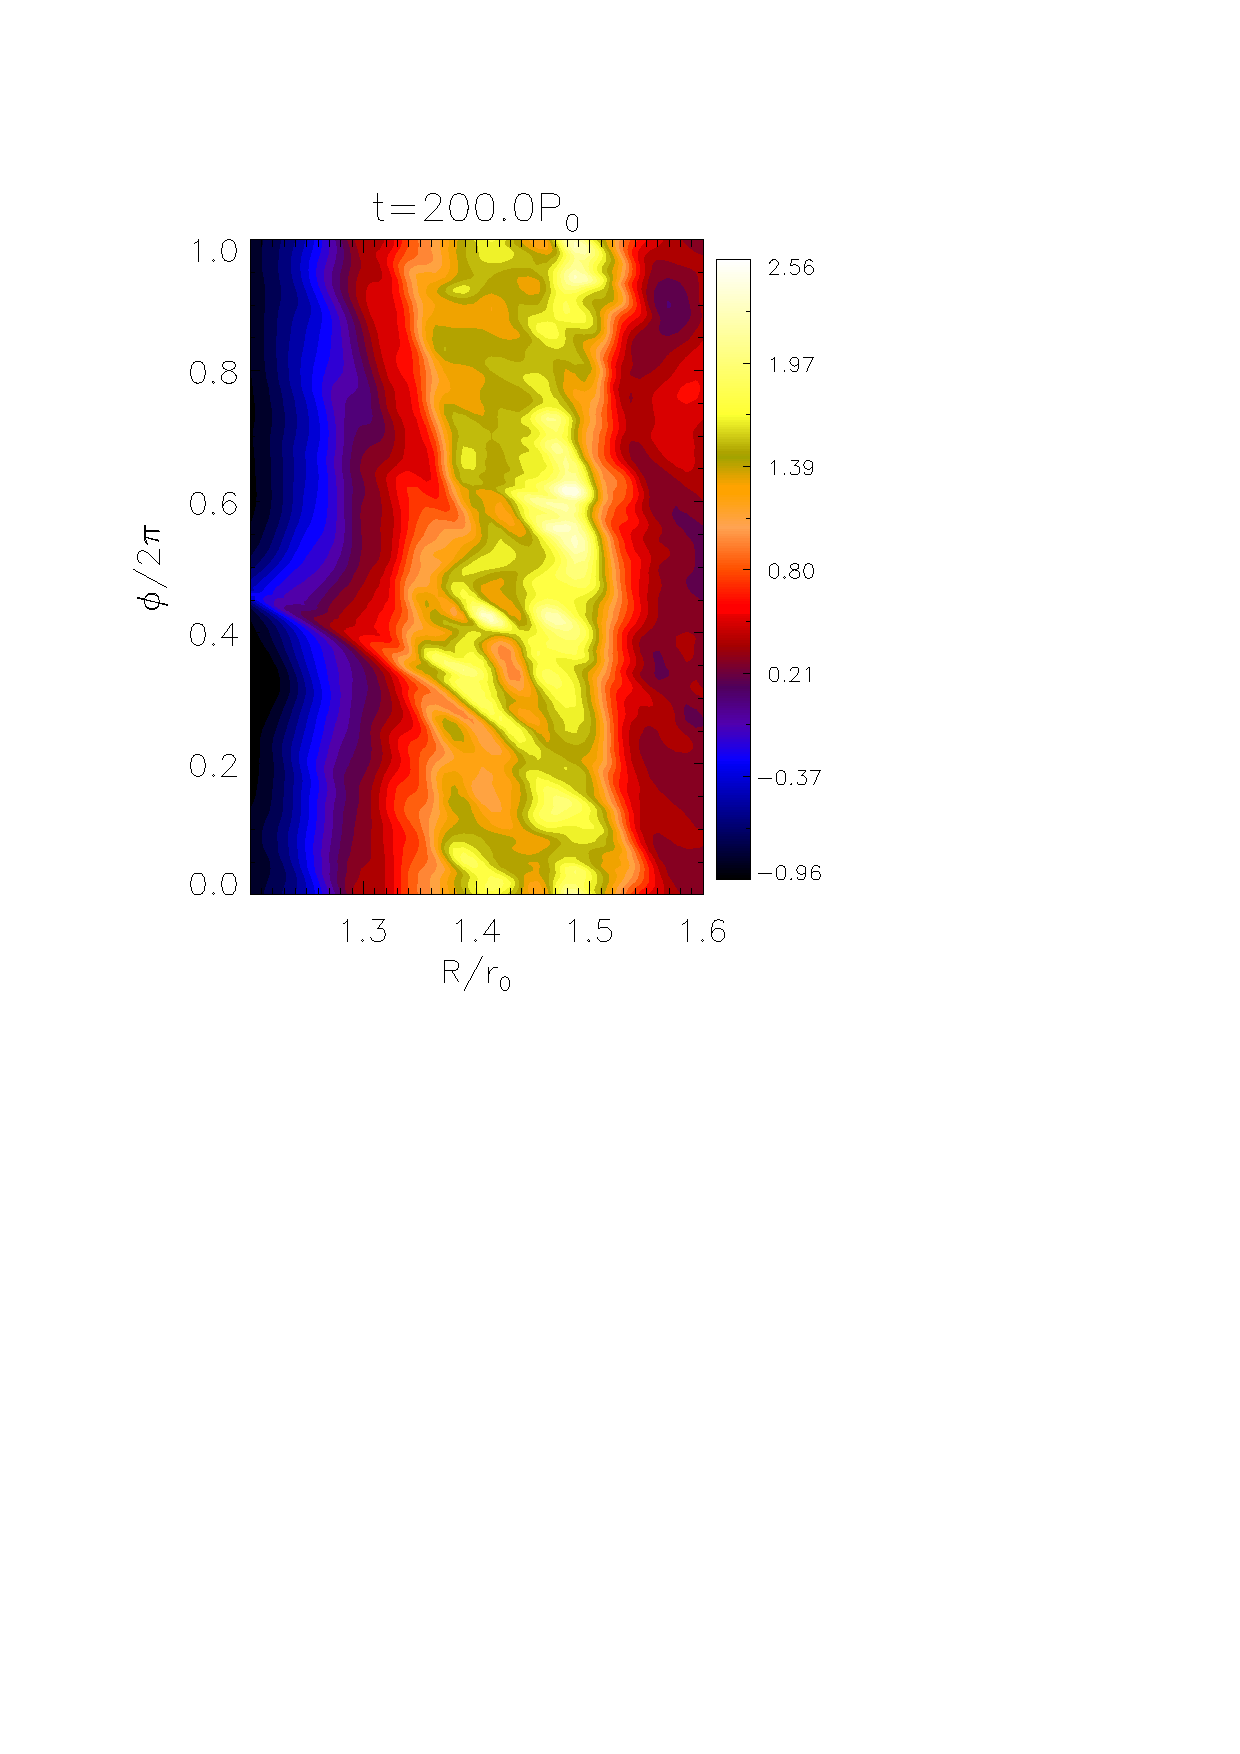
\includegraphics[scale=.43,clip=true,trim=2.3cm
    .0cm 0cm 0cm]{figures/jup0_3h_visc_restart_pdisk_vorten_020}
  \caption{Inverse PV perturbation for case P0R, which was resumed
    from the no-layer case P0 from $t=100P_0$ with the introduction of
    a viscous layer of $H$. 
    \label{jup0_3h_visc_restart_vorten}}
\end{figure*}

\subsubsection{Resolution check}%prob just commentary
We repeated simulations P0 and P1 with resolution
$(N_r,N_\theta,N_\phi)=(512,96,1536)$, corresponding
to $12$ and $32$ cells per scale-height in $(r,\phi)$ and $\theta$,
respectively. We denote these runs as P0HR and P1HR below. 

We observe similar evolution in P0HR and P1HR as their standard
resolution versions. However, due to lower numerical diffusion, we
find stronger vortices in P0HR. Although the vortex in P1HR persisted
longer than the standard resolution run, it was still subject to rapid
%%how long? 
decay in comparison with P0HR. At the end of the simulation we find
the $m=1$ amplitude to be $a_1=0.29$ and $a_1=0.10$, respectively for
P0HR and P1HR; a similar contrast as that bewteen P0 and P1.    

%Interestingly, we observe small-scale instability inside the
%vortex. This is shown in Fig. . We suspect this is the elliptic
%instability, but cannot prove this. It is absent in P1HR.  

\subsection{Additional simulations}% higher visc, strict isothermal 
Locally isothermal, low viscosity discs are vulnerable to the
so-called `vertical shear 
instability' because $\partial_z\Omega_i\neq 0$ \citep{nelson12}. 
\citeauthor{nelson12} employed a radial  resolution $\gtrsim 60$ cells
per $H$ to resolve this instability because it involves small radial
wavelengths ($\ll H$). Our numerical resolution is unlikely to capture
this instability. Nevertheless, we have performed additional
simulations designed to eliminate the vertical shear instability.   

\subsubsection{Larger floor viscosity}
We performed several simulations with $\hat{\nu}_0=10^{-6}$. A viscosity of
$\hat{\nu}\sim 10^{-6}$ is expectd to damp the vertial shear 
instability \citep{nelson12}, while still permitting the gap-edge
RWI. Table \ref{planet_sims} summarises
these cases with $A_\nu=10$ (`Pb' runs) and $A_\nu=100$ (`Pc' runs). 

In these simulations we find vortices eventually decay, even in the
no-layer case Pb0. For $A_\nu=10$, the layered cases Pb0.5 and Pb1 evolve
similarly Pb0: three vortices formed by $t\sim30P_0$, merging into two
vortices by $t\sim40P_0$, then finally into a single vortex by
$t\sim130P_0$, which subsequently decays. However, the final vortex
decays faster in the presence of a viscous layer. This is shown in
Fig. \ref{pdisk_kerz_cases_planet_hivisc}, which compares the $m=1$
kinetic energy density for case Pb0 and Pb1. The evolution only begins
to differ after the single-vortex has formed. 

\begin{figure}
  \centering
  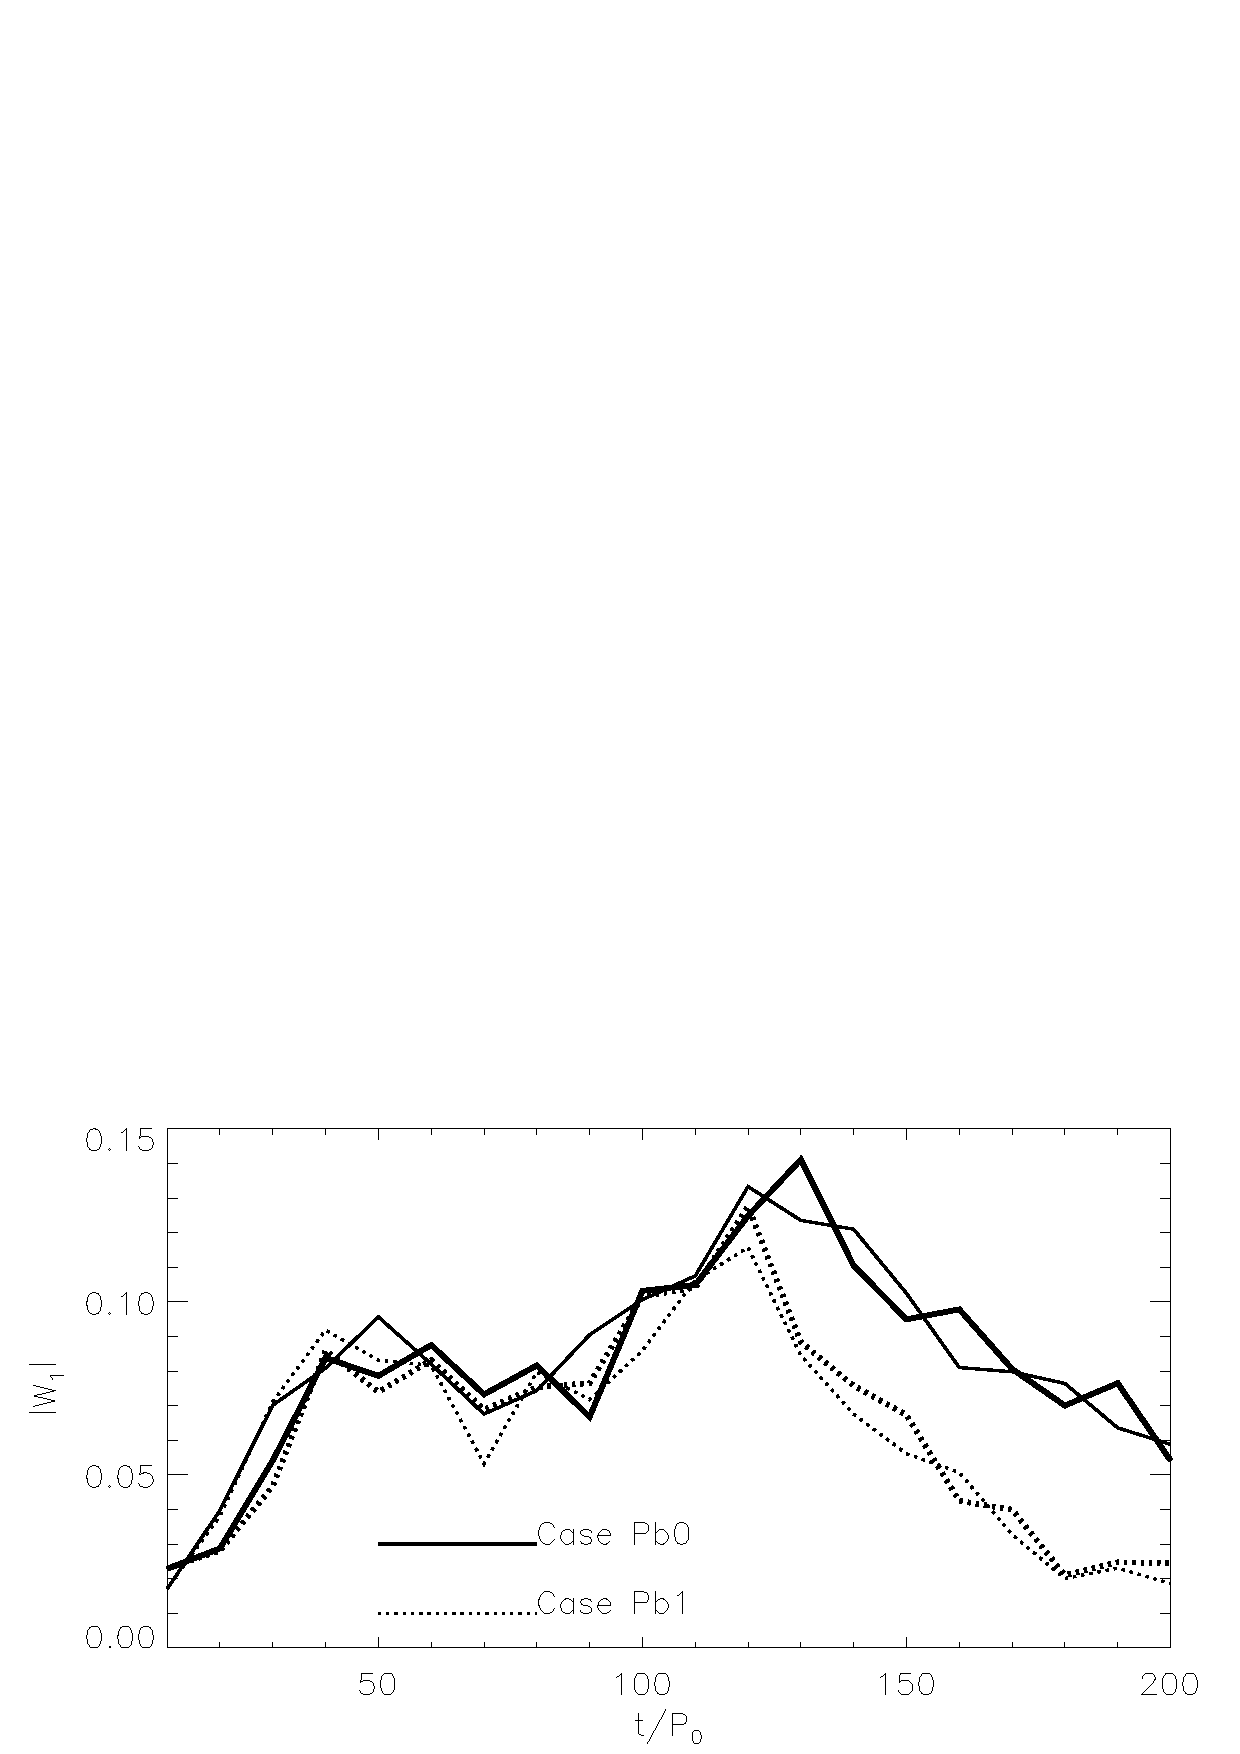
\includegraphics[width=\linewidth]{figures/pdisk_kerz_cases_nu6}
  \caption{Same as Fig. \ref{pdisk_kerz_cases_planet} but with
    floor viscosity $\hat{\nu}_0=10^{-6}$: cases Pb0 (solid, no viscous layer) and Pb1
    (dotted, viscous layer of $H$). The thick (thin) lines indicate
    $W_1$ averaged over $z\in[0,2]H$
    ($z\in[2,3]H$). 
    \label{pdisk_kerz_cases_planet_hivisc}}
\end{figure}


For $A_\nu=100$ (cases Pc0.5 and Pc1), we find the $m=2$ amplitude
dominated over $m=1$, so a single-vortex configuration never
forms. For both Pc0.5 and Pc1 the $m=2$ (two-vortex configuration)
amplitude decreases from $t\sim 50P_0$. For case Pc1, the vortices are
transient features and are entirely absent for $t\gtrsim80P_0$.  


\subsubsection{Strictly isothermal discs} 
We repeated simulations P0, P1 and Q1 with a strictly isothermal
equation of state ($q=0$). These are summarised in Table
\ref{planet_sims_iso}. Fig. \ref{pdisk_kerz_cases_planet_iso} compares
the $m=1$ kinetic energy density for these cases. Consistent with the
above simulations, a viscous layer causes a faster decay in this
quantity. Most interesting though, is that we found case Iso2 (with a viscous
layer of $\sim H$) only shows very weak non-axisymmetric perturbations
early on ($t\lesssim 50P_0$): vortex formation is surpressed. 


%and the end, vortices in all cases?  

\begin{table}
  \centering
  \caption{Disc-planet simulations with a strictly
    isothermal equation of state ($q=0$). The thickness of the viscous layer
    is quoted at the reference radius $R=r_0$. \label{planet_sims_iso}}
    \begin{tabular}{llllrc}
      \hline\hline
      Case & $10^6\hat{\nu}_0$ & $A_\nu$ & visc. layer& $10^2\overline{a}_1$ &vortex \\ 
      \hline
      Iso0   & 1.0  & 1          & 0      & 19.3  &  YES   \\
      Iso1   & 1.0  & 10         & $H_0$  & 12.8  &  YES     \\ 
      Iso2   & 1.0  & 100        & $H_0$  & 1.1  &  NO     \\ 
      \hline
  \end{tabular}
\end{table}

%Fig. \ref{iso_vorten} shows the inverse PV perturbation for isothermal
%disc-planet simulations. Again, in all cases we observe the RWI to
%grow initially (we identified non-axisymmetric disturbances for
%$t\lesssim 50P_0$). These disturbances merge into a single vortex in the
%no-layer case Iso0. However, case Iso2 does not develop the single vortex in
%the non-linear regime: the gap edge becomes axisymmetric and remains
%stable. 


\begin{figure}
  \centering
  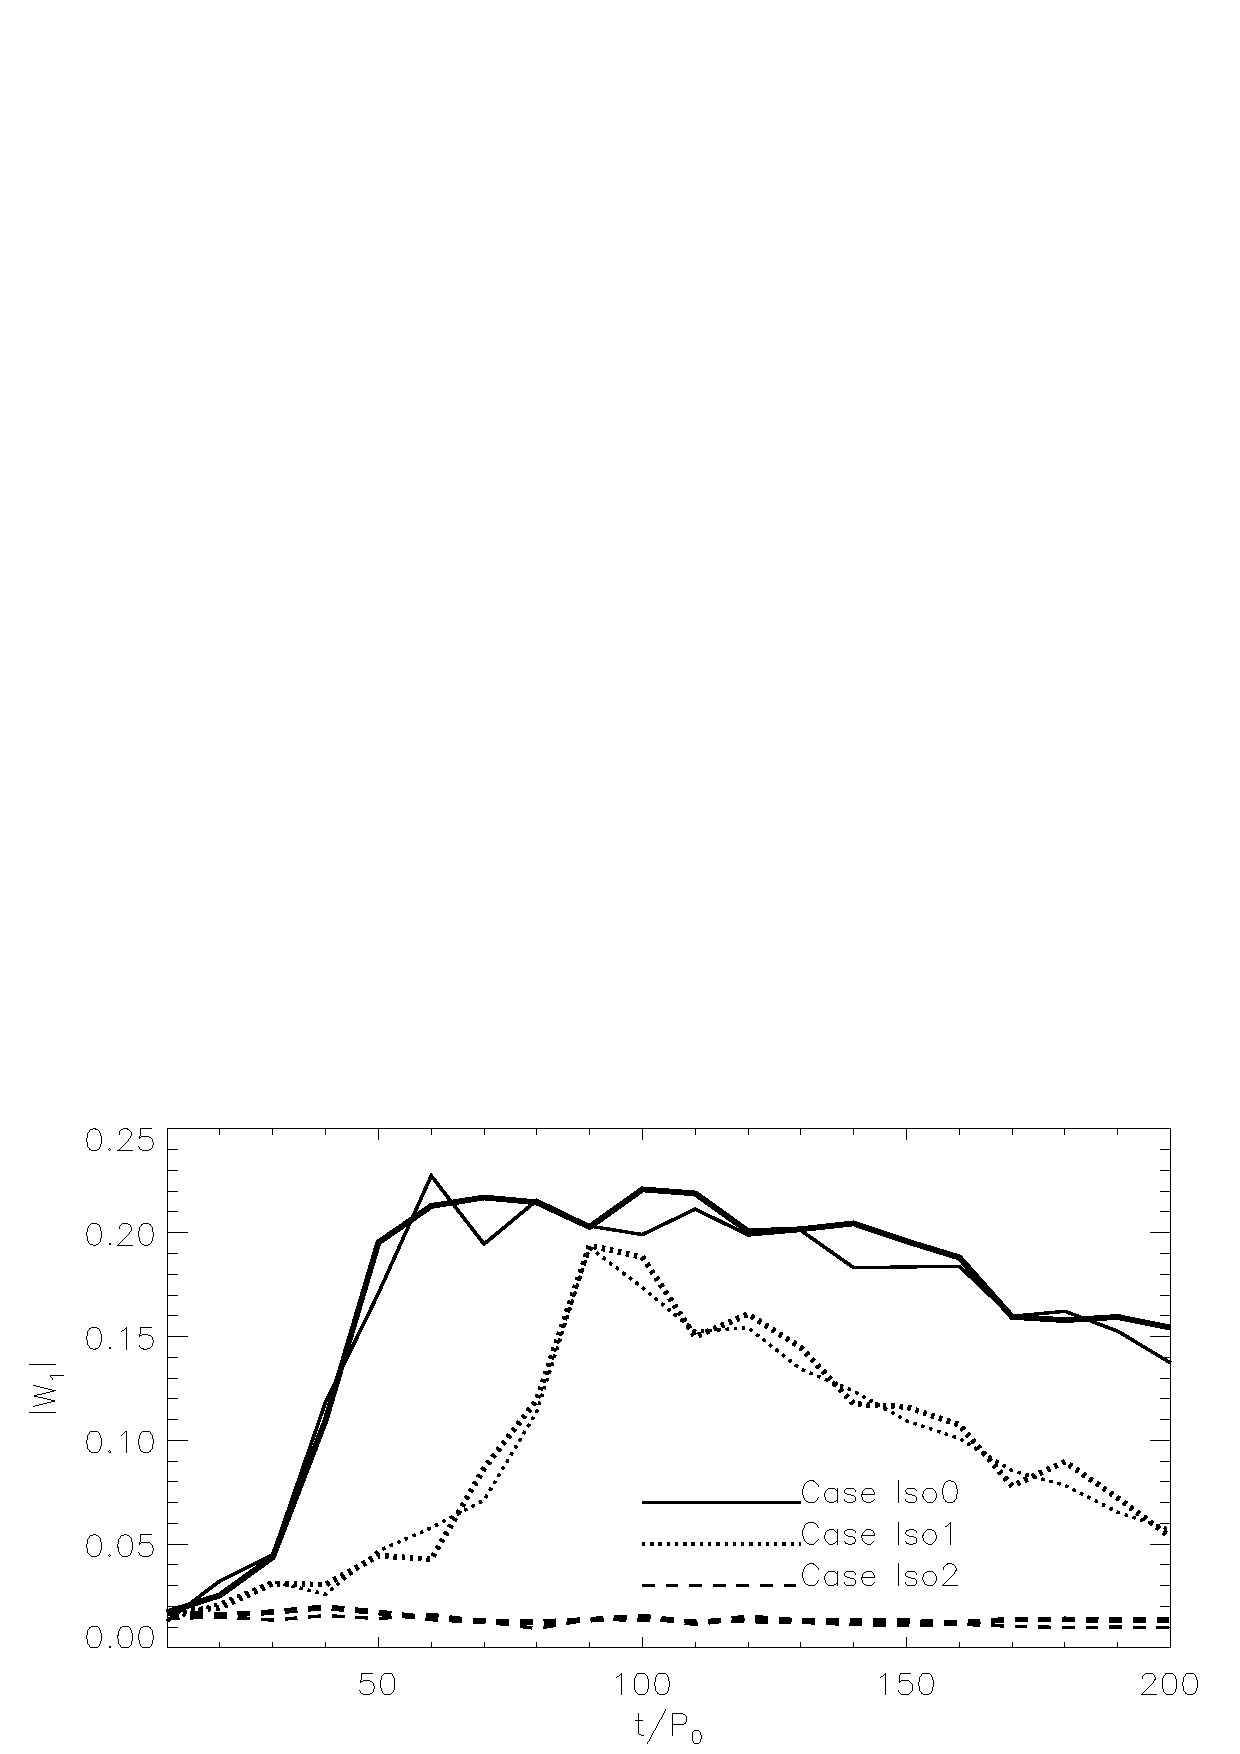
\includegraphics[width=\linewidth]{figures/pdisk_kerz_cases_iso}
  \caption{Same as Fig. \ref{pdisk_kerz_cases_planet} but for strictly
    isothermal Iso0 (solid, no viscous layer so $\hat{\nu}\sim10^{-6}$), Iso1
    (dotted, viscous layer with $\hat{\nu}\sim10^{-5}$) and Iso2
    (dashed, viscous layer with $\hat{\nu}\sim10^{-4}$). The thick (thin) lines indicate
    $W_1$ averaged over $\tan{\psi}\in[0,2]h$
    ($\tan{\psi}\in[2,3]h$).  
    \label{pdisk_kerz_cases_planet_iso}}
\end{figure}

%%\section{Discs with radial viscosity transitions}\label{dead}
Vortex-formation in at dead zone can boundaries in protoplanetary
discs ca be modeled by imposing a radially-structured viscosity
profile \citep{varniere06,crespe11} in  hydrodynamic simulations, or
more recently by directly simulating a magnetized disc with a
radially-structured resistivity \citep{lyra12}. These disc models are
either 2D or unstratified 3D,  implying the transition occurs at a
fixed cylindrical radius independent of height. Vortices observed in
such simulations have been attributed to the RWI, presumably because
of the PV extremum that results from mass build-up at the (effective)
viscosity jump. No corresponding linear stability
calculations have been performed to date, however, since the `basic
state' is time-dependent.       

In this section, we generalize the above studies by  
introducing viscous layers. We explore vortex formation at the
radial boundary between of high/low viscosity regions of the disc, 
when there exists a vertical viscosity transition as well.     

\subsection{Radially and vertically structured viscosity profile}
We adopt a similar viscosity profile as used for disc-planet
simulations, but modify it by a radial smooth-step function $f(R)$, 

\begin{align}\label{dead_profile}
  &\hat{\nu}\frac{\Sigma_i(R)}{\Sigma_i(r_0)}\frac{d\ln{\Omega_i}}{d\ln{R}} = 
  \hat{\nu}_0\left\{ \left[1+Q(\psi)\right]f + \left[ 1-
    f\right]A_\nu\right\}%\notag\\
  %  \phantom{\hat{\nu}\Sigma_i(R)\frac{d\ln{\Omega}}{d\ln{R}} =}
  \left.\frac{d\ln{\Omega_i}}{d\ln{R}}\right|_{r_0},\\
  &f(R) \equiv \frac{1}{2}\left[ 1 + \tanh{\left(\frac{R-r_0}{\Delta R_\nu}\right)} \right].
\end{align}
For $R>r_0$, the viscosity profile is the same as that used in the
previous section, while for $R<r_0$ the viscosity is uniform with 
$\hat{\nu}\sim A_\nu\hat{\nu}_0$. We set $\hat{\nu}_0=10^{-6}$ and
$A_\nu=10$. The radial transition width is fixed to $\Delta R_\nu =
0.5H_0$. As before the angular transition width is fixed to
$\zeta_\nu=0.2h$. An example of the viscosity profile produced by
Eq. \ref{dead_profile} is shown in Fig. \ref{visc2d_dead}.   

\begin{figure}
  \centering
  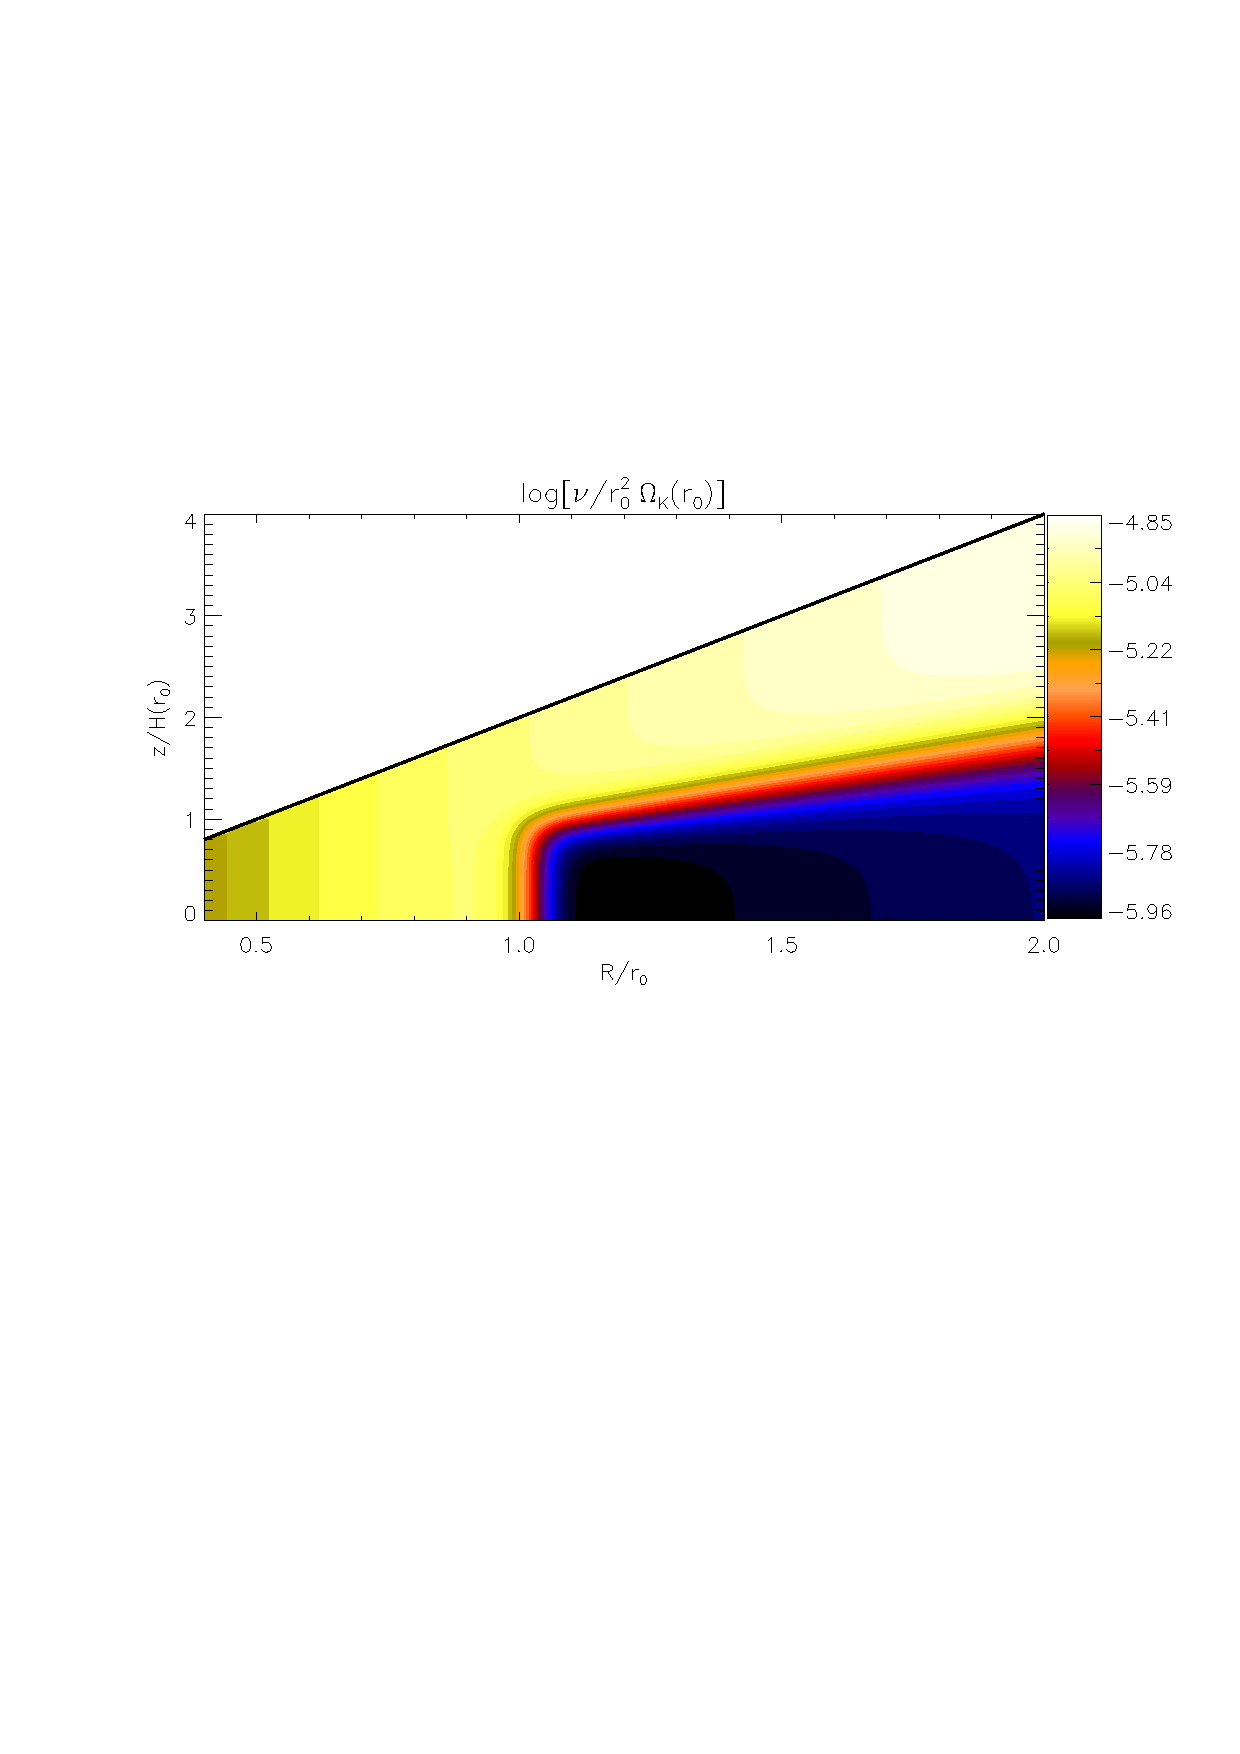
\includegraphics[width=\linewidth]{figures/pdisk_visc2d_dead}
  \caption{Example of the radially-and-vertically structured viscosity
    profile described by Eq. \ref{dead_profile}. 
    This specific plot case D2. The solid line delineates the upper
    boundary of the computational domain. 
    \label{visc2d_dead}}
\end{figure}

\subsection{Setup}
We consider discs with $h=0.1$, radial range
$[\rin,\rout]=[0.4,2.0]r_0$ and vertical size $n_h=2$. No surface
density bump is used ($A=1$). The resolution
is $(N_r,N_\theta,N_\phi)=(256,64,512)$. We initialize the disc
without radial flow, but impose perturbations to $v_r$ just after
initialization. Note that the initial condition is not a steady-state
equilibrium solution.   

\subsection{Dead zone simulations}
Our fiducial simulation, case D0, does not have a viscous layer in the
vertical direction. We then consider cases D1 
and D2 with angular transitions at $\zeta_\nu=1.5h$ and
$\zeta_\nu=1.0h$, which gives a viscous layer occupying
$25\%$ and $50\%$ of the uppermost vertical domain. That is, the 
viscous layer at unit radius has thickness $0.5H_0$ and $H_0$ for
cases D1 and D2, respectively. Table \ref{dead_sims} summarizes the
simulations in this section. 
 
\begin{table}
  \centering
  \caption{Summary of dead zone simulations. These runs employ the viscosity profile 
    described by Eq. \ref{dead_profile}, which involves a viscosity
    transition both radially and vertically. The viscous layer is quoted
    as a fraction of the vertical domain at $R=r_0$. \label{dead_sims}}
  \begin{tabular}{lcccc}
    \hline\hline
    Case & $\Delta R_\nu/H_0$ & $A_\nu$ &$\zeta_\nu/h$ & visc. layer \\ 
    D0 &  0.5    &    10      &    n/a      & 0     \\%&      -0.21 \\
    D1 &  0.5     &    10     &    1.5      & $25\%$ \\% &    -0.28 \\
    D2 &  0.5     &    10     &    1.0      & $50\%$ \\%&     -0.08 \\
    \hline
  \end{tabular}
\end{table}


\subsection{Results}
To obtain an overview of disc evolution, we compare the minimum Rossby 
numbers near $R=r_0$ between cases D0, D1 and D2 in
Fig. \ref{rtrans_nuamp10_minrossby}. {\bf to be updated}.  The Rossby
number decreases when non-axisymmetric disturbances develop at
the dead zone boundary. The non-smooth evolution signifies vortex
merging. Evidently, the evolutionary timescales vary between these
cases. So we compare them at similar evolutionary stages.   

%% Cases Db0 and Db1 evolve
%% similarly, with a time-shift between them. 
%% Over the course of the simulation, both cases reach a 
%% minimum Rossby number $\sim -0.3$ at $t\simeq 120P_0,\,170P_0$ for the
%% case Db0 and Db1, respectively. We find this minima coincided with
%% vortex merging, the result being a single vortex which subsequently elongates
%% and weakens. Case Db2 evolves quite differently, it attains a minimum Rossby
%% number of $Ro\simeq-0.08$ at $t=150P_0$. This is much weaker than the
%% two previous cases, but the vortex does not weaken afterwards ($|Ro|$
%% remains roughly constant for $t\gtrsim 150P_0$).  

\begin{figure}
  \centering
  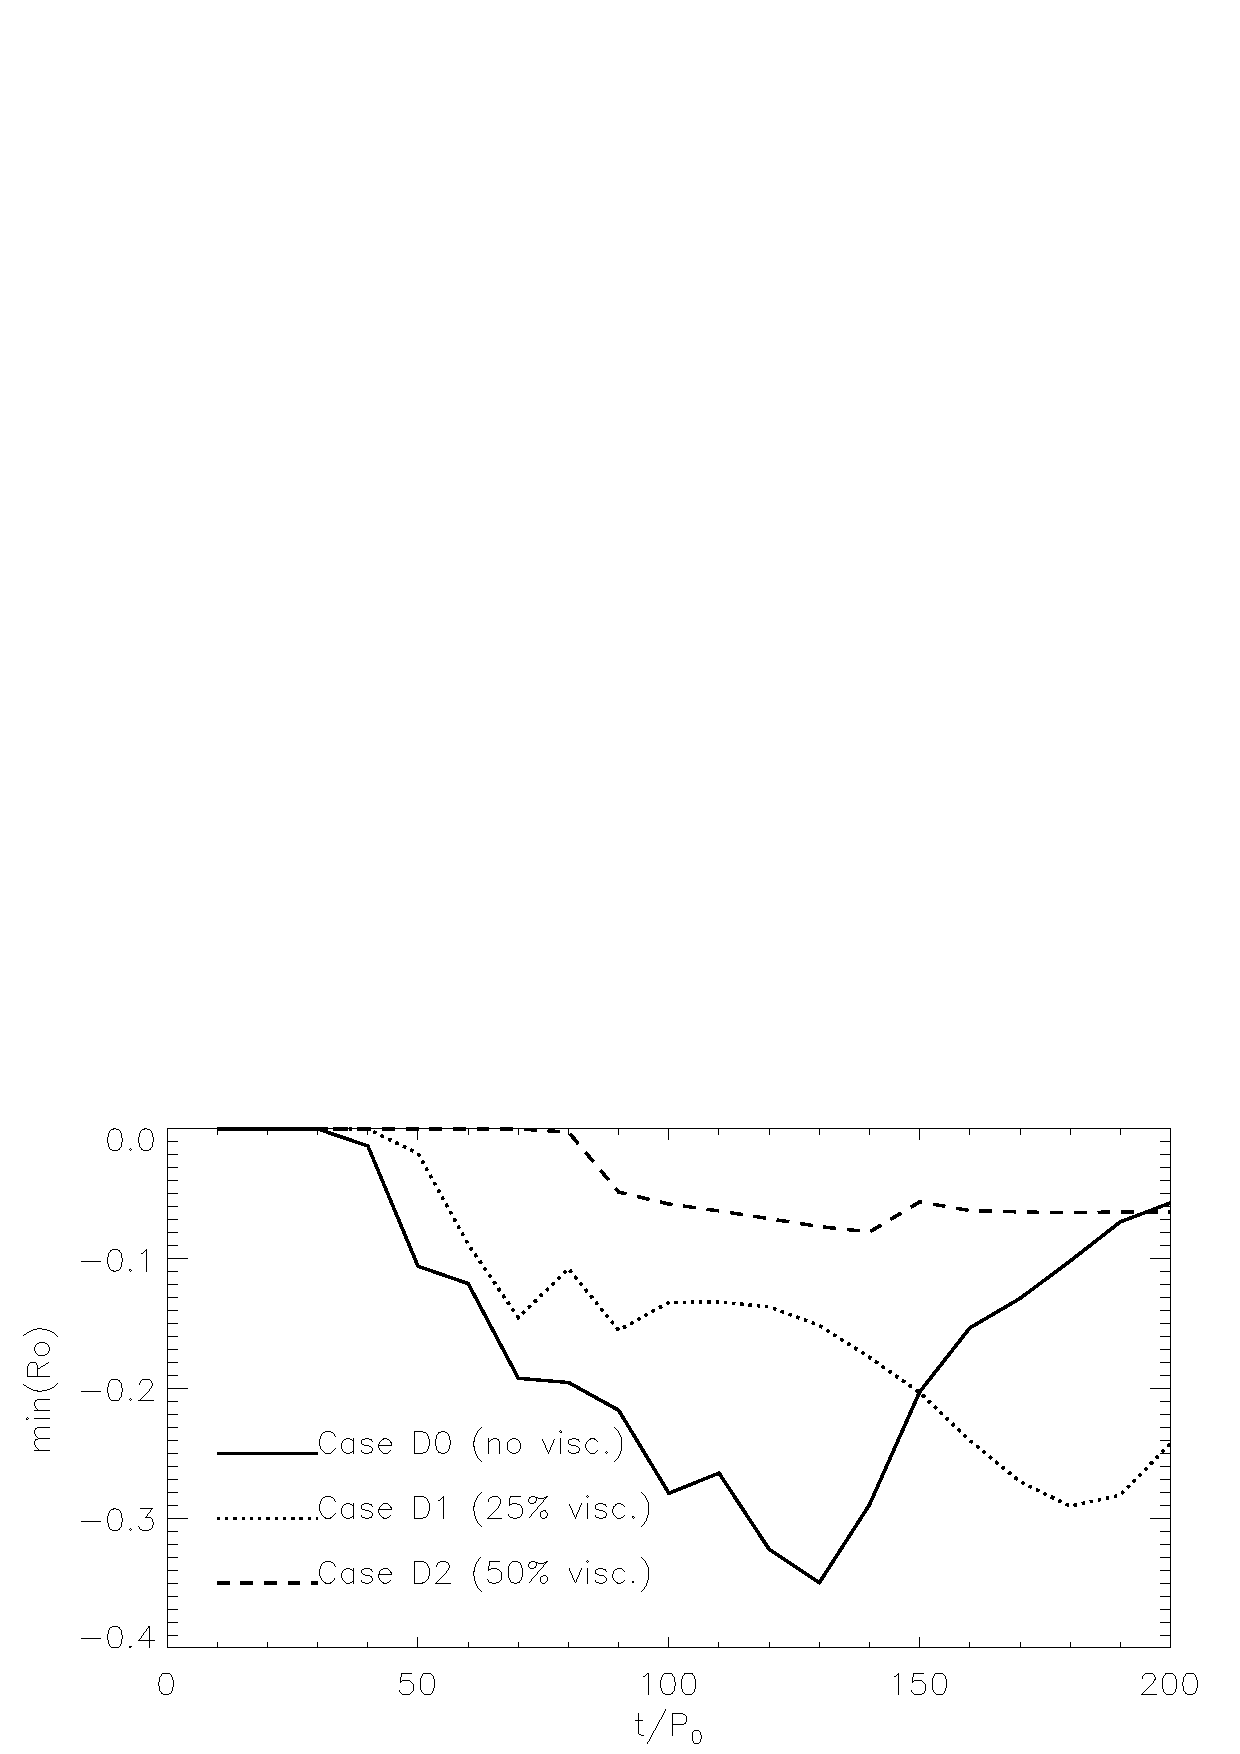
\includegraphics[width=\linewidth]{figures/rtrans_nuamp10_minrossby}
  \caption{Minimum midplane Rossby number found in case D0 (solid),
    D1, and D2 (dashed). The thickness of the viscous layer is quoted
    as the fraction of the uppermost vertical domain. 
    \label{rtrans_nuamp10_minrossby}}
\end{figure}

Fig. \ref{rtrans_nuamp10_vorten1d} shows the PV profiles as a result
of the mass build-up at the dead zone boundary. The snapshot for each
case is taken just before $Ro$ begins to decrease. 
The latter is necessary for the RWI. We
therefore consider these profiles as the `basic state' for the
RWI. Although convenient, this is not strictly correct because the
profiles in Fig. \ref{rtrans_nuamp10_vorten1d} do not correspond to
steady states, with respect to which a linear instability is defined.   

The radial viscosity transition leads to a PV maximum and a PV minimum
on either side of unit radius. The latter is associated with the RWI. 
Case D0 and D1 have very similar profiles, while the PV minimum is
slightly less sharp in case D2. Thus, the disc profile necessary for
instability is affected by the presence of a viscous layer. We expect
the RWI to grow more slowly in case D2 than the other cases. 

\begin{figure}
  \centering
  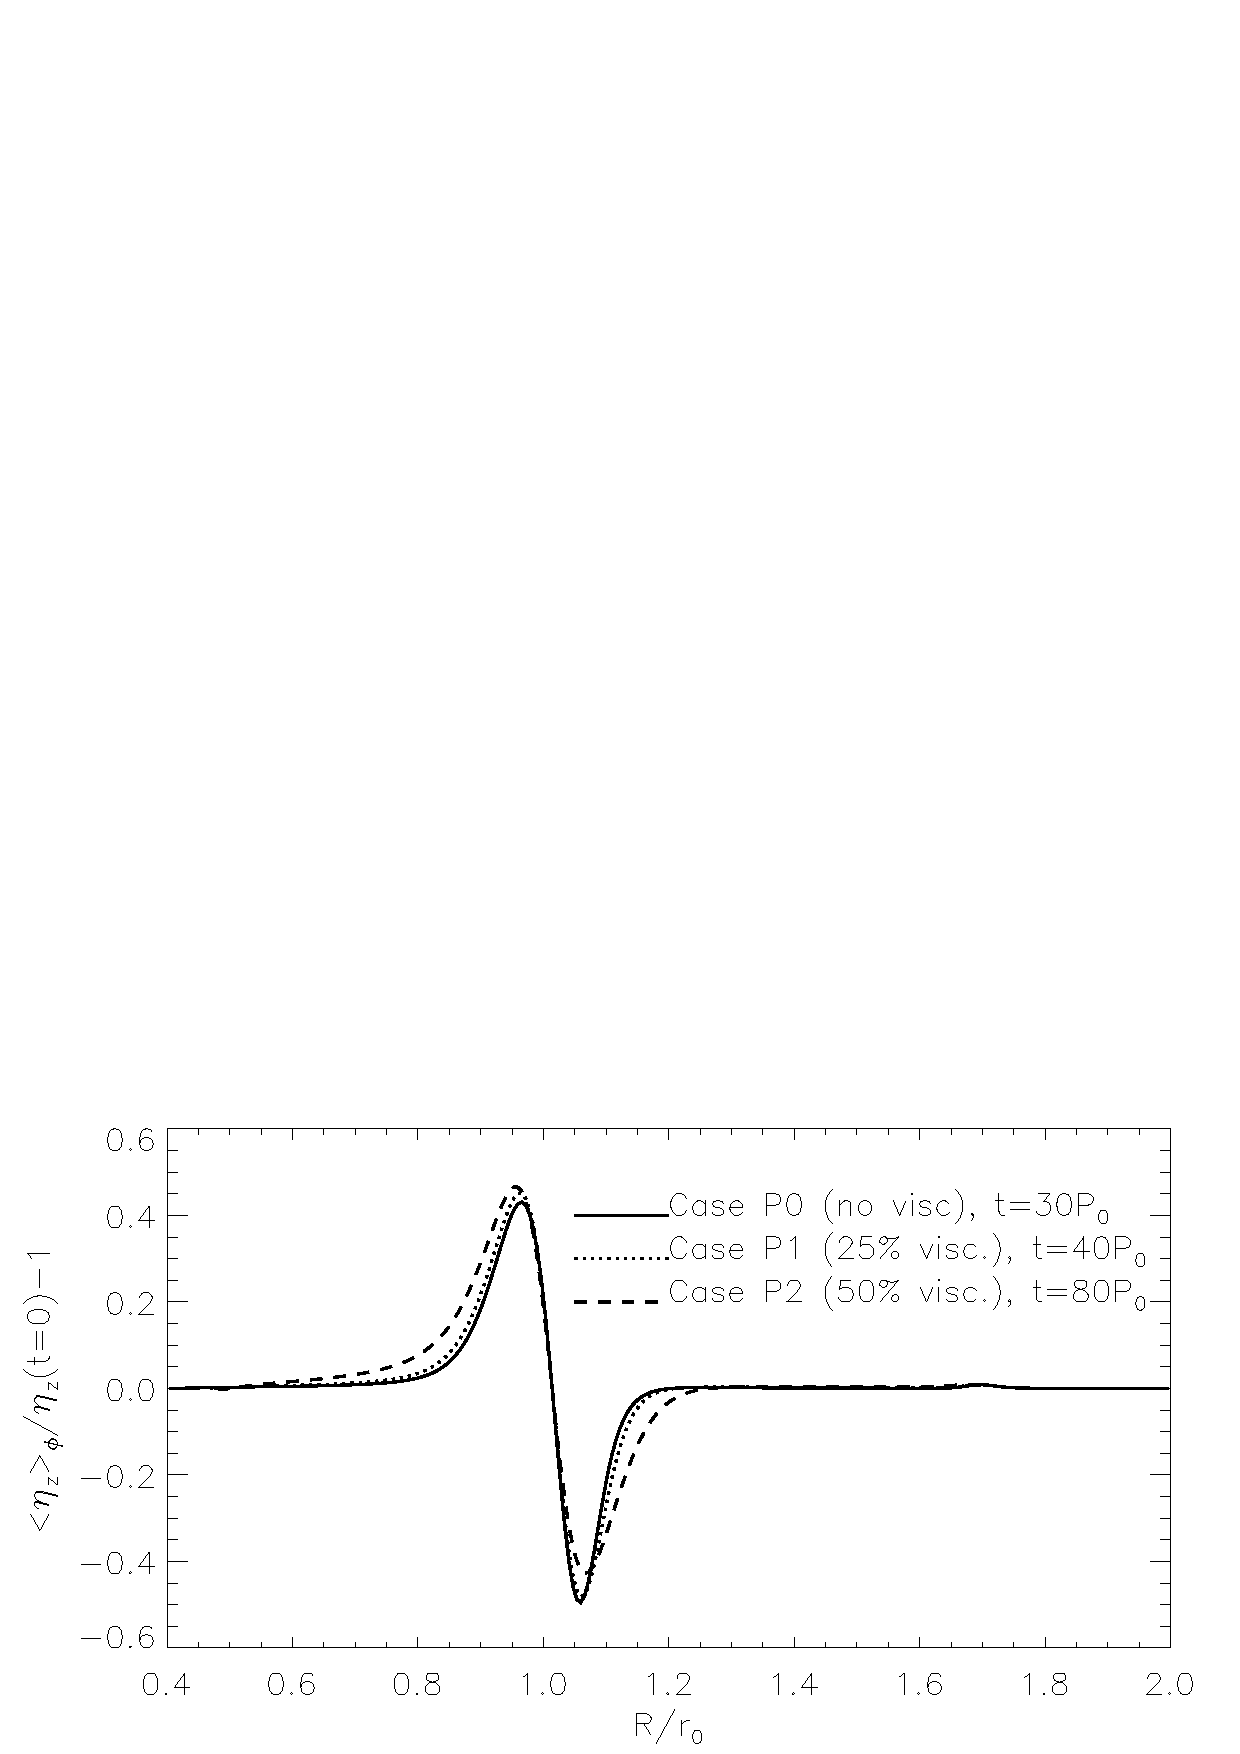
\includegraphics[width=\linewidth]{figures/rtrans_nuamp10_vorten1d}
  \caption{Potential vorticity profiles for dead zone simulations D0,
    D1 and D2. The snapshots are taken just before the Rossby numbers
    in Fig. \ref{rtrans_nuamp10_minrossby} first begins to decrease. 
    \label{rtrans_nuamp10_vorten1d}}
\end{figure}

Fig. \ref{rtrans_vdamp0_nuamp10} compares $\delta\rho$ at
$t=50P_0,\,60P_0$ and $100P_0$ for cases D0, D1 and D2, respectively.
The snapshots correspond to initial vortex formation. It is also when
the midplane $\min(Ro)$ first becomes non-negligible (see
Fig. \ref{rtrans_nuamp10_minrossby}). As expected from the PV
profiles, cases D0 and D1 are very similar, both developing the $m=3$
mode. However, case D2 develops the $m=2$ mode, because the PV extrema
is smoother. 

With the observed azimuthal wavenumbers in
Fig. \ref{rtrans_vdamp0_nuamp10}, we estimate the non-axisymmetric
mode growth rates to be $q_3\sim 0.1\Omega_0,\,0.09\Omega_0$ for cases D0 and D1; and
$q_2\sim0.05\Omega_0$ for case D2. The co-rotation radii were
%rates 0.11, 0.093 and 0.049
$r_c\sim1.073r_0,\,1.075r_0$ and $1.081r_0$, which are very close to
the radii of PV minima in Fig. \ref{rtrans_nuamp10_vorten1d}. Note
that the growth timescale is a few $P_0$, which is shorter than the
timescale to attain the PV extrema.  

\begin{figure}
   \centering
   \includegraphics[scale=.27,clip=true,trim=0cm 0.0cm 0cm
     0cm]{figures/rtrans_vdamp0_nuamp10_pdisk005.ps}\includegraphics[scale=.27,clip=true,trim=2.3cm
     0.0cm 0cm
     0cm]{figures/rtrans_vdamp2_nuamp10_pdisk006.ps}\includegraphics[scale=.27,clip=true,clip=true,trim=2.3cm
     0.0cm 0cm
     0cm]{figures/rtrans_vdamp3_nuamp10_pdisk010.ps}%% \\
    %% \includegraphics[scale=.27,clip=true,trim=0cm 1.84cm 0cm
    %%  .99cm]{figures/rtrans_vdamp0_nuamp10_vort005.ps}\includegraphics[scale=.27,clip=true,trim=2.3cm
    %%  1.84cm 0cm
    %%  0.99cm]{figures/rtrans_vdamp2_nuamp10_vort006.ps}\includegraphics[scale=.27,clip=true,clip=true,trim=2.3cm
    %%  1.84cm 0cm
    %%  0.99cm]{figures/rtrans_vdamp3_nuamp10_vort009.ps}
   \caption{Density perturbation $\delta\rho$ for dead zone simulations
     D0 (left), D1 (middle), and D2 (right). The snapshots are
     taken when $\max[\delta\rho(z=0)]$ first exceeds 0.2. 
     \label{rtrans_vdamp0_nuamp10}}
\end{figure}

%% In Fig. \ref{rtrans_vdamp0_nuamp10_2} we compare the final vortex just after its formation
%% (when $Ro$ reaches its minimum with respect to time). 
%% Cases Db0 and Db1 are again similar, developing a compact vortex with $Ro \sim -0.3$. However,
%% we found that this vortex weakens thereafter. On the other hand case Db2 , despite forming
%% a weaker vortex ($Ro\sim -0.07$).

The minimum midplane Rossby number attained is
$\min[Ro(z=0)]=-0.35,\,-0.29,\,-0.08$ for cases D0, D1 and D2,
respectively. The corresponding density perturbation is shown in
Fig. \ref{rtrans_vdamp0_nuamp10_2}. The vortex in case D1 is only slightly
weaker and larger than D0. However, snapshot for D1 is taken about
$50P_0$ later than D0. This, together with the above results,
indicates that introducing a relatively small viscous layer (recall
case D1 has a viscous layer of thickness $0.5H_0$) mainly shifts the
time evolution. In other words, the timescale required for vortex
formation is lengthened by introducing the viscous layer, but the
characteristics of the final vortex is not much affected. 

Case D2, on the other hand, evolves differently. It only attains
$\min[Ro(z=0)]= -0.08$ so the vortices are noticeably weaker than
cases D0/D1, as is the density fluctuation $\delta\rho$. As shown
in Fig. \ref{rtrans_vdamp0_nuamp10_2}, the vortex in case D2 is much
more elongated than previous runs. This is somewhat surprising because
the basic states are not significantly different (with similar growth
rates). 
%% Also in case D2 $Ro$ remains roughly
%% constant after reaching its minimal value, while in cases D0/D1
%% the vortex becomes weaker toward the end of the runs. 
%Also consistent with previous simulations, vortex-merging
%is resisted. 

\begin{figure}
   \centering
   \includegraphics[scale=.27,clip=true,trim=0cm 0.91cm 0cm
     0cm]{figures/rtrans_vdamp0_nuamp10_pdisk013.ps}\includegraphics[scale=.27,clip=true,trim=2.3cm
     .91cm 0cm
     0cm]{figures/rtrans_vdamp2_nuamp10_pdisk018.ps}\includegraphics[scale=.27,clip=true,clip=true,trim=2.3cm
     .91cm 0cm
     0cm]{figures/rtrans_vdamp3_nuamp10_pdisk014.ps}\\
    \includegraphics[scale=.27,clip=true,trim=0cm 0.cm 0cm
      .99cm]{figures/rtrans_vdamp0_nuamp10_vort013.ps}\includegraphics[scale=.27,clip=true,trim=2.3cm
      0.0cm 0cm
      0.99cm]{figures/rtrans_vdamp2_nuamp10_vort018.ps}\includegraphics[scale=.27,clip=true,clip=true,trim=2.3cm
      0.0cm 0cm
      0.99cm]{figures/rtrans_vdamp3_nuamp10_vort014.ps}
    \caption{Density perturbation $\delta\rho$ (top) and
      Rossby number $Ro$ (bottom) for cases D0 (left), D1
      (middle), and D2 (right). Snapshots are taken when
      $\mathrm{min}[Ro(z=0)]$ is attained. 
      \label{rtrans_vdamp0_nuamp10_2}}
\end{figure}


%\clearpage
\section{Summary and discussion}\label{summary}
We have performed customised hydrodynamic simulations of
non-axisymmetric instabilities in 3D viscous discs. We adopted
height-dependent kinematic viscosity profiles, such that the disc
midplane is of low viscosity ($\alpha\sim 10^{-4}$) and the disc
atmosphere is of high viscosity ($\alpha\sim 10^{-2}$). We were motivated  
by the question of whether or not the Rossby wave instability, and
subsequent vortex formation, operates in layered accretion discs.  

We first considered viscous disc equilibria with a radial density
bump and varied the vertical dependence of viscosity. 
This setup can isolate the effect of viscosity on the
linear RWI. We found that the linear RWI is unaffected by viscosity,
layered or not. The viscous RWI remains dynamical and lead to vortex
formation on timescales of a few 10s of orbits. We continued these
simulations into the non-linear regime, but found that vortices became
stronger as the viscous layer is increased in thickness. We suggest this
counter-intuitive result is an artifact of the chosen viscosity
profile because it is radially structured: viscosity attempts to
restore the equilibrium radial density bump, which favours the
RWI. This effect outweighs viscosity damping the linear instability. 

We also simulated vortex formation at planetary gap edges in layered
discs with a radially-smooth viscosity profile. %In this case viscosity
%only acts to damp the instability.  
Although vortex formation still 
occurs in layered discs, we found the vortex can be destroyed even when the viscous
layer only occupies the uppermost scale-height of the vertical domain
which is 3 scale-heights. This is significant because most of the disc
mass is contained within 2 scale-heights (i.e. the low viscosity
layer) but simulations show a viscous atmosphere inhibits long term
vortex survival.    
We found that the non-axisymmetric energy densities have
weak vertical dependence, so the disturbance evolves
two-dimensionally. It appears that applying a large viscosity in the
disc atmosphere is sufficient to damp the instability throughout the
vertical column of the fluid.

%We invoke the 3D vortex models described by \cite{barranco05} to
%explain why Rossby vortices are damped out even when viscosity is only
%applied in the disc atmosphere.  
\cite{barranco05} have described two 
3D vortex models: tall columnar vortices and short finite-height vortices. 
Rossby vortices are columnar, i.e. the associated vortex lines
extend vertically throughout the fluid column. One might have expected
an upper viscous layer to damp out vortex motion in the disc atmosphere, leading to a shorter
vortex. This, however, requires vortex lines to loop around the
vortex (the short vortex of \citeauthor{barranco05}). Such  
vortex loops form the surface of a torus \citep[see, for 
  example, Fig. 1 in][]{barranco05}, instead of ending on 
vertical boundaries. This implies significant vertical
motion near the vertical boundaries of the vortex, which would be  
difficult in our model because of viscous damping applied there. We
suspect this is why short/tall vortices fail to form/survive in our
layered disc-planet models.  Our results suggest that vortex
survival at planetary gap edges require low viscosity
($\alpha\lesssim10^{-4}$) throughout the vertical extent of the
disc.     


\subsection{Relation to other works}
%The work of \cite{pierens10} is most closely related to the present
%study.
\cite{pierens10} simulated the orbital migration of giant planets in
layered discs by prescribing a height-dependent viscosity profile. They
considered significant reduction in kinematic viscosity in going from
the disc atmosphere (the active zone, with $\alpha\sim10^{-2}$) to the
disc midplane (the dead zone, with $\alpha\sim10^{-7}$). According to
previous 2D simulations, such a low kinematic viscosity should lead to
the RWI \citep{valborro06,valborro07}. However, \citeauthor{pierens10}
did not report vortex formation, nor are vortices visible from their
plots. This result is consistent with our simulations. 

\cite{oishi09} carried out MHD shearing box simulations with 
a resistivity profile that varied with height to model a
layered disc: the disc atmosphere was MHD turbulent while the disc
midplane remained stable against the MRI. They envisioned the active
zone as a vorticity source for vortex formation in the midplane.  
Although their setup is fundamentally different to ours, they also
reported a lack of coherent vortices in the dead zone. They argued
that the MHD turbulence in the active layer was not sufficiently strong
to induce vortex formation in the dead zone. If MHD turbulence can be
represented by a viscosity, the lack of tall columnar vortices in
\citeauthor{oishi09} is consistent with our results. That is,
even when MRI turbulence is only present in the disc atmosphere it is
able to damp out columnar vortices.     

\subsection{Caveats and outlooks}\label{caveats}
%We stress that the goal of the present study is to demonstrate the
%potential impact of disc vertical structure on Rossby vortices. We
%adopted simple 

The most important caveat of the current model is the viscous
prescription to mimic MRI turbulence. In doing so, an implicit
averaging is assumed \citep{balbus99}. The spatial averaging should be
taken on length scales no less than the local disc scale-height, and
the temporal average taken on timescales no less than the local
orbital period. These are, however, the relevant scales for vortex
formation via the RWI. Furthermore, our viscosity profile varies on
length-scales comparable to or even less than $H$ (e.g. the vertical transition
between high and low viscosity layers). Nevertheless, as a proof of
concept, our simulations do demonstrate %that viscous damping can
%significantly 
the importance of disc vertical structure on the RWI. That is, damping,
even confined to the disc atmosphere, can destroy Rossby vortices. 

Another drawback of a hydrodynamic viscous disc model is the
fact that it cannot mimic magneto-elliptic instabilities (MEI), which
are known to destroy vortices in magnetic discs
\citep{lyra11,mizerski12}. A natural question is how 
Rossby vortices are affected by the MEI when it only operates in
the disc atmosphere. Extension of the present work to global non-ideal
MHD simulations will be necessary to address RWI vortex formation in
layered discs.   

However, some improvements can be made within the viscous
framework. A static viscosity profile neglects the
back-reaction of the density field on the kinematic viscosity. Thus,
our simulations only consider how Rossby vortices 
respond to an externally applied, axisymmetric viscous damping. A more
physical viscosity prescription should depend on the local column density
\citep{fleming03}, with viscosity decreasing with increasing column
density. The effective viscosity inside Rossby vortices would be
lowered relative to the background disk because disc vortices are
over-densities. If the over-density is large, then it is
conceivable that the vortex formation itself may render the effective
viscosity to be sufficiently low throughout the fluid column to allow
long term vortex survival.    
Preparation for this study is underway and results will be reported in
a follow-up paper. 


\section*{Acknowledgments}
This work benefited from extensive discussion with O. Umurhan. I also
thank R. Nelson for discussion{\bf, and M. de Val-Borro} for a
helpful report.   Computations were performed on the
CITA Sunnyvale cluster, as well as the GPC supercomputer at the SciNet
HPC Consortium. SciNet is funded by the Canada Foundation for
Innovation under the auspices of Compute Canada, the Government of
Ontario, Ontario Research Fund – Research Excellence and the
University of Toronto.   

\bibliographystyle{mn2e}
\bibliography{ref}

\appendix
{\bf
%  \subsubsection{Simulations without a radial}
  \section{Artificial radial density bumps with a radially smooth
    viscosity profile}\label{add_sim}
  In \S\ref{density_bump} we found that vortices became stronger
  as the viscous layer thickness is increased, even though linear growth rates
  were reduced. Here, we present additional simulations to support the 
  hypothesis that this is due to the localised radial structure in the viscosity profile. 

  We repeated simulation V2 (see Table \ref{artificial_bump})
  with a radially-smooth viscosity profile given by 
  \begin{align}\label{smooth_visc}          
    \hat{\nu}\frac{\rho_i(R,z)}{B(R)} =
    \hat{\nu}_0\left[1+Q(z/H_0) \right]\frac{\rho_i(r_0,z)}{B(r_0)}. 
  \end{align}                  
  We set the floor viscosity $\hat{\nu}_0=10^{-7}$ to mitigate
  axisymmetric viscous diffusion of the initial density bump. The
  viscous layer with $\hat{\nu} \sim 10^{-5}$ occupies $z\in[1,2]H_0$
  at $R=r_0$.   
                      
  This simulation is shown as the dotted line in Fig. \ref{appen} in
  terms of the $m=1$ component of the kinetic energy density. We
  compare it to the corresponding case using the radially-structured
  viscosity profile in \S\ref{density_bump}. Vortex formation occurs
  in both runs.  
  With a radially-smooth viscosity profile, the vortex decays 
  monotonically after $|W_1|$ reaches maximum value of $\sim 0.05$. 
  Using the radially-structured viscosity profile (solid line) gives a
  larger disturbance amplitude at the linear stage  ($\max{|W_1|}\sim
  0.08$), and although it subsequently decays, the decay is halted for
  $t\gtrsim110P_0$.    

  The contrast between these cases show that the radial structure
  in the viscosity profile helps vortex survival. This experiment
  indicates that the dominant effect of viscosity is its
  influence on the evolution of the axisymmetric part of background
  disc. The radially-structured viscosity profile is a source for the
  radial PV minimum, which is needed for the RWI.  

  Our result here is qualitatively similar that in \cite{regaly12},
  where a sharp viscosity profile was imposed in a 2D simulation and 
  vortex formation ensues via the RWI. The vortex eventually
  disappears, but re-develops after the system returns to a
  axisymmetric state. This is because the imposed viscosity profile
  causes the disc to develop the required PV minimum for the RWI. 

 \begin{figure}
  \centering
  %  \includegraphics[scale=.41,clip=true,trim=0cm 1.cm 0cm 0cm]{figures/pdisk_kerz_cases_appendix.ps}
  \includegraphics[width=\linewidth]{figures/pdisk_kerz_cases_appendix1.ps}
  \caption{ {\bf Evolution of the $m=1$ component of the kinetic energy
    density, averaged over the shell $r\in[0.8,1.2]r_0$, for a layered 
    disc initialised with a radial density bump. 
    The solid line employs the viscosity profile given by 
    Eq. \ref{visc_profile}, while the dotted line employ the radially-smooth
    viscosity profile given by Eq. \ref{smooth_visc}.}\label{appen}}
  \end{figure}

}

%\input{appendix2}

\end{document}
